% !TeX encoding = UTF-8
% !TeX spellcheck = en_US
% !BIB program=biber
\PassOptionsToPackage{dvipsnames}{xcolor}
\documentclass[journal]{IEEEtran}




\usepackage{etoolbox}

\usepackage{xr}
\externaldocument{supplementary}

\usepackage[%
style=numeric-comp,%
sortcites=true,%
sorting=none,%
url=false,%
doi=false,%
eprint=false,%
isbn=false,%
]{biblatex}
\addbibresource{abrv.bib}
\addbibresource{paper.bib}


\usepackage{graphicx}
\graphicspath{{./img/}}
\usepackage[labelformat=simple]{subcaption}
\captionsetup{font=footnotesize, labelfont={bf}, labelsep=period}
\renewcommand\thesubfigure{(\alph{subfigure})}
\renewcommand\thesubtable{(\alph{subtable})}

\newcommand{\boximg}[2]{\parbox[c]{#1\subfigsz}{\includegraphics[width=#1\subfigsz]{#2}}}

\usepackage{tikz}
\usepackage{pgfplots}
\usepackage{pgfplotstable}
\pgfplotsset{compat=1.16,
  grid style=dashed,
  ymajorgrids=true,
}

\newlength{\subfigsz}

\usetikzlibrary{
  calc,
  shapes,
  arrows,
  shadows,
  positioning,
  decorations.shapes,
  decorations.markings,
  fit,
  bayesnet,
  matrix,
}

\usepgfplotslibrary{
  groupplots,
  colorbrewer,
  statistics,
  fillbetween,
}


\usepackage{booktabs}           %
\usepackage{multirow}
\usepackage{arydshln}           %


\usepackage{siunitx}
\sisetup{
  separate-uncertainty,
  table-format=1.2(3),
  detect-all,
}
\robustify\bf

\makeatletter
\def\adl@drawiv#1#2#3{%
  \hskip.5\tabcolsep
  \xleaders#3{#2.5\@tempdimb #1{1}#2.5\@tempdimb}%
  #2\z@ plus1fil minus1fil\relax
  \hskip.5\tabcolsep}
\newcommand{\cdashlinelr}[1]{%
  \noalign{\vskip\aboverulesep
    \global\let\@dashdrawstore\adl@draw
    \global\let\adl@draw\adl@drawiv}
  \cdashline{#1}
  \noalign{\global\let\adl@draw\@dashdrawstore
    \vskip\belowrulesep}}
\makeatother

\usepackage{pdflscape}


\usepackage{amsmath}
\interdisplaylinepenalty=2500
\usepackage{mathtools}
\usepackage{commath}
\usepackage{amsfonts}           %
\usepackage{nicefrac}           %
\usepackage{microtype}          %

\newcommand{\conc}{\mathbin{\Vert}}


\DeclarePairedDelimiterX{\infdivx}[2]{(}{)}{%
  #1\;\delimsize\|\;#2%
}
\newcommand{\kl}{\operatorname{KL}\infdivx}
\newcommand{\skl}{\operatorname{SKL}\infdivx}

\newcommand{\rpm}{\raisebox{.2ex}{$\scriptstyle\pm$}}

\newcommand\givenbase[1][]{\:#1\lvert\:}
\let\given\givenbase

\newcommand\reallywidehat[1]{\ThisStyle{%
  \setbox0=\hbox{$\SavedStyle#1$}%
  \stackengine{-1.0\ht0+.5pt}{$\SavedStyle#1$}{%
    \stretchto{\scaleto{\SavedStyle\mkern.15mu\char'136}{1.5\wd0}}{1.4\ht0}%
  }{O}{c}{F}{T}{S}%
}}
\newcommand{\hkl}{\widehat{\operatorname{KL}}\infdivx}

\newcommand{\CI}{\mathrel{\perp\mspace{-10mu}\perp}}

\DeclareMathOperator*{\argmax}{arg\,max}
\DeclareMathOperator*{\argmin}{arg\,min}

\makeatletter
\DeclareRobustCommand\bigop[1]{%
  \mathop{\vphantom{\sum}\mathpalette\bigop@{#1}}\slimits@
}
\newcommand{\bigop@}[2]{%
  \vcenter{%
    \sbox\z@{$#1\sum$}%
    \hbox{\resizebox{\ifx#1\displaystyle.9\fi\dimexpr\ht\z@+\dp\z@}{!}{$\m@th#2$}}%
  }%
}
\makeatother

\DeclareMathOperator*{\E}{\mathbb{E}}

\let\oldtimes\times
\def\times{{\mkern1mu\oldtimes\mkern1mu}}

\makeatletter
\DeclareRobustCommand{\rvdots}{%
  \vbox{
    \baselineskip4\p@\lineskiplimit\z@
    \kern-\p@
    \hbox{.}\hbox{.}\hbox{.}
}}
\makeatother


\usepackage{algorithm}
\usepackage{algorithmic}

\PassOptionsToPackage{hyphens}{url}
\usepackage{hyperref}
\hypersetup{
  colorlinks,
  linkcolor = BrickRed,
  citecolor = NavyBlue,
  urlcolor  = WildStrawberry,
}
\usepackage{url}


\usepackage{xspace}
\makeatletter
\DeclareRobustCommand\onedot{\futurelet\@let@token\@onedot}
\def\@onedot{\ifx\@let@token.\else.\null\fi\xspace}

\def\eg{{e.g}\onedot} \def\Eg{{E.g}\onedot}
\def\ie{{i.e}\onedot} \def\Ie{{I.e}\onedot}
\def\cf{{cf}\onedot} \def\Cf{{Cf}\onedot}
\def\etc{{etc}\onedot} \def\vs{{vs}\onedot}
\def\wrt{w.r.t\onedot} \def\dof{d.o.f\onedot}
\def\etal{{et al}\onedot}  \def\aka{a.k.a\onedot}
\def\adhoc{{ad hoc}\xspace}
\makeatother


\hyphenation{op-tical net-works semi-conduc-tor}


\begin{document}

\title{Video Reenactment as Inductive Bias for Content-Motion Disentanglement}

\author{J.~F. Hernández~Albarracín,
        and A. Ramírez~Rivera,~\IEEEmembership{Senior Member,~IEEE}%
\thanks{%
Juan F. Hernández Albarracín is with Institute of Computing, University of Campinas, SP, Brazil, e-mail \texttt{juan.albarracin@ic.unicamp.br}.  Adín Ramírez Rivera is with Department of Informatics, University of Oslo, Norway, e-mail \texttt{adinr@uio.no}; and part of this work was done at the Institute of Computing, University of Campinas.}%
\thanks{Juan F. Hernández Albarracín was funded by the São Paulo Research Foundation (FAPESP) under grant No.~2017/16144-2.  A. Ramírez Rivera was funded by the Brazilian National Council for Scientific and Technological Development (CNPq) under grant No.~307425/2017-7; and in part by FAPESP under grant No.~2019/07257-3. Juan F. Hernández Albarracín and A. Ramírez Rivera were funded by the Coordena\c{c}\~ao de Aperfei\c{c}oamento de Pessoal de N\'ivel Superior---Brasil (CAPES)---Finance Code 001.}%
\thanks{The source code is available at \url{https://gitlab.com/mipl/mtc-vae}.}
%\thanks{This paper has supplementary downloadable material available at \url{http://ieeexplore.ieee.org}, provided by the author.  The material includes a supplementary document with additional results. Contact \texttt{adinr@uio.no} for further questions about this work.}
\thanks{Pre-print to appear in IEEE Trans.\ on Image Processing.}
\thanks{Digital Object Identifier \href{https://doi.org/10.1109/TIP.2022.3153140}{10.1109/TIP.2022.3153140}.}
}

\markboth{IEEE Transactions on Image Processing}%
{Hern\'andez~Albarrac\'{i}n \& Ram\'{i}rez~Rivera: Video Reenactment as Inductive Bias for Content-Motion Disentanglement}


\maketitle

\begin{abstract}
Independent components within low-dimensional representations are essential inputs in several downstream tasks, and provide explanations over the observed data.
Video-based disentangled factors of variation provide low-dimensional representations that can be identified and used to feed task-specific models.
We introduce MTC-VAE, a self-supervised motion-transfer VAE model to disentangle motion and content from videos.
Unlike previous work on video content-motion disentanglement, we adopt a chunk-wise modeling approach and take advantage of the motion information contained in spatiotemporal neighborhoods.
Our model yields independent per-chunk representations that preserve temporal consistency.
Hence, we reconstruct whole videos in a single forward-pass.
We extend the ELBO's log-likelihood term and include a Blind Reenactment Loss as an inductive bias to leverage motion disentanglement, under the assumption that swapping motion features yields reenactment between two videos.
We evaluate our model with recently-proposed disentanglement metrics and show that it outperforms a variety of methods for video motion-content disentanglement.
Experiments on video reenactment show the effectiveness of our disentanglement in the input space where our model outperforms the baselines in reconstruction quality and motion alignment.
\end{abstract}

\begin{IEEEkeywords}
Disentangled representations, Video reenactment, Variational inference, Generative models, Self-supervised learning.
\end{IEEEkeywords}

\IEEEpeerreviewmaketitle

\section{Introduction}
\label{sec:introduction}

\IEEEPARstart{W}{hile} the goal of representation learning is to obtain low-dimensional vectors useful for a diverse set of tasks, Disentangled Representation Learning (DRL) captures independent factors of variation within the observed data.
These disentangled representations are robust and interpretable, simplify several downstream tasks like classification and Visual Question Answering~\cite{Locatello2020aaai}, and support diverse content generation tasks~\cite{Chen2020tip,Ramesh2021}.
DRL shifted from unsupervised to weakly- and self-supervised methods, as inductive biases have shown to be fundamental in Deep Generative Models (DGM)~\cite{Locatello2019, Shu2020}.
DRL methods from video separate \emph{time independent} (\aka content) from \emph{dependent} (\aka motion) factors of variation.
While content features must be forced to have a low variance throughout the sequence, motion ones are expected to change.

Disentangling information from videos is of major importance since it can ease tasks that depend on the spatiotemporal data.
For instance, prediction tasks could rely on the independent representations of the objects or only on their temporal information.
These independence could not only ease the load on the downstream tasks but also enforce fairness and privacy over the data.
DRL from videos has been approached as a sequential learning process forcing temporal consistency among frames.
This problem is commonly addressed with Recurrent Neural Networks (RNN), due to their capacity of modeling temporal data of variable length.
Although architectures based exclusively on 3D Convolutional Neural Networks (3D-CNN) have been used in general representation learning from videos for downstream tasks~\cite{Carreira2017, Feichtenhofer2019}, few works rely only on convolutional architectures for DRL and posterior video generation~\cite{Wang2020, Aich2020}, despite their capacity of modeling whole videos, as they are constrained to fixed-length sequences.

Taking into account the great suitability of Variational Autoencoders (VAE) for unsupervised tasks~\cite{Su2020,Shi2018},
we propose a self-supervised DRL model that takes advantage of local spatio-temporal regularity to reconstruct videos by disentangling their content and motion while learning a robust representation space.
Motion-Transfer Chunk Variational Autoencoder (MTC-VAE) is a Variational Autoencoder that models temporal segments (\aka chunks) as independent random variables, maps them into a disentangled latent distribution, and maps them back consistently.
When modeling chunks as independent, the reconstructed videos may not be temporally consistent.
Hence, we preserve the temporal dependency that naturally exists among the chunks by assuming a Markovian relation between consecutive chunks at inference time.
To enforce it, we incorporate two inductive biases in our model:
(i)~We assume content features as stationary and motion ones as non-stationary in our model's log-likelihood.
(ii)~Video Reenactment (VR) is equivalent to swapping the motion representation of two videos and mapping them to the input space.
We show that this duality (independence at generation time, and dependence at inference time) is successful at representing video sequences for both disentanglement and reconstruction.

Our contributions are: (i)~A self-supervised DGM for VR and content-motion disentanglement from arbitrary-length videos through a simple 3D-CNN architecture in a single forward pass, improving over existing methods.
(ii)~Even assuming chunk independence, we significantly ease the disentangled motion-content feature inference and consistent video reconstruction, due to our inductive biases, and the self-supervised representation learning scheme.
(iii)~We show, that chunk-wise is better suited for DRL and video synthesis than frame-wise modeling for long videos.
Moreover, we highlight that, unlike SotA VR models, MTC-VAE is suited to learn disentangled low-dimensional representations.
VR models rely on entangled high-dimensional features and bypass information through the architecture to achieve better reconstruction at the cost of bloated features.
In contrast, our objective is to obtain independent factors of variation that are expressive enough for simple generators to create natural videos.

\section{Related Work}
\label{sec:soa}

\subsection{General Disentangled Representation Learning}
Seminal works on DRL are mostly unsupervised, and the majority rely on VAEs.
InfoGAN~\cite{Chen2016}, however, is the most relevant exception.
It uses control variables (categorical, discrete, or continuous) in the latent representation as inductive biases while penalizing mutual information among the latent units in an adversarial framework.
$\beta$-VAE~\cite{Higgins2017} includes the $\beta$ hyper-parameter into the VAE's ELBO to leverage independence among the latent scalars, leading to a higher-quality disentanglement.
Later approaches (\eg, $\beta$-TCVAE~\cite{Chen2018dr} and FactorVAE~\cite{Kim2018}) penalize Total Correlation among the latent scalars, yielding a better trade-off between disentanglement and reconstruction quality.
The ground-breaking work by \textcite{Locatello2019} showed that unsupervised methods for DRL are extremely weak.
Posterior works have shifted to weakly- and self-supervised approaches.
Hence, our proposed MTC-VAE introduces inductive biases in the latent space, such as explicit latent factors to represent content and motion features, with sufficient encoded information to guarantee VR from them.

\subsection{Disentangled Representations from Video}
\label{sec:soa_vdrl}
These works focus on disentangling time-dependent from time-independent features for each frame of the video and then enforcing inter-frame consistency.
Common setups of these approaches perform pose-content disentanglement while achieving consistency using RNNs and GANs~\cite{Denton2017, Villegas2017, Hsieh2018, Ge2018}.
Instead of pose-content disentanglement, some works separate deterministic from stochastic features~\cite{Denton2018, Lee2019savp}.
Most of the works in this area are applied to video prediction, but recent ones have started to be tested on VR tasks~\cite{Li2018,Wang2020,Aich2020,Zhu2020}.
Few of them \cite{Wang2020, Aich2020} rely on 3D-convolutional generators, but are constrained to fixed-length videos.
The rest use RNNs to capture the temporal relation between frames or segments at generation time, to perform either video reconstruction, prediction, or sequence-to-sequence translation.
Although MTC-VAE models dependent chunks at inference time, it assumes independence at generation time.
These assumptions simplify the tasks of reconstruction and VR since, to reconstruct a chunk of a video, it does not need to reconstruct the previous ones.
Therefore, the chunkwise approach takes the best of both worlds at not being constrained either to fixed-length-sequences or sequential generation.

\subsection{Video Reenactment}
\label{sec:soa_vr}
Recent methods on VR work in the domain of human faces~\cite{Zakharov2019, Nirkin2019, Chen2018, Zhou2019aaai}, human poses~\cite{Chan2019, Zhou2019, Liu2019tg, Yang2020}, or objects in general~\cite{Bansal2018, Siarohin2019, Siarohin2021, Zhao2018, Xie2020}.
Their main objective is to generate realistic videos, while the representation is either irrelevant or a secondary objective.
Instead, DRL models hold this objective as primary.
Most of these methods rely on warping techniques assisted by spatial transformer networks~\cite{Jaderberg2015} for frame-wise conditional video generation.
To apply such transformations, the generator requires high-dimensional spatial information that would normally be lost in a low-dimensional latent representation.
Hence, they either map to latent spaces that are larger than the original input space, to preserve spatial information, or bypass this information through skip connections from the encoder to the decoder.
Thus, a low-dimensional latent representation is not enough to represent the whole video.
In contrast, our proposal reconstructs videos while learning low-dimensional and factorized representations.
We highlight that our method reconstructs videos exclusively from low-dimensional representations.
Due to this restriction, we expect the perceptual quality and motion complexity of rendered videos to be higher in VR methods in comparison to DRL ones.
Despite this limitation, we consider our work as a step towards bridging these two areas.

\section{Proposed Approach: MTC-VAE}
\label{sec:method}

Given that content changes at a much slower rate than motion in a video, we propose to extract disentangled representations from local spatiotemporal neighborhoods (\aka chunks).
Content information of neighboring chunks changes so slowly that we may assume that it remains constant throughout a scene, while motion presents rapid changes.
Unlike existing frame-wise approaches, we use chunks to better capture the temporal characteristics of the video (\cf Section~\ref{sec:ablation} for the impact of the temporal windows), and their relations to obtain a self-supervised learning signal.

MTC-VAE contains only 3D-convolutional streams and, unlike recurrent approaches, models chunks as independent random variables for the generative pass, yet Markovian-dependent for the inference one.
Our formulation starts diverging from a standard two-latent-priors VAE when we extend our $\log p(x)$ to leverage inter-chunk consistency, which helps to reconstruct realistic videos, even though chunks are independently generated.
We go further and introduce the self-supervised \textit{blind reenactment loss} (BRL): another inductive bias that blindly simulates VR between two videos.

\subsection{Chunk-wise Video Modeling}
\label{sec:modeling}

We represent the video $x = (x_{k})_{k=1}^K$ as a sequence of $K$ non-overlapping and equally-sized chunks~$x_{k}$ of length $c$.%
\footnote{%
  For brevity, we assume that $c$ divides the length of the video.
  However, we can model arbitrary-length videos by padding incomplete chunks to match $c$.}
Similarly, we define $w = \left(w_k\right)_{k=1}^K$ as the sequence of motion representations of each~$x_k$.
For the $k$-th chunk, we model the content and motion as independent latent variables $z$ and $w_k$, respectively.
We assume $z$ to be unique and shared across the chunks, as content remains constant through time.
Fig.~\ref{fig:graphical_model} depicts the graphical model for a video~$x$.
\begin{figure}%
  \centering%
  \resizebox{0.5\linewidth}{!}{% !TeX root=../paper.tex
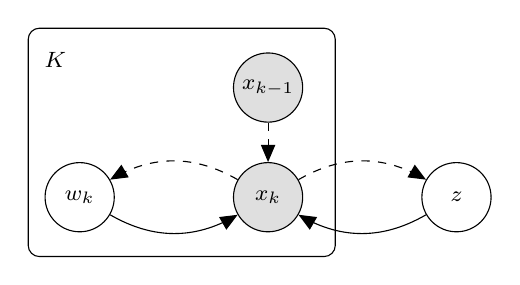
\begin{tikzpicture}[
  latent/.append style={
    minimum width=25pt,
    font=\footnotesize
  },
  plate caption/.append style={below right=0pt and 0pt of #1.north west},
]
\node[obs] (xk) {$x_k$};
\node[obs, above=.5cm of xk] (xkp) {$x_{k-1}$};
\node[latent, right=1.5cm of xk] (z) {$z$};
\node[latent, left=1.5cm of xk] (wk) {$w_k$};

\plate [inner sep=.3cm, xshift=0.1cm] {xw} {(wk)(xk)(xkp)} {$K$};
%\plate [inner sep=.5cm] {xwz} {(wk)(xk)(z)(xkp)} {$N$};

\path (wk) edge[bend right, ->] (xk);
\path (z) edge[bend left, ->] (xk);

\path (xk) edge[dashed, bend right, ->]  (wk);
\path (xk) edge[dashed, bend left, ->]  (z);
\path (xkp) edge[dashed, ->]  (xk);

\end{tikzpicture}

}
  \caption{%
  In the generative model (solid arrows), $K$ chunks $\{x_{k}\}$ (observed) share the same content~$z$, while having their own motion~$w_k$.
During inference (dashed arrows), the latent variables $z$ and~$w_k$ are inferred from each chunk, while each chunk~$x_k$ also depends on the previous one.
  }
  \label{fig:graphical_model}%
\end{figure}

Different from common frame-wise approaches, where~$w$ normally depend on previous frames, in the generative phase, we model all the motion representations $\{w_k\}$ as independent random variables.
This assumption simplifies the generation process since it lets us generate a particular chunk without having to consider the previous ones in the video.
A unique $z$ for all the chunks sets an implicit dependence of each chunk to the whole video in the inference phase of the model.

Being the chunks independent, the joint probability of the model is the product of the conditionals of each chunk and their latent variables, \ie,
\begin{equation}
p(x, w, z) = p(z)\prod_k p(x_{k} \given w_k, z)p(w_k).
\end{equation}
We model the generative process of a single chunk through a VAE~\cite{Kingma2013}, with content encoder $q_\phi(z \given x_{k})$, motion encoder $q_\gamma(w_k \given x_{k})$, and decoder $p_\theta(x_{k} \given w_k, z)$ with parameters ($\phi$, $\gamma$, $\theta$), updated to maximize of the evidence lower bound (ELBO) of the expected log-likelihood
\begin{align}
\argmax_{\phi, \gamma, \theta} \E_{\tilde{q}(x_{1:k})} \sum_k \Big\lbrace & \E_{q_\phi}\E_{q_\gamma} \left[\log p_\theta(x_k \given w_k, z) \right] \nonumber \\
& - \kl{q_\gamma(w_k \given x_k)}{p(w_k)} \nonumber \\
& - \kl{q_\phi(z \given x_k)}{p(z)} \Big\rbrace.
\label{eq:elbo_whole}
\end{align}
Fig.~\ref{fig:logp} shows the pipeline to calculate the ELBO~(\ref{eq:elbo_whole}).
We maximize the expected reconstruction loss over the two latent variables \wrt their distributions $q_\phi(z \given x_{k})$ and $q_\gamma(w_k \given x_{k})$ (first term), and minimize the Kullback-Leibler divergence between these distributions \wrt their priors.
We compute their expected value \wrt the empirical distribution of the chunks $\tilde{q}(x_{1:k}) = \prod_k q(x_{k} \given x_{k-1})$ that models a Markovian temporal relation between them.\footnote{We assume the first chunk to be distributed through $q(x_1 \given x_0) \equiv q(x_1)$ to simplify the notation.}
We approximate the chunk distribution through a sampling process on the videos, and model all prior distributions as standard Gaussians.
To generate a new video from the chunk posterior, we concatenate the expected values of the chunk posteriors, directly provided by the decoder.
See Appendix~\ref{sec:elbo} for further detail and proof of our formulation.

\begin{figure}[tb]%
  \centering%
  \resizebox{\linewidth}{!}{% !TeX spellcheck = en_US
\makeatletter%
\begin{tikzpicture}[
pics/named code/.style={code={\tikz@fig@mustbenamed%
  \begin{scope}[local bounding box/.expanded=\tikz@fig@name]#1\end{scope}%
}},
%pics/named code/.style={code={\tikz@fig@mustbenamed%
%    \node[inner sep=1pt, outer sep=1pt, anchor=center] (\tikz@fig@name) {\begin{tikzpicture}#1\end{tikzpicture}};%
%}},
% Encoder-Decoder pics
coder long height/.store in=\longheight,
coder long height=1,
coder short height/.store in=\shortheight,
coder short height=.5,
coder width/.store in=\width,
coder width=0.6,
coder fill/.store in=\coderfill,
coder text/.store in=\codertext,
coder label/.store in=\coderlabel,
latent label left/.store in=\latentlabelleft,
latent label right/.store in=\latentlabelright,
coder style hidden/.style={#1},
coder style hidden/.default={coder label=, coder text=white, coder fill=black,},
% note that pic should be centered at 0,0
pics/encoder tb/.style = {named code={%
  \tikzset{coder style hidden, #1}%
  \coordinate (-center) at (0, 0);
  \coordinate (-east) at (0,-\width/2);
  \coordinate (-west) at (0, \width/2);
  \coordinate (-north east) at (-\shortheight/2, -\width/2);
  \coordinate (-south east) at (\shortheight/2 , -\width/2);
  \coordinate (-north west) at (-\longheight/2 ,  \width/2);
  \coordinate (-south west) at (\longheight/2  ,  \width/2);
  \draw[fill=\coderfill] (-west) -- (-north west) -- (-north east) -- (-south east) -- (-south west) -- (-west);
  \node[text=\codertext, anchor=center] at (-center)  {\normalsize\coderlabel};%
}},
pics/encoder lr/.style = {named code={%
    \tikzset{coder style hidden, #1}%
    \coordinate (-center) at (0, 0);
    \coordinate (-west) at (-\width/2,0);
    \coordinate (-north west) at (-\width/2, \longheight/2);
    \coordinate (-north east) at (\width/2, \shortheight/2);
    \coordinate (-east) at (\width/2, 0);
    \coordinate (-south east) at (\width/2, -\shortheight/2);
    \coordinate (-south west) at (-\width/2, -\longheight/2);
    \draw[fill=\coderfill] (-west) -- (-north west) -- (-north east) -- (-south east) -- (-south west) -- (-west);
    \node[text=\codertext, anchor=center] at (-center)  {\coderlabel};%
}},
pics/decoder bt/.style = {named code={%
  \tikzset{coder style hidden, #1}%
  \coordinate (-center) at (0, 0);
  \coordinate (-east) at (0,  \width/2);
  \coordinate (-west) at (0, -\width/2);
  \coordinate (-north east) at (-\longheight/2 , \width/2);
  \coordinate (-south east) at ( \longheight/2 , \width/2);
  \coordinate (-north west) at (-\shortheight/2,-\width/2);
  \coordinate (-south west) at ( \shortheight/2,-\width/2);
  \draw[fill=\coderfill] (-west) -- (-north west) -- (-north east) -- (-south east) -- (-south west) -- (-west);
  \node[text=\codertext, anchor=center] at (-center)  {\normalsize\coderlabel};%
}},
pics/decoder rl/.style = {named code={%
  \tikzset{coder style hidden, #1}%
  \coordinate (-center) at (0, 0);
  \coordinate (-west) at (-\width/2,0);
  \coordinate (-north west) at (-\width/2, \shortheight/2);
  \coordinate (-north east) at (\width/2, \longheight/2);
  \coordinate (-east) at (\width/2, 0);
  \coordinate (-south east) at (\width/2, -\longheight/2);
  \coordinate (-south west) at (-\width/2, -\shortheight/2);
  \draw[fill=\coderfill] (-west) -- (-north west) -- (-north east) -- (-south east) -- (-south west) -- (-west);
  \node[text=\codertext, anchor=center] at (-center)  {\coderlabel};%
}},
chunk width/.store in=\wch,
chunk height/.store in=\hch,
chunk size/.store in=\sch,
chunk depth/.store in=\dch,
chunk fill/.store in=\chunkfill,
chunk text/.store in=\chunktext,
chunk label/.store in=\chunklabel,
chunk seq label/.store in=\chunkseqlabel,
chunk style/.style={#1},
chunk style/.default={chunk label=, chunk text=black, chunk fill=white,font=\tiny},
% note that pic should be centered at 0,0
pics/chunk/.style = {named code={%
  \tikzset{chunk style, #1}%
  \draw[fill=\chunkfill] (-\wch/2,-\hch/2) rectangle (\wch/2,\hch/2);
  %todo this part causes alignment issues
  \draw[fill=\chunkfill, rounded corners=0] (\wch/2,-\hch/2) -- (\wch/2+\dch,-\hch/2+\dch/2) -- (\wch/2+\dch,\hch/2+\dch/2) -- (\wch/2,\hch/2) -- (\wch/2,-\hch/2);
  \draw[fill=\chunkfill, rounded corners=0] (\wch/2,\hch/2) -- (\wch/2+\dch,\hch/2+\dch/2) -- (-\wch/2+\dch,\hch/2+\dch/2) -- (-\wch/2,\hch/2) -- (\wch/2,\hch/2);
  \node[text=\chunktext, anchor=center, inner sep=0pt, outer sep=0pt] at (0,0) {\chunklabel};%
}},
pics/chunk seq/.style = {named code={%
  \tikzset{chunk style, #1}%
  \pic[] (-1) at (-2*\sch,0) {chunk={chunk label=$\chunkseqlabel_{1}$, chunk width=\sch, chunk height=\sch}};%
  \pic[] (-2) at (-\sch,0) {chunk={chunk label=$\chunkseqlabel_{2}$, chunk width=\sch, chunk height=\sch}};%
  \pic[] (-dots) at (\sch/2,0) {chunk={chunk label=$\dots$, chunk width=2*\sch, chunk height=\sch}};%
  \pic[] (-n) at (2*\sch,0) {chunk={chunk label=$\chunkseqlabel_{O}$, chunk width=\sch, chunk height=\sch}};%
}},%
pics/chunk grid/.style = {named code={%
  \tikzset{chunk style, #1}%
  \pic[] (-n1) at (-2*\sch,-\sch) {chunk={chunk label={$\rho_{O,1}$}, chunk width=\sch, chunk height=\sch}};%
  \pic[] (-n2) at (-\sch,-\sch) {chunk={chunk label={$\rho_{O,2}$}, chunk width=\sch, chunk height=\sch}};%
  \pic[] at (\sch/2,-\sch) {chunk={chunk label=$\dots$, chunk width=2*\sch, chunk height=\sch}};%
  \pic[] (-nn) at (2*\sch,-\sch) {chunk={chunk label={$\rho_{O,O}$}, chunk width=\sch, chunk height=\sch}};%
  \pic[] at (-2*\sch,\sch/2) {chunk={chunk label=$\vdots$, chunk width=\sch, chunk height=2*\sch}};%
  \pic[] at (-\sch,\sch/2) {chunk={chunk label=$\vdots$, chunk width=\sch, chunk height=2*\sch}};%
  \pic[] at (\sch/2,\sch/2) {chunk={chunk label={$\rho_{i,j}$}, chunk width=2*\sch, chunk height=2*\sch}};%
  \pic[] at (2*\sch,\sch/2) {chunk={chunk label=$\vdots$, chunk width=\sch, chunk height=2*\sch}};%
  \pic[] (-21) at (-2*\sch,2*\sch) {chunk={chunk label={$\rho_{2,1}$}, chunk width=\sch, chunk height=\sch}};%
  \pic[] (-22) at (-\sch,2*\sch) {chunk={chunk label={$\rho_{2,2}$}, chunk width=\sch, chunk height=\sch}};%
  \pic[] at (\sch/2,2*\sch) {chunk={chunk label=$\dots$, chunk width=2*\sch, chunk height=\sch}};%
  \pic[] (-2n) at (2*\sch,2*\sch) {chunk={chunk label={$\rho_{2,O}$}, chunk width=\sch, chunk height=\sch}};%
  \pic[] (-11) at (-2*\sch,3*\sch) {chunk={chunk label={$\rho_{1,1}$}, chunk width=\sch, chunk height=\sch}};%
  \pic[] (-12) at (-\sch,3*\sch) {chunk={chunk label={$\rho_{1,2}$}, chunk width=\sch, chunk height=\sch}};%
  \pic[] at (\sch/2,3*\sch) {chunk={chunk label=$\dots$, chunk width=2*\sch, chunk height=\sch}};%
  \pic[] (-1n) at (2*\sch,3*\sch) {chunk={chunk label={$\rho_{1,O}$}, chunk width=\sch, chunk height=\sch}};%
}},%
block heigth/.store in=\hb,
block fill/.store in=\blockfill,
block text/.store in=\blocktext,
block label/.store in=\blocklabel,
block style/.style={#1},
block style/.default={block label=, block text=black, block fill=white,},
comp heigth/.store in=\ch,
comp label/.store in=\complabel,
mult heigth/.store in=\mh,
pics/z block/.style = {named code={%
  \tikzset{block style, #1}%
  \draw[fill=\blockfill] (-\hb/3.236,-\hb/2) rectangle (\hb/3.236,\hb/2);
  \node[text=\blocktext, anchor=center] at (0,0.4*\hb) {\tiny $\blocklabel_1$};
  \draw[] (-\hb/3.236,0.3*\hb) -- (\hb/3.236,0.3*\hb);
  \node[text=\blocktext, anchor=center] at (0,0.2*\hb) {\tiny $\blocklabel_2$};
  \draw[] (-\hb/3.236,0.1*\hb) -- (\hb/3.236,0.1*\hb);
  \node[text=\blocktext, anchor=center] at (0,-0.05*\hb) {\tiny $\vdots$};
  \draw[] (-\hb/3.236,-0.3*\hb) -- (\hb/3.236,-0.3*\hb);
  \node[text=\blocktext, anchor=center] at (0,-0.4*\hb) {\tiny $\blocklabel_O$};
}},
pics/z block comp/.style = {named code={%
  \tikzset{block style, #1}%
  \draw[fill=\blockfill] (-\ch/1.618,-\ch/2) rectangle (0,\ch/2);
  \pic[] at (\ch/3.236,0) {z block={block heigth=\ch, block label=w}};
  \node[text=\blocktext, anchor=center] at (-\ch/3.236,0) {\tiny \complabel};
}},
pics/z block mult/.style = {named code={%
  \tikzset{block style, #1}%
  \pic[] at (0,0) {z block comp={comp heigth=\mh, comp label=$z_1$}};
  \draw[fill=\blockfill] (-\mh/1.618,-\mh*.5) rectangle (\mh/1.618,-\mh*.9);
  \node[text=\blocktext, anchor=center] at (0,-\mh*.65) {$\vdots$};
  \pic[] at (0,-\mh*1.4) {z block comp={comp heigth=\mh, comp label=$z_O$}};
}},
loss/.style={
  shorten <=2.5pt, 
  shorten > = 2.5pt,
  <->,
  >=latex,
  draw=#1,
  text=#1,
  my node/.style={%
    text width=20pt,
    inner sep=1pt,
    text centered,
    circle,
    rounded corners,
    fill=white, 
    draw,
  },
  every node/.style={my node},
  my node,
  fill=none,
},
loss/.default=black,
font=\tiny,
flow/.style={rounded corners, -{latex}},
ll/.style={-{latex}, dashed, blue!80, line width = 1},
lr/.style={-{latex}, dashed, red!80,  line width = 0.75},
lrbl/.style={-{latex}, lr, bend left=60, looseness=.6},
lrbr/.style={-{latex}, lr, bend right=60, looseness=0.6},
rr/.style={-{latex}, dashed, blue!40!green!80,  line width = 0.75},
% for the matrix (makes the line thiner)
table/.style={
  row sep=-\pgflinewidth,
  column sep=-\pgflinewidth,
  nodes={draw, anchor=center},
  nodes={inner sep=0pt, outer sep=0pt,},
  execute at empty cell={\node[draw=none]{};},
},
% make all nodes the minium same size
every node/.style={
  minimum height=1.8em, minimum width=1.8em,
},
% tight style for labels (removes all white space around them)
tight/.style={
  outer sep=0pt, inner sep=0pt, minimum width=1em, minimum height=1em,
},
node distance=.5,
]
\makeatother

%% Original video
\matrix[table, matrix of math nodes] (x) {
  x_1 & x_2 & \dots & x_O \\
};

%% Encoders
\pic[right = 1 of x] (ea) {encoder lr={coder label={$q_\phi$}}};
\pic[below= .75 of ea] (em) {encoder lr={coder label={$q_\gamma$}}};


%% Latent vectors
\matrix[matrix of math nodes, right=of ea, nodes={draw, anchor=center}] (latz) {
 z_1 & z_2 & \dots & z_O \\
};
\matrix[matrix of math nodes, right=of em, nodes={draw, anchor=center}] (latw) {
  w_1 & w_2 & \dots & w_O \\
};

%% Combined latent space
\matrix[table, matrix of math nodes, nodes in empty cells, below=.125 of latw, nodes={minimum height=1em}] (lat) {
  & w_1 \\
  & \dots \\
  & w_O \\
  & \\
  & w_1 \\
  & \dots \\
  & w_O \\
};
\node[draw, fill=white, fit=(lat-1-1)(lat-3-1), inner sep=0pt, outer sep=0pt] {$z_1$};
\node[draw, fill=white, fit=(lat-4-1)(lat-4-2), inner sep=0pt, outer sep=0pt, minimum height=1em] {$\dots$};
\node[draw, fill=white, fit=(lat-5-1)(lat-7-1), inner sep=0pt, outer sep=0pt] {$z_O$};

%% Grid of parameters
\matrix[matrix of math nodes, table, nodes in empty cells] (grid) at (x |- lat) {
  \rho_{1,1} & \rho_{1,2} & \dots & \rho_{1,O} \\
  \rho_{2,1} & \rho_{2,2} & \dots & \rho_{2,O} \\
  \rvdots & \rvdots & \rho_{j,k} & \rvdots \\
  \rho_{O,1} & \rho_{O,2} & \dots & \rho_{O,O} \\
};

%% Generated video
\matrix[table, matrix of math nodes, below=of grid] (x') {
  \hat{x}_1 & \hat{x}_2 & \dots & \hat{x}_O \\
};

%% Priors
\node[loss=black, right=1 of latz] (pz) {$p(z)$};
\node[loss=black, right=1 of latw] (pw) {$p(w_k)$};

%% Decoder
\pic[] (d) at (em |- grid) {decoder rl={coder label={$p_\theta$}}};


%% Flow
\draw[flow] (x.east) -- (ea.west);
\draw[flow] (x.east) -| ($(x.east |- em.west)!.5!(em.west)$) -- (em.west);

\draw[flow] (ea) -- (latz);
\draw[flow] (em) -- (latw);

\draw[flow] ($(latz.east)+(0,-.25em)$) -| (lat -| {$(latz.east)!.5!(pz.west)$}) -- (lat);
\draw[flow] ($(latw.east)+(0,-.25em)$) -| (lat -| {$(latw.east)!.5!(pw.west)$}) -- (lat);

\draw[flow] (lat) -- (d);
\draw[flow] (d) -- (grid);

\draw[ll] (latz) --node[circle, above=2.5pt, blue, tight] {\small $\mathcal{L}_a$} (pz);
\draw[ll] (latw) --node[circle, above=2.5pt, blue, fill=white, tight] {\small $\mathcal{L}_m$} (pw);

%% Loss reconstruction
\path (grid-1-1.west) edge[lrbl] (x-1-1.south);
\path (grid-2-1.west) edge[lrbl] (x-1-1.south);
\path (grid-4-1.west) edge[lrbl] (x-1-1.south);

\path (grid-1-4.east) edge[lrbr] (x-1-4.south);
\path (grid-2-4.east) edge[lrbr] (x-1-4.south);
\path (grid-4-4.east) edge[lrbr] node[circle, fill=white, above left, xshift=0pt, yshift=5pt, tight] {\small $\mathcal{L}_r$} (x-1-4.south);


%% Sampling
\path (grid-4-1.south) edge[rr] (x'-1-1.north);
\path (grid-4-2.south) edge[rr] (x'-1-2.north);
\path (grid-4-4.south) edge[rr] (x'-1-4.north);

%% Labels
\node[above=-7pt of x.north west, anchor=south west] {\scriptsize Input video};
\node[above=-0pt of grid] {\scriptsize Chunk posteriors'};
\node[above=-7pt of grid] {\scriptsize parameters};
\node[below=-7pt of x'.south west, anchor=north west] {\scriptsize Reconstructed video};
\node[below=-5pt of lat] {\scriptsize Combined latent representations};

\node[below=0pt of em] {\scriptsize Encoders};
\node[below=0pt of d] {\scriptsize Decoder};

\node[above=-7pt of latz.north west, anchor=south west] {\scriptsize Appearance representations};
\node[above=-7pt of latw.north west, anchor=south west] {\scriptsize Motion representations};

\node[blue!40!green, fill=white, tight] at ($(grid.south)!.5!(x'.north)$) {\scriptsize Sampling};

\end{tikzpicture}%
\makeatother%}
 \caption{%
  We feed consecutive chunks $\{x_k\}_{k=1}^O$ to the encoders $q_\phi$ and $q_\gamma$, yielding their representations, $\{w_k\}_{k=1}^O$ and $\{z_j\}_{j=1}^O$.
  We concatenate all combinations of $z_j$'s and $w_k$'s, and decode them to obtain the p.d.f.\ parameters $\rho_{j,k}$ for the $k$-th chunk posteriors $p_\theta(x_k \given w_k, z_j)$.
  Every posterior from $w_k$ must generate $x_k$.
  We maximize the log-likelihood of each chunk under the corresponding set of posteriors.
  Chunk posteriors \textcolor{red}{relate} with the original chunks through $\mathcal{L}_r$.
  The latent prior distributions \textcolor{blue}{relate} through $\mathcal{L}_a$ and $\mathcal{L}_m$.
  We \textcolor{blue!40!green}{sample} from the chunk posterior by applying the Sigmoid function to the output of the decoder.
  }
  \label{fig:logp}%
\end{figure}

Our architecture consists of two encoders $q_\phi(z \given x_{k})$ and $q_\gamma(w_k \given x_{k})$, and one decoder $p_\theta(x_{k})$\@.
All of them have five 3D-convolutional layers, with Batchnorm and ReLU activations.
The number of filters in the hidden layers of the decoder is double the number of filters in the encoders.

\subsection{Inter-Chunk Consistency}
\label{sec:inter-chunk-consistency}

As shown in Equation~\ref{eq:elbo_whole}, we can train a VAE to independently reconstruct chunks.
However, the independence assumption at generation time may cause the videos to not be smoothly rendered between chunks.
To solve this issue, we force our model to yield a unique content representation~$z$, regardless of the chunk from which it is inferred.

We part from the assumption that content is constant throughout the video, and so does its latent representation $z \sim q_\phi(z \given x_{k})$---\cf Section~\ref{sec:modeling}.
To force our model to learn this constraint, we train it to maximize $\log p_\theta(x_{k} \given w_k,z_j)$ for every~$j$, \ie, maximize the log-likelihood of a chunk $x_{k}$ given its own motion~$w_k$ and any~$z_j$ content representation---\cf Fig.~\ref{fig:logp}.
We extend the $\log p(x_{k} \given  w_k, z)$ term~(\ref{eq:elbo_whole}) to fulfill this constraint.
So our final reconstruction loss is
\begin{equation}
\label{eq:logp_x}
\mathcal{L}_{r}(\theta, \phi,\gamma) = \sum_{k=1}^O\sum_{j=1}^O \left[\log p_\theta(x_{k} \given w_k,z_j)\right],
\end{equation}
where $z_j \sim q_\phi(z \given x_{j})$, $w_k \sim q_\gamma(w_k \given x_{k})$, and $O$ is defined as the \textit{order of the model} that restricts the number of chunks used to calculate the loss.
As Fig.~\ref{fig:logp} shows, the decoder outputs the distribution parameters $\rho_{j,k}$ of each chunk likelihood $p_\theta(x_{k} \given w_k,z_j)$, used in $\mathcal{L}_{r}$.
Due to its combinatory nature, it is impractical to apply $\mathcal{L}_r$ to all the chunks.
Hence, for each forward pass, we consider only a sequence of $O \le K$ consecutive chunks of $x$, starting at a random frame.

The second and third terms of the expected log-likelihood~(\ref{eq:elbo_whole}) correspond to the regularization terms of the motion and content distributions, respectively.
That is, we compute
\begin{align}
  \label{eq:lm}
  \mathcal{L}_{m}(\gamma)&= -\sum_{k=1}^O \kl{q_\gamma(w_k \given x_k)}{p(w_k)}, \text{ and} \\
  \label{eq:la}
  \mathcal{L}_{a}(\phi)&= -\sum_{k=1}^O \kl{q_\phi(z \given x_k)}{p(z)},
\end{align}
on $O$ consecutive chunks instead of the whole video---\cf Fig.~\ref{fig:logp}.

Unlike other variational inference methods of grouped observations~\cite{Locatello2020,Mathieu2016,Bouchacourt2018,Hosoya2019}, we opted for the extended log-probability term~(\ref{eq:logp_x}), considering different combinations of appearance features, to yield stronger gradients for chunk-consistency, instead of averaging the shared representations in the group.

\subsection{Blind Reenactment Loss}
\label{sec:brl}

Our proposed Blind Reenactment Loss (BRL) loss increases the likelihood $\log p(x_{k} \given w_k, z)$ of our ELBO given any encoded chunks.
It aims at leveraging content-motion disentanglement by doing VR between a source video~$S$ and a driving video~$D$.
The motion representation of $S$ is replaced by the one of $D$, to reconstruct a reenacted video with the object of interest from $S$ moving like the one in $D$.
This translation can be achieved uniquely if the content and motion representations of both videos are disentangled.
The main difficulty is that, in principle, we would need to train our model with ground-truth reenacted videos.
However, we opt for self-supervised training and take advantage of our chunk-based approach.

Consider two chunks $s_i$ and~$s_j$ from $S$, and one chunk $d_l$ from $D$.
Assuming constant content throughout the video, if we independently reenact $s_i$ and~$s_j$ \wrt $d_l$, the two reconstructed chunks must be the same since $s_i$ and $s_j$ have the same content.
To achieve this objective, we force the corresponding chunk posteriors $p(x_{k} \given w_k, z)$ to be equivalent, \ie, $p(x \given w_l^d, z_j^s) \equiv p(x \given w_l^d, z_i^s)$, where $z_i^s \sim q(z \given s_i)$, $z_j^s \sim q(z \given s_j)$, and $w_l^d \sim q(w_k \given d_l)$, by minimizing the KL divergence between every two posteriors that fit the described case.
Let
\begin{align}
  \label{eq:brl}
\mathcal{L}_b & (\theta,\phi,\gamma) = \nonumber \\
& -\sum_{l=1}^O\sum_{j=1}^O\sum_{i=1}^O \operatorname{SKL} \Big(p_\theta(x \given  w_l^d,z_j^s) \;\big\| p_\theta(x \given w_l^d,z_i^s) \Big).
\end{align}
be our BRL, where $\skl{P}{Q}= \frac{1}{2}(\kl{P}{Q} + \kl{Q}{P})$ is a symmetrical operator.
This loss involves two empirical distributions of unobservable samples, so we are not aware, at training time, of whether the sampled videos are correctly reenacted.
If there is disentanglement, posteriors sharing the same motion of $D$ and \textit{any} content of $S$ must be equivalent, regardless of their samples.

The BRL must be optimized along with $\mathcal{L}_r$~(\ref{eq:logp_x}) to prevent posterior collapse.
Notice that, if $O = 1$, then $j=i=1$ and $\mathcal{L}_b=0$, so this objective can only be optimized for $O \geq 2$.

\subsection{General Loss Function}

We define the general objective to be maximized as
\begin{equation}
\mathcal{L} = \mathcal{L}_r + \lambda\mathcal{L}_b + \beta(\mathcal{L}_a + \mathcal{L}_m),
\end{equation}
where $\beta$ comes from $\beta$-VAE by \cite{Higgins2017}, and $\lambda$ weights $\mathcal{L}_b$\@.
Each element in the batch is conformed by a sequence of $O$ chunks, so $\mathcal{L}$ can be calculated independently for every element.

\section{Experiments}
\label{sec:experiments}

\begin{table*}[tb]
  \caption{Performance for content-motion disentanglement and data realism. (*\,$c=1$)}
  \label{tab:baselines}
  \scriptsize
  \centering
  \resizebox{\linewidth}{!}{%
  \begin{tabular}{cSSSSS[table-format=3.2(4)]cSSSSS[table-format=3.2(4)]}
    \toprule
    &   {FVAE $\uparrow$} & {MIG $\uparrow$} & {SAP $\uparrow$} & {SSIM $\uparrow$} & {FID $\downarrow$}
    & & {FVAE $\uparrow$} & {MIG $\uparrow$} & {SAP $\uparrow$} & {SSIM $\uparrow$} & {FID $\downarrow$} \\
    \cmidrule{2-6} \cmidrule{8-12}
    & \multicolumn{5}{c}{3dShapes} & & \multicolumn{5}{c}{LPC} \\
    \cmidrule{2-6} \cmidrule{8-12}
    $\beta$-TCVAE & .50(2) & \bf .01(1) &     .11(8)  &     .53(10) &    140.25(5113) & &     .81(3) &     .02(02) &     .00(00) &     .64(1) &     80.27(317) \\
    dis-VAE       & .50(0) &     .00(0) &     .08(6)  &     .40(3)  & \bf 71.24(1235) & &     .92(2) &     .02(02) &     .01(01) &     .78(1) &     71.70(176) \\
    SVG-LP        & .50(0) & \bf .01(0) &     .03(02) &     .54(5)  &    136.00(8112) & &     .63(2) &     .00(00) &     .00(00) & \bf .79(2) &     62.75(987) \\
    MTC-VAE       & .50(2) & \bf .01(0) & \bf .41(14) &     .67(6)  &    119.47(5100) & & \bf .93(6) & \bf .11(11) & \bf .60(40) &     .67(1) & \bf 41.72(331) \\
    MTC-VAE*      & .50(1) & \bf .01(0) &     .39(11) & \bf .73(2)  &    100.80(4682) & &     .86(1) &     .00(00) &     .11(03) &     .67(1) &     42.59(409) \\
    \cmidrule{2-6} \cmidrule{8-12}
    & \multicolumn{5}{c}{CK+} & & \multicolumn{5}{c}{MMNIST} \\
    \cmidrule{2-6} \cmidrule{8-12}
    $\beta$-TCVAE &     .79(5) & \bf .03(2) &     .06(4)  &     .50(7)  &    116.74(2470) & &     .66(7) &     .04(4) &     .04(4)  & \bf .71(3) &     152.56(1693) \\
    dis-VAE       &     .71(2) &     .01(1) &     .04(2)  &     .61(5)  &     71.48(309)  & &     .64(4) &     .02(2) &     .03(2)  &     .70(2) &     149.43(973) \\
    SVG-LP        &     .70(6) &     .02(1) &     .04(2)  &     .02(0)  & \bf 38.79(1763) & &     .52(1) &     .01(0) &     .02(2)  &     .58(2) &     179.08(5049) \\
    MTC-VAE       & \bf .86(4) &     .02(1) & \bf .13(5)  &     .66(12) &     63.13(2250) & & \bf .95(4) & \bf .11(7) & \bf .10(5)  &     .68(1) & \bf 102.11(99) \\
    MTC-VAE*      &     .85(2) & \bf .03(1) &     .05(2)  & \bf .68(13) &     76.16(1937) & &     .91(4) &     .09(5) &     .09(4)  &     .69(1) &     186.25(2355) \\
    \cmidrule{2-6} \cmidrule{8-12}
    & \multicolumn{5}{c}{dSprites} & & \multicolumn{5}{c}{MUG} \\
    \cmidrule{2-6} \cmidrule{8-12}
    $\beta$-TCVAE &     .57(3) &     .00(0) &     .04(1) & \bf .79(3) &     79.34(618) & &     .74(5) & \bf .05(4) &     .23(03) &     .51(01) &     44.78(332) \\
    dis-VAE       &     .70(2) &     .01(0) &     .01(0) & \bf .79(0) &     97.07(173) & & \bf .76(3) &     .01(1) &     .11(03) & \bf .78(01) &     62.84(345) \\
    SVG-LP        &     .61(5) &     .00(0) &     .00(0) & \bf .79(2) &     98.14(920) & &     .64(4) &     .02(1) &     .38(04) &     .50(15) &    101.59(3700) \\
    MTC-VAE       &     .91(2) & \bf .04(1) & \bf .10(1) &     .78(0) & \bf 57.18(643) & &     .72(4) &     .01(1) &     .73(05) &     .63(02) & \bf 28.79(115) \\
    MTC-VAE*      & \bf .92(1) &     .02(2) &     .01(0) &     .77(1) &    105.79(586) & &     .70(9) &     .04(2) & \bf .76(10) &     .66(06) &     43.86(1315) \\
    \bottomrule
  \end{tabular}}

\end{table*}

We evaluated MTC-VAE in DRL, VR, and downstream tasks.
Although MTC-VAE does not require labels in training time, we used labels to asses disentanglement, and to split the training and testing datasets.
We detail the implementation of the model and the experimental setup in Appendix~\ref{sec:implementation}.

\textbf{Datasets.}
(i)~Cohn-Kanade (CK+) facial dataset~\cite{Kanade2000, Lucey2010}, (ii)~Liberated Pixel Cup (LPC) sprites, (iii)~Moving MNIST (MMNIST)~\cite{Srivastava2015}, (iv)~Deepmind's dSprites, (v)~Deepmind's 3dShapes, and (vi)~Multimedia Understanding Group (MUG) facial dataset~\cite{Aifanti2010}.
We generated videos from the images of dSprites and 3dShapes, forming sequences of objects moving in linear and curved trajectories, or changing their perspective.
Each dataset contains \num{10000} videos, except for CK+ (\num{320}), LPC (\num{200000}), and MUG (\num{700}).
We report the average model performance in a $5$-fold cross-validation setup ($80\%$ for training and $20\%$ for testing).
Appendix~\ref{sec:data} provides further detail about the datasets, as well as the factors of variation.

\textbf{Baselines.}
We compared our method against the Disentangled Sequential Autoencoder (dis-VAE) \cite{Li2018}, SVG-LP \cite{Denton2018}, and $\beta$-TCVAE \cite{Chen2018dr}.
The first two are frame-wise approaches that disentangle time-dependent from time-independent factors.
Although SVG-LP namely disentangles deterministic from stochastic features, they force the deterministic features to remain constant, while the stochastic ones change from frame to frame, like a content-motion modeling.
$\beta$-TCVAE is an unsupervised disentanglement model, tested so far on images, so we extended it to 3D-CNNs to support chunks.

\textbf{Hyper-parameters.}
After a hyper-parameter search in the models (see details in Appendix~\ref{sec:implementation}), we tuned the $\beta$ parameter and the latent space size.
For dSprites, LPC and MMNIST, $\beta = 1$, and $\beta = 5$ for the other datasets.
Regarding the latent space dimensionality (where each dimension is a \textit{latent unit}), $\text{dim}(z)=14$, $\text{dim}(w_k)=7$ for CK+, LPC, and MUG, $\text{dim}(z)=12$, $\text{dim}(w_k)=6$ for 3dShapes, $\text{dim}(z)=12$, $\text{dim}(w_k)=4$ for dSprites, and $\text{dim}(z)=8$, $\text{dim}(w_k)=4$ for MMNIST.
We performed ablation studies on $\lambda$, $c$, $O$, and $\beta$ (\cf Section~\ref{sec:ablation} and Appendix~\ref{sec:detailed_results}).

\subsection{Content-Motion Disentanglement}
\label{sec:experiments_disentanglement}

We obtained the latent representations from the trained models for the test set and, using ground-truth labels, we calculated the Mutual Information Gap (MIG)~\cite{Chen2018dr}, the FactorVAE (FVAE) disentanglement metric~\cite{Kim2018}, and the Separated Attribute Predictability Score (SAP)~\cite{Kumar2018}.

Assessing disentanglement quality is narrowly application-related~\cite{Eastwood2018,Ridgeway2018}.
We adhere to the criteria defined by \textcite{Ridgeway2018}, by which we may evaluate disentanglement based on either \emph{modularity} (\ie, each unit contains information of at most one factor), \emph{compactness} (\ie, each factor is ideally encoded by at most one unit) or \emph{explicitness} (\ie, each factor is easily recovered from its code).

Since our objective is to encode two factors of variation (content and motion) in various latent units, our main interest is modularity.
Compactness, although desirable, is expected to not be fulfilled, as content and motion are complex factors that can barely be represented in few latent units.
Explicitness is important to estimate the effectiveness of disentangled representations for downstream tasks, like classification.

MIG and SAP heavily penalize representations that are not compact, by depending on the mean difference between the first and second most predictive/informative units.
Hence, FVAE is the metric that interests us the most, as it measures both modularity and explicitness.
We report results on MIG and SAP for completeness since, besides assessing compactness, to some extent, MIG also assesses modularity, and SAP, explicitness.

For $\beta$-TCVAE and MTC-VAE, we split every test video into chunks and calculated one latent vector per chunk.
For dis-VAE and SVG-LP, we obtained one vector per frame.
We aggregated the multiple factors, provided in 3dShapes, dSprites, and LPC, into two categories: time-dependent and time-independent, yielding two factors, to reduce the risk of over-estimation of disentanglement performance, due to pairs of disentangled factors while the rest are entangled.

Table~\ref{tab:baselines} shows the performance of the models on the content-motion disentanglement.
We included the results obtained for the frame-wise version of MTC-VAE (\ie, $c=1$) to compare against dis-VAE and SVG-LP\@.
Both the chunk and frame versions of MTC-VAE are the ones with the best disentanglement performance, followed by $\beta$-TCVAE\@ and dis-VAE.
It is remarkable that SVG-LP uses skip connections from the encoder to the decoder, so most of the appearance information is not in the latent representation.
This is reflected in the fact that it attained the poorest performance.
In general, the chunk version of MTC-VAE outperforms the frame version.

\begin{table}[tb]
\caption{Multi-factor disentanglement. (*\,$c=1$)}
\label{tab:mf}
\scriptsize
\centering
\begin{tabular}{crSSS}
\toprule
 & & {FVAE $\uparrow$} & {MIG $\uparrow$} & {SAP $\uparrow$} \\
\midrule
\multirow{5}{*}{3dShapes}
& $\beta$-TCVAE &     .21(3) &     .07(4) &     .03(2) \\
& dis-VAE       &     .19(1) &     .03(1) &     .01(1) \\
& SVG-LP        &     .18(1) &     .02(1) &     .01(0) \\
& MTC-VAE       &     .27(5) & \bf .19(7) & \bf .08(3) \\
& MTC-VAE*      & \bf .31(2) &     .14(5) &     .05(2) \\
\midrule
\multirow{5}{*}{dSprites}
& $\beta$-TCVAE &     .28(1) &     .02(1) &     .01(0) \\
& dis-VAE       &     .28(0) &     .02(1) &     .01(0) \\
& SVG-LP        &     .29(0) &     .00(0) &     .00(0) \\
& MTC-VAE       & \bf .33(2) & \bf .11(1) & \bf .02(0) \\
& MTC-VAE*      &     .29(1) &     .07(2) &     .01(0) \\
\midrule
\multirow{5}{*}{LPC}
& $\beta$-TCVAE &     .32(7) &     .16(9) &     .03(1) \\
& dis-VAE       &     .22(1) &     .04(1) &     .06(5) \\
& SVG-LP        &     .17(0) &     .01(0) &     .01(1) \\
& MTC-VAE       &     .41(7) & \bf .21(5) & \bf .89(1) \\
& MTC-VAE*      & \bf .43(6) &     .18(3) & \bf .89(0) \\
\bottomrule
\end{tabular}
\end{table}

\begin{figure*}[tb]
\centering
  \scriptsize
  \setlength{\subfigsz}{.32\linewidth}
  \setlength\tabcolsep{1.5pt}
  \begin{tabular}{cccccc}
    Source & Driving & Source & Driving & Source & Driving \\
    \boximg{.15}{MUG_s.png} &
    \boximg{.75}{MUG_d.png} &
    \boximg{.15}{LPC_s.png} &
    \boximg{.9}{LPC_d.png} &
    \boximg{.15}{dSprites_s.png} &
    \boximg{.75}{dSprites_d.png} \\
    $\beta$-TCVAE & \boximg{.75}{MUG_betaTC_p10000102.png} &
    $\beta$-TCVAE & \boximg{.9}{LPC_betaTC_p10000054.png} &
    $\beta$-TCVAE & \boximg{.75}{dSprites_betaTC_p10000002.png} \\
    dis-VAE & \boximg{.75}{MUG_dis_p10000102.png} &
    dis-VAE & \boximg{.9}{LPC_dis_p10000054.png} &
    dis-VAE & \boximg{.75}{dSprites_dis_p10000002.png} \\
    SVG-LP  & \boximg{.75}{MUG_SVG_p10000102.png} &
    SVG-LP  & \boximg{.9}{LPC_SVG_p10000054.png} &
    SVG-LP  & \boximg{.75}{dSprites_SVG_p10000002.png} \\
    MTC-VAE & \boximg{.75}{MUG_MTC_p10000102.png} &
    MTC-VAE & \boximg{.9}{LPC_MTC_p10000054.png} &
    MTC-VAE & \boximg{.75}{dSprites_MTC_p10000002.png}
  \end{tabular}
\caption{
  Reenactment results.  Each set shows the reenacted video of each method with the appearance of \textit{source} and the motion of \textit{driving}.
}
\label{fig:comparison}
\end{figure*}

Although MTC-VAE is trained for motion-content disentanglement, we can argue that this task can be used as a step towards multi-factor disentanglement.
To show our point, we calculated MIG, FVAE, and SAP considering all the factors of variation provided in the datasets' metadata.
Table~\ref{tab:mf} shows the results for 3dShapes, dSprites, and LPC since the others only provide motion-content labels.
In all cases, MTC-VAE (both frame and chunk versions) significantly outperforms the baselines.
The second best method was $\beta$-TCVAE, which is expected since it has been already tested on multi-factor disentanglement for images.
Table~\ref{tab:mf} demonstrates that multi-factor disentanglement is a significantly harder task, but it is remarkable that MTC-VAE features are more disentangled than the others, even when the model was not trained for this specific task.
We provide a list and a description of the factors of variation considered for each dataset in Appendix~\ref{sec:implementation}.

\subsection{Video Reenactment}
\label{sec:reenactment}

\begin{figure*}[tb]
\resizebox{\linewidth}{!}{% !TeX root=../paper.tex
\pgfplotstableread{
c 3dShapesFID 3dShapesFVAE 3dShapesMIG 3dShapesSAP 3dShapesSSIM CKFID CKFVAE CKMIG CKSAP CKSSIM dSpritesFID dSpritesFVAE dSpritesMIG dSpritesSAP dSpritesSSIM LPCFID LPCFVAE LPCMIG LPCSAP LPCSSIM MMNISTFID MMNISTFVAE MMNISTMIG MMNISTSAP MMNISTSSIM MUGFID MUGFVAE MUGMIG MUGSAP MUGSSIM AvgFID AvgFVAE AvgMIG AvgSAP AvgSSIM StdFID StdFVAE StdMIG StdSAP StdSSIM
1 100.8 .5 .01 .39 .73 76.16 .85 .03 .05 .68 105.79 .92 .02 .01 .77 42.59 .86 .00 .11 .67 186.25 .91 .09 .09 .69 43.86 .7 .04 .76 .66 92.58 .79 .03 .24 .70 53.21 .16 .03 .29 .04 
3 114.23 .51 .01 .41 .73 70.56 .87 .03 .11 .67 70.41 .87 .02 .06 .78 41.72 .93 .11 .60 .67 96.04 .95 .08 .09 .68 37.62 .73 .03 .7 .62 71.76 .81 .05 .33 .69 29.88 .17 .04 .28 .06 
5 119.47 .5 .01 .41 .67 63.13 .86 .02 .13 .66 68.48 .82 .03 .06 .78 84.87 .87 .00 .17 .66 102.11 .95 .07 .1 .68 37.08 .73 .01 .69 .62 79.19 .79 .02 .26 .68 29.41 .16 .03 .24 .05 
7 117.88 .48 .01 .32 .62 63.03 .85 .02 .12 .62 71.17 .79 .02 .05 .78 76.92 .87 .00 .16 .67 95.69 .92 .06 .09 .68 37.36 .72 .01 .72 .62 77.01 .77 .02 .24 .67 27.64 .16 .02 .25 .06 
9 124.43 .51 .01 .33 .58 60.56 .81 .03 .11 .61 72.77 .76 .03 .10 .78 53.57 .89 .01 .19 .67 116.05 .91 .1 .12 .68 37.56 .72 .02 .7 .61 77.49 .77 .03 .26 .66 35.12 .15 .03 .23 .07 
}\datatable

\pgfplotsset{cycle list/Dark2-6}

\begin{tikzpicture}[
  curve/.style={
    mark=*, mark size=1pt, smooth, thick
  },
  avg/.style = {
    curve, 
    draw=black!80, 
    opacity=0.75,
  },
  std/.style={
    fill=black!80, 
    opacity=0.15,
  },
  y double precision/.style = {
    /pgfplots/y tick label style={
      /pgf/number format/fixed,
      /pgf/number format/fixed zerofill,
      /pgf/number format/precision=2,
    },
  },
]
\begin{groupplot}[
  group style={
    group size=5 by 1, 
    horizontal sep=1cm,
  }, 
  cycle list/Dark2-6,
  xtick={1, 3, 5, 7, 9}, 
  xmin=0, xmax=10, 
  height=6cm, width=6cm,
  % ymin=0, ymax=1.0,
]

\nextgroupplot[
    title={FVAE $\uparrow$},
    ytick={0.4,0.5,...,1},
]

\foreach \c in {3dShapes, CK, dSprites, LPC, MMNIST, MUG} 
    \addplot+[curve] table[x=c,y=\c FVAE] from \datatable;

% draw avg
\addplot [avg] table[x=c,y=AvgFVAE] from \datatable;
% define error fill functions
\addplot [name path=upper, draw=none] table[x=c,y expr=\thisrow{AvgFVAE}+\thisrow{StdFVAE}] from \datatable;
\addplot [name path=lower, draw=none] table[x=c,y expr=\thisrow{AvgFVAE}-\thisrow{StdFVAE}] from \datatable;
% draw error
\addplot [std] fill between[of=upper and lower];

\nextgroupplot[
    title={MIG $\uparrow$},
    y double precision,
    ytick={0, 0.03,..., 0.12}, 
    % yticklabels={},
]

\foreach \c in {3dShapes, CK, dSprites, LPC, MMNIST, MUG} 
    \addplot+[curve] table[x=c,y=\c MIG] from \datatable;

% draw avg
\addplot [avg] table[x=c,y=AvgMIG] from \datatable;
% define error fill functions
\addplot [name path=upper, draw=none] table[x=c,y expr=\thisrow{AvgMIG}+\thisrow{StdMIG}] from \datatable;
\addplot [name path=lower, draw=none] table[x=c,y expr=\thisrow{AvgMIG}-\thisrow{StdMIG}] from \datatable;
% draw error
\addplot [std] fill between[of=upper and lower];

\nextgroupplot[
    title={SAP $\uparrow$},
    legend style={at={(.5,-.2)},anchor=center},
    % legend cell align={left},
    legend style={
      legend columns=7,
      draw=gray,
    },
    % xlabel={Chunk size ($c$)},
]

\legend{3dShapes, CK, dSprites, LPC, MMNIST, MUG, Avg.}

\foreach \c in {3dShapes, CK, dSprites, LPC, MMNIST, MUG} 
    \addplot+[curve] table[x=c,y=\c SAP] from \datatable;

% draw avg
\addplot [avg] table[x=c,y=AvgSAP] from \datatable;
% define error fill functions
\addplot [name path=upper, draw=none] table[x=c,y expr=\thisrow{AvgSAP}+\thisrow{StdSAP}] from \datatable;
\addplot [name path=lower, draw=none] table[x=c,y expr=\thisrow{AvgSAP}-\thisrow{StdSAP}] from \datatable;
% draw error
\addplot [std] fill between[of=upper and lower];

\nextgroupplot[
    title={SSIM $\uparrow$},
    y double precision,
    ytick={0.6,.65,...,0.8},
    % yticklabels={},
]

\foreach \c in {3dShapes, CK, dSprites, LPC, MMNIST, MUG} 
  \addplot+[curve] table[x=c,y=\c SSIM] from \datatable;

% draw avg
\addplot [avg] table[x=c,y=AvgSSIM] from \datatable;
% define error fill functions
\addplot [name path=upper, draw=none] table[x=c,y expr=\thisrow{AvgSSIM}+\thisrow{StdSSIM}] from \datatable;
\addplot [name path=lower, draw=none] table[x=c,y expr=\thisrow{AvgSSIM}-\thisrow{StdSSIM}] from \datatable;
% draw error
\addplot [std] fill between[of=upper and lower];

\nextgroupplot[
    title={FID $\downarrow$},
    % ymin=0, ymax=200,
    % yticklabel pos=right,
]

\foreach \c in {3dShapes, CK, dSprites, LPC, MMNIST, MUG} 
    \addplot+[curve] table[x=c,y=\c FID] from \datatable;

% draw avg
\addplot [avg] table[x=c,y=AvgFID] from \datatable;
% define error fill functions
\addplot [name path=upper, draw=none] table[x=c,y expr=\thisrow{AvgFID}+\thisrow{StdFID}] from \datatable;
\addplot [name path=lower, draw=none] table[x=c,y expr=\thisrow{AvgFID}-\thisrow{StdFID}] from \datatable;
% draw error
\addplot [std] fill between[of=upper and lower];

\end{groupplot}
\end{tikzpicture}}
\caption{Study of the chunk size \vs several metrics. The gray area shows one standard deviation away from the average plot.}
\label{fig:cs}
\end{figure*}

\begin{figure*}[tb]
  \resizebox{\linewidth}{!}{% !TeX root=../paper.tex
\pgfplotstableread{
0.52 0.52 0.78 0.90 0.87 0.86 0.98 0.99 0.79 0.98 .68 .71 0.02 0.01 0.01 0.01 0.01 0.04 0.02 0.04 0.02 0.11 .03 .00 0.40 0.40 0.03 0.12 0.00 0.01 0.04 0.01 0.09 0.07 .66 .67 0.59 0.60 0.68 0.69 0.81 0.82 0.63 0.68 0.68 0.68 .62 .64 58.52 55.62 67.62 59.10 69.15 96.80 141.35 146.10 91.51 94.79 29.61 28.02
0.47 0.47 0.76 0.77 0.88 0.89 0.99 0.99 0.90 0.98 .67 .80 0.01 0.01 0.03 0.03 0.01 0.02 0.01 0.02 0.06 0.13 .00 .02 0.53 0.52 0.10 0.08 0.00 0.01 0.09 0.04 0.16 0.08 .72 .75 0.59 0.59 0.68 0.75 0.82 0.82 0.63 0.65 0.67 0.67 .63 .65 53.69 65.30 61.89 46.48 75.06 109.76 129.05 143.22 102.95 107.85 30.29 29.32
0.48 0.48 0.85 0.86 0.82 0.85 0.99 1.00 0.90 0.99 .74 .76 0.01 0.02 0.02 0.01 0.02 0.01 0.05 0.03 0.02 0.12 .00 .02 0.19 0.58 0.08 0.02 0.00 0.01 0.05 0.03 0.09 0.03 .71 .74 0.59 0.60 0.63 0.72 0.82 0.82 0.64 0.64 0.68 0.68 .65 .66 55.19 59.69 80.40 52.05 72.09 96.16 133.78 130.62 101.95 101.36 29.40 28.62
0.52 0.52 0.81 0.83 0.87 0.87 0.98 0.99 0.90 0.88 .67 .75 0.01 0.00 0.01 0.03 0.01 0.01 0.02 0.03 0.06 0.11 .00 .02 0.19 0.43 0.01 0.10 0.01 0.01 0.06 0.10 0.03 0.15 .79 .80 0.59 0.59 0.69 0.69 0.82 0.82 0.63 0.66 0.69 0.69 .61 .61 58.40 54.29 57.50 66.35 70.56 106.19 133.06 138.70 109.04 107.56 30.51 30.47
0.52 0.52 0.80 0.86 0.82 0.87 0.95 1.00 0.90 0.98 .71 .73 0.00 0.01 0.02 0.01 0.03 0.02 0.03 0.02 0.02 0.11 .00 .01 0.50 0.34 0.12 0.07 0.01 0.01 0.03 0.17 0.03 0.04 .75 .75 0.59 0.60 0.70 0.72 0.81 0.81 0.66 0.65 0.68 0.69 .61 .61 55.98 55.13 70.67 71.69 70.04 102.41 141.01 140.35 103.16 106.41 28.61 27.54
}\csvdata

\pgfplotsset{
  % this cycle list only has colors
  cycle list/Paired-12,
  % we need to add the markers to the list
  cycle multiindex* list={
    mark=*\nextlist
    Paired-12\nextlist
  },
  % patch to solve floor and int bugged interaction
  % https://tex.stackexchange.com/a/505881/7561
  /pgf/declare function={
    Floor(\x) = round(\x-0.49);
  },
}
\begin{tikzpicture}[
  y double precision/.style = {
    /pgfplots/y tick label style={
      /pgf/number format/fixed,
      /pgf/number format/fixed zerofill,
      /pgf/number format/precision=2,
    },
  },
]
% Boxplot groups columns, but we want rows
%\pgfplotstabletranspose\datatransposed{\csvdata} 

\begin{groupplot}[
  group style={
    group size=5 by 1, 
    horizontal sep=1cm
  },
  width=6cm, height=6cm, 
  boxplot/draw direction = y,
  enlarge x limits=.01, 
  xtick style = {draw=none},
  xticklabels = {}, 
  xtick={1,2,3,4}, 
  % https://tex.stackexchange.com/a/183856/7561
  boxplot={
    % Idea: 
    %  place the 
    %  group 1 at 0.3333 and 0.6666
    %  group 2 at 1.3333 and 1.6666
    %  group 3 at 2.3333 and 2.6666
    %  ...
    % in a formula:
    draw position={1/3 + Floor(\plotnumofactualtype/2) + 1/3*mod(\plotnumofactualtype,2)},
    %
    % that means the box extend must be at most 0.33333 :
    box extend=0.28,
  },
  every boxplot/.style={mark=*,every mark/.append style={mark size=1pt}},
]

  \nextgroupplot[title={FVAE $\uparrow$},
    legend to name={gl},
    legend entries = {\strut, 3dShapes, \strut, CK, \strut, dSprites, \strut, LPC, \strut, MMNIST, \strut, MUG},
    legend style={
      legend columns=12,
      draw=gray,
    },
    ytick={0.5,0.6,...,1},
  ]
  \foreach \n in {0,...,11} {
    \addplot+[boxplot, fill, draw=black] table[y index=\n] {\csvdata};
  }

  \nextgroupplot[title={MIG $\uparrow$}, y double precision, ytick={0, 0.02,..., 0.11}] % , ymin=0., ymax=.2
  \foreach \n [count=\i from 0] in {12,...,23} {
    \addplot+[boxplot, fill, draw=black] table[y index=\n] {\csvdata};
  }

  \nextgroupplot[title={SAP $\uparrow$}, ytick={0,0.1,...,0.8}]
  \foreach \n [count=\i from 0] in {24,...,35} {
    \addplot+[boxplot, fill, draw=black] table[y index=\n] {\csvdata};
  }

  \nextgroupplot[title={SSIM $\uparrow$}, y double precision, ytick={0.6,0.65,...,0.85}]
  \foreach \n [count=\i from 0] in {36,...,47} {
    \addplot+[boxplot, fill, draw=black] table[y index=\n] {\csvdata};
  }

  \nextgroupplot[title={FID $\downarrow$}, ytick={25,50, 75,..., 150}]
  \foreach \n [count=\i from 0] in {48,...,59} {
    \addplot+[boxplot, fill, draw=black] table[y index=\n] {\csvdata};
  }

\end{groupplot}
\path (group c1r1.south east) -- node[below, yshift=-.1cm, xshift=5.5cm]{\pgfplotslegendfromname{gl}} (group c2r1.south east);
\end{tikzpicture}}
  \caption{Ablation on BRL\@. Light colors indicate the absence of $\mathcal{L}_b$ ($\lambda=0$), while dark colors indicate its presence ($\lambda=1$).}
  \label{fig:brl}
\end{figure*}

\begin{figure}[tb]
\centering
\scriptsize
  \setlength{\subfigsz}{\linewidth}
  \setlength\tabcolsep{1.5pt}
  \begin{tabular}{cc}
    Source  & Driving \\
    \boximg{.14}{CK_abl_c_source.jpg} & \boximg{.84}{CK_abl_c_driving.jpg} \\
    $c=1$ & \boximg{.84}{CK_abl_c_1.jpg} \\
    $c=3$ & \boximg{.84}{CK_abl_c_k.jpg} \\
    \boximg{.14}{MMNIST_abl_c_source.jpg} & \boximg{.84}{MMNIST_abl_c_driving.jpg} \\
    $c=1$ & \boximg{.84}{MMNIST_abl_c_1.jpg} \\
    $c=3$ & \boximg{.84}{MMNIST_abl_c_k.jpg}
  \end{tabular}
\caption{Qualitative comparison of performances for the frame version of MTC-VAE ($c=1$) and the chunk version with a temporal neighborhood of $c=3$ in reenactment quality and inter-chunk consistency.}
\label{fig:ablaton_c}
\end{figure}

We generated \num{10000} videos, each one from a source video $S$ and driving video $D$.
For $\beta$-TCVAE and MTC-VAE, we fixed the content representation of the first chunk of $S$, replicated it, and concatenated each replica to the motion representation of each chunk in $D$\@.
Due to the assumption of appearance preservation throughout the video, our model must be able to reconstruct the video from the appearance representation of any of their chunks.
We decided to use the first chunk of each video for easinesses in the implementation.
The reenacted video was obtained by decoding the resulting vectors.
For dis-VAE, we obtained the content representation from the mean of the frames' appearances and sequentially calculated the motion representations.
For SVG-LP, we obtained the representation from the inference model of the first frame of $S$ and concatenated it with each representation yielded by the learned prior on each frame of $D$.
For $\beta$-TCVAE, since we do not know which units correspond to content and which ones to motion, we considered the classification scheme used to calculate the FVAE metric, which returns an estimate of the units that are more likely to represent either content and motion.
Based on these criteria, we swapped the units that are more likely to represent motion from $D$ to $S$.

Our metrics are frame-wise Structural Similarity (SSIM)~\cite{Wang2004} to quantify identity preservation after reenactment (\ie, whether the reenacted video contains the content of $S$ and no leaked content of $D$), and frame-wise Fréchet Inception Distance (FID)~\cite{Heusel2017} to assess the realism of the reenacted videos.
Table~\ref{tab:baselines} shows the performance of the models for SSIM and FID\@.
In half of the cases, MTC-VAE outperforms the baselines, but its superiority is not as significant as it is in disentanglement.

Due to the lack of metrics to assess that the reenacted video mimics $D$, we provide a qualitative assessment between videos reenacted by the models and their corresponding source videos.
Fig.~\ref{fig:comparison} shows some examples.
It can be seen that MTC-VAE yields reenacted videos that are better synchronized \wrt $D$ than the baselines.
Also, in terms of sharpness, identity preservation, and inter-chunk consistency, MTC-VAE shows a clear advantage.
In general, dis-VAE was more successful in representing time-dependent features than $\beta$-TCVAE\@.
Qualitatively, SVG-LP yielded the poorest reenactment.

Additional results are in Appendix~\ref{sec:detailed_pictures}.
We explored the limits of our model on high-resolution videos (Appendix~\ref{sec:hq}) and on a real-world human-action dataset (Appendix~\ref{sec:taichi}).
Although it has shown to be robust in high-resolution videos, our experiments on human-action datasets make evident the fact that exclusively-CNN-based architectures fall short in reconstructing large motions~\cite{Siarohin2018, Balakrishnan2018}, like the ones done by the human body.
We show that the yielded representations are successful in capturing the semantics of the content and motion of the videos, which suggests that our model obtains meaningful representations of any kind of data.
However, its effectiveness for reconstruction and reenactment is restricted to motions with fewer degrees of freedom (like simple trajectories, facial expressions, and a reduced set of human actions).
These experiments reveal that the bottleneck of the model is the decoder.

\subsection{Ablation Studies}
\label{sec:ablation}

We conducted ablation studies to determine the impact of the chunk size ($c$), the order of the model ($O$), the hyperparameter $\beta$, and the presence/absence of the Blind Reenactment Loss ($\lambda$).
Figs.~\ref{fig:cs} and~\ref{fig:brl} show, respectively, charts on the ablative study on $c \in \{1,3,5,7,9\}$ and $\lambda \in \{0,1\}$.
In Appendix~\ref{sec:detailed_results}, we present complete examples with all the cases on the ablation study, tables with the detailed scores, and the ablation on $O$.

In Fig.~\ref{fig:cs}, we plotted the curves of the metrics as a function of~$c$.
Most of them peaked in \num{3} or \num{5} for FVAE and SAP, meaning that middle-sized chunks are preferable.
For SSIM, when $c > 5$, there is a slight decrease on performance and, although for $c \le 5$ performance is similar, it reaches is lowest variability at $c = 5$ (\cf gray curve).
FID shows a heterogeneous behavior among the datasets.
For CK+ and LPC, the greater the chunk size, the better the performance while the opposite stands for 3dShapes.
For MMNIST, middle values attain the best performance, while LPC shows its worst performance at the same values.
Table~\ref{tab:cs} presents more detailed results.

Although there is a pattern in most of the metrics pointing to a better performance with middle-sized chunks, numerically, the impact on the chunk size may be little significant for the metrics considered.
A more explicit impact on the performance of using chunks ($c > 1$) instead of frames ($c = 1$) is qualitatively evidenced in both reenactment quality and inter-chunk consistency.
As we do not count on metrics to quantify such properties, we depict in Fig.~\ref{fig:ablaton_c} the perceptual difference of performance between the frame and the chunk version of MTC-VAE.
Both CK+ and MMNIST show poor reenactment performance for $c=1$.
This suggests that wider temporal neighborhoods eases motion encoding, to be transferred between videos more accurately, as well as it also eases smoothness.
We show a thorough comparison in Appendix~\ref{sec:detailed_pictures}.

Fig.~\ref{fig:brl} shows the impact of BRL on the performance metrics.
The boxes correspond to the distribution of the five experiments associated with each configuration, due to the 5-fold cross-validation scheme.
Boxes with light colors indicate the performance when $\lambda = 0$, and the ones with dark colors when $\lambda = 1$.
Regarding disentanglement, it can be seen that the positive impact of the BRL is significant in general for FVAE, except for the 3dShapes datasets.
For MIG and SAP, the impact is not that significant, however, this is expected, since both metrics measure compactness, and the BRL loss is not designed for this objective.
Regarding reconstruction metrics (SSIM and FID), its impact was not significant and, in the case of FID, it showed to decrease the performance in dSprites, LPC and MMNIST\@.
Regarding the order of the model, we concluded that optimal values of $O$ are $2$ or $3$, depending on the length of the videos in the dataset (\cf Appendix~\ref{sec:detailed_results}).
Since the complexity of the model is quadratic \wrt to $O$, higher values are not worth considering.

\subsection{Performance on Downstream Tasks}
\label{sec:dt}

\begin{table}[tb]
  \caption{Content (C)/Motion (M) classification accuracy. (*\,$c=1$)}
  \label{tab:2fdt}
  \scriptsize
  \centering
  \setlength\tabcolsep{2.3pt}

  \resizebox{\linewidth}{!}{%
  \begin{tabular}{@{}lSScSScSS@{}}
    \toprule
    & \multicolumn{2}{c}{3dShapes} &
    & \multicolumn{2}{c}{CK+} &
    & \multicolumn{2}{c}{dSprites} \\
    \cmidrule{2-3} \cmidrule{5-6} \cmidrule{8-9}
    & {C} & {M} &
    & {C} & {M} &
    & {C} & {M} \\
    \cmidrule{2-3} \cmidrule{5-6} \cmidrule{8-9}
    $\beta$-TCVAE &     .53(5) &     .44(5) & &     0.90(2) &     .52(5) & &     .22(1) &     .62(2) \\
    dis-VAE       &     .48(1) &     .42(1) & & \bf 1.00(0) &     .62(4) & &     .54(6) &     .59(1) \\
    SVG-LP        &     .11(2) &     .11(1) & &     0.87(4) &     .60(2) & &     .00(0) &     .60(1) \\
    MTC-VAE       & \bf .95(1) & \bf .59(1) & &     0.97(1) & \bf .68(7) & & \bf .61(1) & \bf .63(3) \\
    MTC-VAE*      &     .46(1) &     .41(2) & &     0.94(1) &     .63(8) & &     .20(8) &     .60(3) \\
    \cmidrule{2-3} \cmidrule{5-6} \cmidrule{8-9}
    & \multicolumn{2}{c}{LPC} &
    & \multicolumn{2}{c}{MMNIST} &
    & \multicolumn{2}{c}{MUG} \\
    \cmidrule{2-3} \cmidrule{5-6} \cmidrule{8-9}
    $\beta$-TCVAE &     .11(1) & \bf .99(1) & &     .32(03) & \bf .26(5) & & \bf 1.00(0) &     .54(6) \\
    dis-VAE       &     .43(2) &     .95(1) & & \bf .54(08) &     .16(1) & & \bf 1.00(0) &     .55(2) \\
    SVG-LP        &     .00(0) &     .54(3) & &     .14(01) &     .14(1) & &     0.48(4) &     .34(1) \\
    MTC-VAE       &     .65(1) &     .93(4) & &     .48(10) &     .20(6) & & \bf 1.00(0) & \bf .79(5) \\
    MTC-VAE*      & \bf .68(3) &     .97(1) & &     .45(07) &     .19(2) & & \bf 1.00(0) &     .70(8) \\
    \bottomrule
  \end{tabular}}
\end{table}


\begin{table}[tb]
  \caption{Classification accuracy in multiple factors. (*\,$c=1$)}
  \label{tab:nfdt}
  \scriptsize
  \centering
  \setlength\tabcolsep{4pt}
  \begin{tabular}{@{}rSSSSS@{}}
    \toprule

    Factor & {$\beta$-TCVAE} & {dis-VAE} & {SVG-LP} & {MTC-VAE} & {MTC-VAE*} \\
    \midrule & \multicolumn{5}{c}{3dShapes} \\
    \cmidrule{2-6}
    Floor hue & .94(04) & \bf 1.00(0) & .27(05) &     .99(1) & .99(1) \\
    Wall hue & .95(07) & \bf 1.00(0) & .53(11) &     .97(3) & .97(3) \\
    Obj. hue & .82(10) & \bf 1.00(0) & .17(02) &     .95(4) & .95(4) \\
    Init. size & .66(25) &     0.97(4) & .66(18) & \bf .98(3) & .97(4) \\
    Final size & .30(09) &     0.25(2) & .46(06) & \bf .51(3) & .50(3) \\
    Shape & .25(06) &     0.26(2) & .25(02) & \bf .38(2) & .37(3) \\
    Init. persp. & .20(06) &     0.17(0) & .25(01) & \bf .28(3) & .27(2) \\
    Final persp. & .17(05) &     0.18(1) & .15(01) & \bf .25(5) & .24(2) \\
    \midrule & \multicolumn{5}{c}{dSprites} \\
    \cmidrule{2-6}
    R & .02(00) & .03(0) & .01(00) & \bf .07(00) & .04(1) \\
    G & .02(00) & .03(0) & .01(00) & \bf .08(01) & .04(1) \\
    B & .03(01) & .03(0) & .01(00) & \bf .07(01) & .03(0) \\
    Shape & .46(02) & .45(1) & .34(01) & \bf .51(05) & .50(4) \\
    Scale & .44(03) & .50(1) & .18(01) & \bf .56(03) & .47(3) \\
    Rot. & .12(01) & .10(1) & .03(00) & \bf .49(04) & .10(4) \\
    Traj. & .62(02) & .59(1) & .60(01) & \bf .63(03) & .60(3) \\
    \midrule & \multicolumn{5}{c}{LPC} \\
    \cmidrule{2-6}
    Body &     .18(01) & 0.54(4) & .13(00) & \bf 0.97(01) & \bf .97(1) \\
    Gender &     .60(04) & 0.91(3) & .50(00) & \bf 1.00(00) &     .98(2) \\
    Shirt &     .72(03) & 0.96(3) & .66(04) & \bf 1.00(00) &     .85(8) \\
    Pants &     .68(04) & 0.89(2) & .18(01) & \bf 0.99(00) &     .87(7) \\
    Hair & \bf .97(02) & 0.89(4) & .28(01) &     0.91(04) &     .92(1) \\
    Hat &     .69(01) & 0.88(2) & .56(00) & \bf 1.00(00) &     .99(1) \\
    Action &     .62(04) & 0.64(3) & .61(04) &     0.64(03) & \bf .69(3) \\
    Perspective &    .94(03) & \bf 1.00(0) & .58(03) &     0.72(14) &   .98(2) \\
    \bottomrule
  \end{tabular}
\end{table}

\begin{figure*}[tb]
\centering
  \begin{subfigure}{.32\textwidth}
    \includegraphics[width=\textwidth]{traverse_full.png}
    \caption{Full latent space}
  \end{subfigure}
  \begin{subfigure}{.32\textwidth}
    \includegraphics[width=\textwidth]{traverse_full_a.png}
    \caption{Content subspace}
  \end{subfigure}
  \begin{subfigure}{.32\textwidth}
    \includegraphics[width=\textwidth]{traverse_full_m.png}
    \caption{Motion subspace}
  \end{subfigure}
\caption{%
  Latent-space traversals on LPC.
  The upper and lower sequences are, respectively, the start and endpoints of the traversals.}
\label{fig:traversals}
\end{figure*}

\begin{figure}[tb]
\centering
  \setlength{\subfigsz}{\linewidth}
  \setlength\tabcolsep{1.5pt}
  \begin{tabular}{rc}
    Original & \boximg{.8}{traverse_up.png} \\
    Hair color & \boximg{.8}{traverse_hair_color_5.png} \\
    Hairstyle & \boximg{.8}{traverse_hair_style_7.png} \\
    Shirt & \boximg{.8}{traverse_shirt_color_11.png} \\
    Pants & \boximg{.8}{traverse_pants_color_13.png} \\
    Perspective & \boximg{.8}{traverse_perspective_14_18_20.png}
  \end{tabular}
\caption{Some controllable visual traits by traversing specific latent units.}
\label{fig:controllable}
\end{figure}

To evaluate the robustness of the learned disentangled representations, we extracted them from the datasets, and trained a Linear Support Vector Machine to assess whether they are linearly separable.
We chose a simple classifier, as more sophisticated ones are prone to work around weaker representations, hindering the comparison between our model and the baselines.
We tested the models in (i)~content-motion and (ii)~multi-factor classification.

For the first scenario, we used the same ground-truth labels to calculate appearance/motion disentanglement, and report the obtained accuracies in Table~\ref{tab:2fdt}, showing that recognizing content is easier than actions.
In most of the datasets, our model outperforms the baselines in both content and motion.

For the second scenario, we used the same ground-truth labels to calculate multi-factor disentanglement.
This scenario was harder for all the models (\cf Table~\ref{tab:nfdt}).
However, ours outperformed the rest in most of the cases.
This is expected since none of them was trained for multi-factor disentanglement.
Notice that each row in Table~\ref{tab:nfdt} is a classification scheme on different sets of classes.
\Eg, for dSprites, factor \textit{R} represents the red RGB contribution of the shape, so it is a 256-class problem, while factor \textit{Shape} is a 4-class problem, as there are only four different shapes in the dataset (\cf Table~\ref{tab:factors}).
In both scenarios, the chunk-wise version of our model outperformed the frame-wise version (MTC-VAE*) most of the times.

\subsection{Latent-Space Traversals}
\label{sec:traversals}

We include some examples of latent-space traversals on the LPC dataset, to show how MTC-VAE could be used for conditional video generation.
Fig.~\ref{fig:traversals} shows three trajectories, between two videos~$x_0$ and~$x_1$, separated by 5 steps.
The leftmost trajectory traverses the whole latent space, so it is possible to see the complete transformation from~$x_0$ to~$x_1$.
The central trajectory is done in the content subspace while remaining stationary in the motion space, so it can be seen how the endpoint is a video with the appearance of $x_1$ and the motion of $x_0$.
The opposite can be observed in the rightmost trajectory, which only traverses the motion subspace.

All the trajectories are linear, so it is expected that examples in the middle do not look plausible, due to a high probability of sampling outside either~$q_\phi(z\given x_k)$ or~$q_\gamma(w_k\given x_k)$.
To correctly traverse the latent space requires awareness of its topology.
We leave as future work to explore more sophisticated methods to traverse the space of our model~\cite{Ye2019, Song2020cyb}.

Fig.~\ref{fig:controllable} shows some examples of controllable video generation.
We highlight that we do not expect to perform this task perfectly, as we focus exclusively on content-motion disentanglement, so it is normal that visual traits that should be independent (\eg hair color and skin color) happen to be entangled in the representation.
However, it is possible to independently traverse each latent unit of the space and manually check which visual traits were affected.
The sequences of Fig.~\ref{fig:controllable} are the endpoints of the trajectories (Appendix~\ref{sec:detailed_pictures} shows the complete trajectories), and each one shows a visual trait that was affected by traversing latent units.
Most of them were affected by only one unit: hair color ($z[5]$), hairstyle ($z[7]$), shirt color ($z[11]$), and pants color ($z[13]$).
Motion-related units were more difficult to traverse, since independent motion traits of the video remain more entangled than the appearance ones, as shown by our results on multi-factor classification (Table~\ref{tab:nfdt}).
This means that traversals have a high risk of sampling outside the support of $q_\gamma(w_k\given x_k)$.
The last example in Fig.~\ref{fig:controllable} was constructed by traversing~$w[0]$, $w[4]$, and~$w[6]$, and it is clear that we sampled outside $q_\gamma(w_k\given x_k)$.
This set of experiments show that it is possible to interpret, to some extent, the meaning of the components of the latent representations.

\section{Conclusion}
\label{sec:conclusions}

Our proposed MTC-VAE for content-motion disentanglement learns to represent videos as a consistent sequence of chunks that are independent at generation time, but dependent at inference time.
It considers two extensions to the VAE formulation: (i)~training the model such that each chunk implicitly contains information about the whole video under the assumption of content invariability, while separating motion per chunk, and (ii)~using the task of video reenactment as an inductive bias to leverage the learning of independent content and motion representations.
MTC-VAE yields less latent vectors to represent a video (one per chunk, instead of per frame).
To reconstruct one video, it is trained with chunks modeled as independent random variables at generation time.
Given that a chunk does not depend on the reconstruction of the previous one, all chunks in a video can be reconstructed in a single forward-pass.
The experiments show the capacity of our chunk-wise approach in learning time-dependent and -independent representations from videos as well as the positive impact of video reenactment as an inductive bias to improve such representations.
Our ablative study on the size of the chunks shows a better disentanglement and VR performance of middle-sized chunks, over the frame-wise approach.
We also showed the superiority of MTC-VAE for multiple-factor disentanglement, even though it was not explicitly trained for more than two factors.
We explored the limits of our model in additional experiments on high-resolution videos (Appendix~\ref{sec:hq}) and on a real-world human-action dataset (Appendix~\ref{sec:taichi}).
These experiments reveal that the bottleneck of the model is the decoder, whose enhancement we leave for future work as well as exploring different latent and data priors, and devising fusion strategies for the chunks to yield more informative gradients and a better reconstruction, as well as disentanglement quality.

\onecolumn


% \tableofcontents{}

% \newpage

\section*{Supplementary Material}
\addcontentsline{toc}{section}{Supplementary Material}


Throughout this discussion, 
we will make frequently use 
of the following standard results
concerning the exponential concentration 
of random variables:

\begin{lemma}[Hoeffding's inequality for independent RVs~\citep{hoeffding1994probability}] Let $Z_1, Z_2, \ldots, Z_n$ be independent bounded random variables with $Z_i \in [a,b]$ for all $i$, then 
    \begin{align*}
        \prob\left( \frac{1}{n} \sum_{i=1}^n (Z_i - \Expo{Z_i}) \ge t \right) \le \exp{\left( -\frac{2nt^2}{(b-a)^2} \right) }
    \end{align*} 
    and 
    \begin{align*}
        \prob\left( \frac{1}{n} \sum_{i=1}^n (Z_i - \Expo{Z_i}) \le -t \right) \le \exp{\left( -\frac{2nt^2}{(b-a)^2} \right) }
    \end{align*} 
    for all $t \ge 0$. 
\end{lemma}

\begin{lemma}[Hoeffding's inequality for sampling with replacement~\citep{hoeffding1994probability}] \label{lem:hoeffding_sampling} Let $\calZ = (Z_1, Z_2, \ldots, Z_N)$ be a finite population of $N$ points with $Z_i \in [a.b]$ for all $i$. Let $X_1, X_2, \ldots X_n$ be a random sample drawn without replacement from $\calZ$. Then for all $t \ge 0$, we have 
    \begin{align*}
        \prob\left( \frac{1}{n} \sum_{i=1}^n (X_i - \mu ) \ge t \right) \le \exp{\left( -\frac{2nt^2}{(b-a)^2} \right) }
    \end{align*} 
    and 
    \begin{align*}
        \prob\left( \frac{1}{n} \sum_{i=1}^n (X_i - \mu ) \le -t \right) \le \exp{\left( -\frac{2nt^2}{(b-a)^2} \right) } \,,
    \end{align*} 
    where $\mu = \frac{1}{N} \sum_{i=1}^{N} Z_i$. 
\end{lemma}

We now discuss one condition that generalizes the exponential concentration to dependent random variables.
\begin{condition}[Bounded difference inequality] \label{cond:BDC} Let $\calZ$ be some set and $\phi: \calZ^n \to \Real$. We say that $\phi$ satisfies the bounded difference assumption if 
there exists $c_1, c_2, \ldots c_n \ge 0$ s.t. for all $i$, we have 
\begin{align*}
    \sup_{Z_1,Z_2, \ldots,Z_n, Z_i^\prime \in \calZ^{n+1} } \abs{\phi (Z_1, \ldots, Z_i, \ldots, Z_n ) - \phi (Z_1, \ldots, Z_i^\prime, \ldots, Z_n ) } \le c_i \,.
\end{align*} 
\end{condition}

\begin{lemma}[McDiarmid’s inequality~\citep{mcdiarmid1989}] \label{lem:McDiarmid} Let $Z_1, Z_2, \ldots, Z_n$ be independent random variables on set $\calZ$ and $\phi : \calZ^n \to \Real$ satisfy bounded difference inequality (\codref{cond:BDC}). Then for all $t>0$, we have 
    \begin{align*}
        \prob\left( \phi(Z_1, Z_2, \ldots, Z_n) - \Expo{\phi(Z_1, Z_2, \ldots, Z_n)} \ge t \right) \le \exp{\left( -\frac{2t^2}{\sum_{i=1}^n c_i^2} \right) } 
    \end{align*} 
    and 
    \begin{align*}
        \prob\left( \phi(Z_1, Z_2, \ldots, Z_n) - \Expo{\phi(Z_1, Z_2, \ldots, Z_n)} \le -t \right) \le \exp{\left( -\frac{2t^2}{\sum_{i=1}^n c_i^2} \right) } \,.
    \end{align*} 
\end{lemma}


\section{Proofs from \secref{sec:ERM_training}}\label{app:proof_erm}

\textbf{Additional notation {} {}} Let $m_1$ be the number of mislabeled points ($\wt S_M$) and $m_2$ be the number of correctly labeled points ($\wt S_C$). Note $m_1 + m_2 = m$. 


\subsection{Proof of \thmref{thm:error_ERM}}


\begin{proof}[Proof of \lemref{lem:fit_mislabeled}] 
    The main idea of our proof is to regard 
    the clean portion of the data 
    ($S \cup \wt S_C$) as fixed.   
    Then, there exists an (unknown) classifier $f^*$ 
    that minimizes the expected risk
    calculated on the (fixed) clean data
    and (random draws of) the mislabeled data $\wt S_M$. 
    % 
    % 
    Formally, 
    \begin{align}
    f^* \defeq \argmin_{f \in \calF} \error_{\widecheck {\calD}} (f) \,, \label{eq:modified_ERM}
    \end{align}
    where $$\widecheck \calD = \frac{n}{m+n} \calS + \frac{m_2}{m+n} \wt \calS_C  + \frac{m_1}{m+n}\calDm \,.$$ 
    Note here that $\widecheck \calD$ is a combination 
    of the \emph{empirical distribution} 
    over correctly labeled data $S \cup \wt S_C$
    and the (population) distribution 
    over mislabeled data $\calDm$.
    Recall that 
    \begin{align}
    \wh f \defeq \argmin_{f \in \calF} \error_{\calS \cup \wt S} (f) \,. \label{eq:orig_ERM}
    \end{align}
    % 
    % 
    Since, $\widehat f$ minimizes 0-1 error 
    on $S \cup \wt S$, using ERM optimality on \eqref{eq:orig_ERM},  
    we have 
    \begin{align}
        \error_{\calS \cup \wt \calS}(\widehat f) \le \error_{
            \calS \cup \wt \calS}(f^*) \,.    \label{eq:step1}
    \end{align}
    Moreover, since $f^*$ is independent of $\wt S_M$, using Hoeffding's bound,
    % \footnote{For a fully rigorous argument,
    % refer to the complete proof in App.~\ref{app:proof_erm}.} 
    we have with probability at least $1-\delta$ that
    \begin{align}
      \error_{\wt \calS_M}(f^*) \le \error_{ \calDm}(f^*) +  \sqrt{\frac{\log(1/\delta)}{2 m_1}} \,. \label{eq:step2} 
    \end{align}
    %$ 
    %for some constant $c_1\le 1/2$. 
    Finally, since $f^*$ is the optimal classifier on $\widecheck \calD$, 
    we have 
    \begin{align}
        \error_{\widecheck \calD}(f^*) \le \error_{\widecheck \calD}(\widehat f) \,. \label{eq:step3}
    \end{align}
    Now to relate \eqref{eq:step1} and \eqref{eq:step3}, we multiply \eqref{eq:step2} by $\frac{m_1}{m+n}$ and add $\frac{n}{m+n} \error_{\calS} (f)  + \frac{m_2}{m+n} \error_{\wt \calS_C} (f)$ both the sides. Hence, 
    we can rewrite \eqref{eq:step2} as follows: 
    \begin{align}
        \error_{\calS \cup \wt\calS}(f^*) \le \error_{ \widecheck \calD}(f^*) +  \frac{m_1}{m+n}\sqrt{\frac{\log(1/\delta)}{2 m_1}} \,. \label{eq:step4} 
    \end{align}
    Now we combine equations \eqref{eq:step1}, \eqref{eq:step4}, and \eqref{eq:step3}, to get 
    \begin{align}
        \error_{\calS \cup \wt \calS}(\wh f) \le \error_{\widecheck \calD}(\wh f) +  \frac{m_1}{m+n}\sqrt{\frac{\log(1/\delta)}{2 m_1}} \,, 
    \end{align}
    which implies 
    \begin{align}
        \error_{ \wt \calS_M}(\wh f) \le \error_{\calDm}(\wh f) + \sqrt{\frac{\log(1/\delta)}{2 m_1}} \,. \label{eq:lemma1_final}
    \end{align}
    Since $\wt S$ is obtained by randomly labeling an unlabeled dataset, we assume $2m_1 \approx m$ \footnote{Formally, with probability at least $1-\delta$, we have  $(m - 2m_1)\le \sqrt{m\log(1/\delta)/2}$.}. Moreover, using $\error_{\calDm} = 1 - \error_{\calD}$ we obtain the desired result.   
    % Combining the above steps and using the fact 
    % that $\error_\calD = 1- \error_{\calDm} $, 
    % we obtain the desired result.
\end{proof}

\begin{proof}[Proof of \lemref{lem:mislabeled_error}]
    Recall $\error_{\wt S} (f) = \frac{m_1}{m} \error_{\wt S_M}(f) + \frac{m_2}{m} \error_{\wt S_C}(f)$. Hence, we have 
    \begin{align}
        2\error_{\wt S}(f) - \error_{\wt S_M}(f) - \error_{\wt S_C}(f) &= \left(\frac{2m_1}{m} \error_{\wt S_M}(f) - \error_{\wt S_M}(f)\right) + \left(\frac{2m_2}{m} \error_{\wt S_C}(f) - \error_{\wt S_C}(f)\right) \\ &= \left(\frac{2m_1}{m} - 1\right) \error_{\wt S_M}(f) + \left(\frac{2m_2}{m} - 1 \right)\error_{\wt S_C} (f) \,.
    \end{align} 
    Since the dataset is labeled uniformly at random, with probability at least $1-\delta$, we have  $\left(\frac{2m_1}{m} - 1\right) \le \sqrt{\frac{\log(1/\delta)}{2m}}$. Similarly, we have with probability at least $1-\delta$, $\left(\frac{2m_2}{m} - 1\right) \le \sqrt{\frac{\log(1/\delta)}{2m}}$. Using union bound, with probability at least $1-\delta$, we have
    % \begin{align}
    %     2\error_{\wt S} - \error_{\wt S_M}(f) - \error_{\wt S_C}(f) \le \sqrt{\frac{\log(2/\delta)}{2m}} \left(\error_{\wt S_M}(f) + \error_{\wt S_C}(f) \right) \le 2\sqrt{\frac{\log(2/\delta)}{2m}} \,. \label{eq:lemma2_final}
    % \end{align}
    \begin{align}
        2\error_{\wt S} - \error_{\wt S_M}(f) - \error_{\wt S_C}(f) \le \sqrt{\frac{\log(2/\delta)}{2m}} \left(\error_{\wt S_M}(f) + \error_{\wt S_C}(f) \right) \,. \label{eq:lemma2_prefinal}
    \end{align}
    With re-arranging $\error_{\wt S_M}(f) + \error_{\wt S_C}(f)$ and using the inequality $ 1- a\le \frac{1}{1+a} $, we have  
    \begin{align}
        2\error_{\wt S} - \error_{\wt S_M}(f) - \error_{\wt S_C}(f) \le 2\error_{\wt \calS} \sqrt{\frac{\log(2/\delta)}{2m}}  \,. \label{eq:lemma2_final}
    \end{align}

    % We obtain the desired result by using 
\end{proof}

\begin{proof}[Proof of \lemref{lem:clear_error}]
% Recall 0-1 error on each point  $(x,y) \in S \cup \wt S$ is given by $\I{ f(x)\ne y}$.
In the set of correctly labeled points $S \cup \wt S_C$, we have $S$ as a random subset of $S \cup \wt S_C$. Hence, using Hoeffding's inequality for sampling without replacement (\lemref{lem:hoeffding_sampling}), we have with probability at least $1-\delta$
\begin{align}
    \error_{\wt \calS_C} (\wh f)- \error_{\calS \cup \wt \calS_C}( \wh f) \le  \sqrt{\frac{\log(1/\delta)}{2m_2}} \,.
\end{align}
Re-writing $\error_{\calS \cup \wt \calS_C}( \wh f)$ as $\frac{m_2}{m_2 + n} \error_{\wt \calS_C }(\wh f) + \frac{n}{m_2 + n} \error_{\calS }(\wh f)$, we have with probability at least $1-\delta$
\begin{align}
   \left(\frac{n}{n+m_2}\right) \left(\error_{\wt \calS_C} (\wh f)- \error_{\calS}( \wh f) \right) \le  \sqrt{\frac{\log(1/\delta)}{2m_2}} \,.
\end{align}
As before, assuming $2m_2 \approx m$, we have with probability at least $1-\delta$ 
\begin{align}
    \error_{\wt \calS_C} (\wh f)- \error_{\calS}( \wh f) \le \left(1+\frac{m_2}{n}\right)  \sqrt{\frac{\log(1/\delta)}{m}} \le \left(1 + \frac{m}{2n}\right) \sqrt{\frac{\log(1/\delta)}{m}} \,. \label{eq:lemma3_final}
\end{align} 
\end{proof}

\begin{proof}[Proof of \thmref{thm:error_ERM}] 
    Having established these core intermediate results, we can now combine above three lemmas to prove the main result. 
    In particular, we bound the population error on clean data ($\error_\calD(\wh f)$) as follows:  
    \begin{enumerate}[(i)]
        \item First, use \eqref{eq:lemma1_final}, to obtain an upper bound on the population error on clean data, i.e., with probability at least $1-\delta/4$, we have
        \begin{align}
            \error_{ \calD} (\wh f) \le 1 - \error_{ \wt \calS_M}(\wh f) + \sqrt{\frac{\log(4/\delta)}{m}} \,. 
        \end{align}
        \item  Second, use \eqref{eq:lemma2_final}, to relate the error on the mislabeled fraction with error on clean portion of randomly labeled data and error on whole randomly labeled dataset, i.e., with probability at least $1-\delta/2$, we have 
        \begin{align}
            - \error_{\wt S_M}(f) \le \error_{\wt S_C}(f) - 2\error_{\wt S}  + 2\error_{\wt S} \sqrt{\frac{\log(4/\delta)}{2m}}  \,. 
        \end{align} 
        \item Finally, use \eqref{eq:lemma3_final} to relate the error on the clean portion of randomly labeled data and error on clean training data, i.e., with probability $1-\delta/4$, we have 
        \begin{align}
            \error_{\wt \calS_C} (\wh f)\le - \error_{\calS}( \wh f) + \left(1 + \frac{m}{2n} \right) \sqrt{\frac{\log(4/\delta)}{m}} \,. 
        \end{align} 
    \end{enumerate}

    Using union bound on the above three steps, we have with probability at least $1-\delta$: 
    \begin{align}
        \error_\calD (\wh f) \le \error_{\calS}(\wh f)   + 1 - 2\error_{\wt \calS}(\wh f)   + \left(\sqrt{2} \error_{\wt S} + 2 + \frac{m}{2n}\right)  \sqrt{\frac{\log(4/\delta)}{m}} \,.
    \end{align}
    % Note that $(1/\sqrt{2} + 2.5)$ is a loose constant. In experiments, we use the ratio $\frac{m}{n}$
    %  the exact error $\error_{\wt \calS}(\wh f)$ 
    % to evaluate R.H.S.    
\end{proof}

\subsection{Proof of \propref{prop:rademacher}}

\begin{proof}[Proof of \propref{prop:rademacher}]
    For a classifier $ f: \calX \to \{-1, 1\}$, we have $1 - 2\,\indict{ f(x) \ne y} = y \cdot f(x)$. Hence, by definition of $\error$, we have 
    \begin{align}
        1 -2\error_{\wt \calS}(f) = \frac{1}{m}\sum_{i=1}^m y_i \cdot f(x_i) \le \sup_{f \in \calF} \, \frac{1}{m} \sum_{i=1}^m y_i \cdot f(x_i)  \,. \label{eq:error_rademacher}
    \end{align}
    Note that for fixed inputs $(x_1, x_2, \ldots, x_m)$ in $\wt S$, $(y_1, y_2, \ldots y_m)$ are random labels. Define $\phi_1 (y_1, y_2, \ldots, y_m) \defeq \sup_{f \in \calF} \, \frac{1}{m} \sum_{i=1}^m y_i \cdot f(x_i)$. We have the following bounded difference condition on $\phi_1$. For all i, 
    \begin{align}
        \sup_{y_1, \ldots y_m, y_i^\prime \in \{-1, 1\}^{m+1} } \abs{ \phi_1 (y_1,\ldots, y_i, \ldots, y_m) - \phi_1 (y_1,\ldots, y_i^\prime, \ldots, y_m)  } \le 1/m \,. \label{cond1_rademacher}
    \end{align} 
    
    Similarly, we define $\phi_2 (x_1, x_2, \ldots, x_m) \defeq \Expt{ y_i \sim_U \{-1, 1\}  }{ \sup_{f \in \calF} \, \frac{1}{m}  \sum_{i=1}^m y_i \cdot f(x_i)}$. We have the following bounded difference condition on $\phi_2$. 
    For all i,
    \begin{align}
        \sup_{x_1, \ldots x_m, x_i^\prime \in \calX^{m+1} } \abs{ \phi_2 (x_1,\ldots, x_i, \ldots, x_m) - \phi_1 (x_1,\ldots, x_i^\prime, \ldots, x_m)  } \le 1/m \,. \label{cond2_rademacher}
    \end{align}
    Using McDiarmid’s inequality (\lemref{lem:McDiarmid}) twice 
    with Condition \eqref{cond1_rademacher} and \eqref{cond2_rademacher}, 
    with probability at least $1-\delta$, we have
    \begin{align}
        \sup_{f \in \calF} \, \frac{1}{m} \sum_{i=1}^m y_i \cdot f(x_i)  - \Expt{x,y}{\sup_{f \in \calF} \, \frac{1}{m} \sum_{i=1}^m y_i \cdot f(x_i) } \le \sqrt{\frac{2\log(2/\delta)}{m}} \,. \label{eq:final_rademacher}
    \end{align} 
    Combining \eqref{eq:error_rademacher} and \eqref{eq:final_rademacher}, we obtain the desired result. 
\end{proof}


\subsection{Proof of \thmref{thm:error_regularized_ERM}}

Proof of \thmref{thm:error_regularized_ERM} follows similar to the proof of \thmref{thm:error_ERM}. Note that the same results in \lemref{lem:fit_mislabeled}, \lemref{lem:mislabeled_error}, and \lemref{lem:clear_error} hold in the regularized ERM case. However, the arguments in the proof of \lemref{lem:fit_mislabeled} change slightly. Hence, we state the lemma for regularized ERM and prove it here for completeness. 

\begin{lemma} \label{lem:lemma1_reg}
    Assume the same setup as \thmref{thm:error_regularized_ERM}. 
    Then for any $\delta >0$, with probability at least  $1-\delta$ 
    over the random draws of mislabeled data $\wt S_M$, we have 
    \begin{align}
        \error_\calD(\widehat f)  \le 1 -\error_{\wt \calS_M}(\widehat f) + \sqrt{\frac{\log(1/\delta)}{m}}\,. 
    \end{align} 
\end{lemma}
\begin{proof}
    The main idea of the proof remains the same, i.e. regard 
    the clean portion of the data 
    ($S \cup \wt S_C$) as fixed.   
    Then, there exists a classifier $f^*$ 
    that is optimal over draws 
    of the mislabeled data $\wt S_M$. 

    
    Formally, 
    \begin{align}
    f^* \defeq \argmin_{f \in \calF} \error_{\widecheck {\calD}} (f)  + \lambda R(f) \,, \label{eq:modified_ERM_reg}
    \end{align}
    where $$\widecheck \calD = \frac{n}{m+n} \calS + \frac{m_1}{m+n} \wt \calS_C  + \frac{m_2}{m+n}\calDm \,.$$ That is, $\widecheck \calD$ a combination of 
    the \emph{empirical distribution} 
    over correctly labeled data $S \cup \wt S_C$
    % in $S\cup \wt S$ 
    and the (population) distribution 
    over mislabeled data $\calDm$.
    Recall that 
    \begin{align}
    \wh f \defeq \argmin_{f \in \calF} \error_{\calS \cup \wt S} (f) + \lambda R(f) \,. \label{eq:orig_ERM_reg}
    \end{align}
    % 
    % 
    Since, $\widehat f$ minimizes 0-1 error 
    on $S \cup \wt S$, using ERM optimality on \eqref{eq:orig_ERM},  
    we have 
    \begin{align}
        \error_{\calS \cup \wt \calS}(\widehat f) + \lambda R(\wh f) \le \error_{
            \calS \cup \wt \calS}(f^*) + \lambda R(f^*) \,.    \label{eq:step1_reg}
    \end{align}
    Moreover, since $f^*$ is independent of $\wt S_M$, using Hoeffding's bound,
    % \footnote{For a fully rigorous argument,
    % refer to the complete proof in App.~\ref{app:proof_erm}.} 
    we have with probability at least $1-\delta$ that
    \begin{align}
      \error_{\wt \calS_M}(f^*) \le \error_{ \calDm}(f^*) +  \sqrt{\frac{\log(1/\delta)}{2 m_1}} \,. \label{eq:step2_reg} 
    \end{align}
    %$ 
    %for some constant $c_1\le 1/2$. 
    Finally, since $f^*$ is the optimal classifier on $\widecheck \calD$, 
    we have 
    \begin{align}
        \error_{\widecheck \calD}(f^*) + \lambda R(f^*) \le \error_{\widecheck \calD}(\widehat f) + \lambda R(\wh f) \,. \label{eq:step3_reg}
    \end{align}
     Now to relate \eqref{eq:step1_reg} and \eqref{eq:step3_reg}, we can re-write the \eqref{eq:step2_reg} as follows: 
    \begin{align}
        \error_{\calS \cup \wt\calS}(f^*) \le \error_{ \widecheck \calD}(f^*) +  \frac{m_1}{m+n}\sqrt{\frac{\log(1/\delta)}{2 m_1}} \,. \label{eq:step4_reg} 
    \end{align}
    After adding $\lambda R(f^*)$ on both sides in \eqref{eq:step4_reg}, we combine equations \eqref{eq:step1_reg}, \eqref{eq:step4_reg}, and \eqref{eq:step3_reg}, to get 
    \begin{align}
        \error_{\calS \cup \wt \calS}(\wh f) \le \error_{\widecheck \calD}(\wh f) +  \frac{m_1}{m+n}\sqrt{\frac{\log(1/\delta)}{2 m_1}} \,, 
    \end{align}
    which implies 
    \begin{align}
        \error_{ \wt \calS_M}(\wh f) \le \error_{\calDm}(\wh f) + \sqrt{\frac{\log(1/\delta)}{2 m_1}} \,. \label{eq:lemma_reg_final}
    \end{align}
    Similar as before, since $\wt S$ is obtained by randomly labeling an unlabeled dataset, we assume 
    $2m_1 \approx m$. Moreover, using $\error_{\calDm} = 1 - \error_{\calD}$ we obtain the desired result. 
\end{proof}
% \begin{proof}[Proof of ]
    
% \end{proof}

\subsection{Proof of \thmref{thm:multiclass_ERM}}

To prove our results in the multiclass case,
we first state and prove lemmas
parallel to those
% We first state and prove lemmas 
% parallel 
% to the three lemmas 
used in the proof of balanced binary case. 
We then combine these results 
% in the three lemmas 
to obtain the result in \thmref{thm:multiclass_ERM}. 

Before stating the result, 
we define mislabeled distribution $\calDm$ for any $\calD$.
While $\calDm$ and $\calD$ share 
the same marginal distribution over inputs $\calX$,
the conditional distribution over labels $y$ 
given an input $x\sim \calD_\calX$ is changed as follows:
For any $x$, the Probability Mass Function (PMF) over $y$ is defined as:  
$p_{\calDm} (\cdot \vert x) \defeq \frac{1 - p_{\calD}(\cdot \vert x)}{k - 1}$, where $ p_{\calD}(\cdot \vert x)$ is the PMF over $y$ for the distribution $\calD$. 

\begin{lemma} \label{lem:fit_mislabeled_multi}
    Assume the same setup as \thmref{thm:multiclass_ERM}. 
    Then for any $\delta >0$, with probability at least  $1-\delta$ 
    over the random draws of mislabeled data $\wt S_M$, we have 
    \begin{align}
        \error_\calD(\widehat f)  \le (k-1)\left(1 -\error_{\wt \calS_M}(\widehat f)\right) + (k-1)\sqrt{\frac{\log(1/\delta)}{m}}\,. \label{eq:lemma1_multi}
    \end{align}   
\end{lemma} 

\begin{proof}
   
    The main idea of the proof remains the same.
    We begin by regarding the clean portion of the data 
    ($S \cup \wt S_C$) as fixed. 
    Then, there exists a classifier $f^*$ 
    that is optimal over draws 
    of the mislabeled data $\wt S_M$. 
    
    However, in the multiclass case,
    we cannot as easily relate the population error on mislabeled data 
    to the population accuracy on clean data.   
    While for binary classification, 
    % we could upper bound $\error_{\wt \calS_M}$ 
    % with $1-\error_\calD$ 
    we could lower bound the population accuracy $1-\error_\calD$
    with the empirical error on mislabeled data $\error_{\wt \calS_M}$ 
    (in the proof of \lemref{lem:fit_mislabeled}), 
    for multiclass classification, 
    error on the mislabeled data 
    and accuracy on the clean data 
    in the population 
    are not so directly related.  
    To establish \eqref{eq:lemma1_multi},
    we break the error on the 
    (unknown) mislabeled data 
    into two parts: one term corresponds 
    to predicting the true label on mislabeled data, 
    and the other corresponds to predicting 
    neither the true label 
    nor the assigned (mis-)label.  
    Finally, we relate these errors to their
    population counterparts to establish \eqref{eq:lemma1_multi}. 
    
    Formally, 
    \begin{align}
    f^* \defeq \argmin_{f \in \calF} \error_{\widecheck {\calD}} (f)  + \lambda R(f) \,, \label{eq:modified_ERM_reg2}
    \end{align}
    where $$\widecheck \calD = \frac{n}{m+n} \calS + \frac{m_1}{m+n} \wt \calS_C  + \frac{m_2}{m+n}\calDm \,.$$ 
    That is, $\widecheck \calD$ is a combination 
    of the \emph{empirical distribution} 
    over correctly labeled data $S \cup \wt S_C$
    % in $S\cup \wt S$ 
    and the (population) distribution 
    over mislabeled data $\calDm$.
    Recall that 
    \begin{align}
    \wh f \defeq \argmin_{f \in \calF} \error_{\calS \cup \wt S} (f) + \lambda R(f) \,. \label{eq:orig_ERM_reg2}
    \end{align}
    % 
    % 
    Following the exact steps from the proof of \lemref{lem:lemma1_reg}, 
    with probability at least $1-\delta$, we have  
    \begin{align}
        \error_{ \wt \calS_M}(\wh f) \le \error_{\calDm}(\wh f) + \sqrt{\frac{\log(1/\delta)}{2 m_1}} \,. \label{eq:lemma1_final_multi_prev}
    \end{align}
    Similar to before, since $\wt S$ is obtained 
    by randomly labeling an unlabeled dataset, 
    we assume 
    $\frac{k}{k-1} m_1 \approx m$. 
    
    Now we will relate $\error_{\calDm} (\wh f)$ with $\error_{\calD}(\wh f)$. 
    Let $y^T$ denote the (unknown) true label 
    for a mislabeled point $(x, y)$ 
    (i.e., label before replacing it with a mislabel). 
    \begin{align*}    
         \Expt{(x, y) \in \sim \calDm}{\indict{ \wh f(x) \ne y }}  &= \underbrace{\Expt{(x, y) \in \sim \calDm}{\indict{ \wh f(x) \ne y \land \wh f(x) \ne y^T}}}_{\RN{1}} \\ &\qquad \qquad + \underbrace{\Expt{(x, y) \in \sim \calDm}{\indict{ \wh f(x) \ne y \land \wh f(x) = y^T}}}_{\RN{2}} \,. \numberthis \label{eq:excess_term}
    \end{align*}
    Clearly, term 2 is one minus the accuracy 
    on the clean unseen data, i.e.,
    \begin{align}
        \RN{2} = 1 - \Expt{{x,y} \sim \calD}{ \indict{ \wh f(x) \ne y}} = 1- \error_{\calD}(\wh f) \,. \label{eq:term1}    
    \end{align}
    Next, we relate term 1 with the error on the unseen clean data. 
    We show that term 1 is equal to the error on the unseen clean data 
    scaled by $\frac{k-2}{k-1}$,
    where $k$ is the number of labels.
    Using the definition of mislabeled distribution $\calDm$,  
    we have 
    \begin{align}
        \RN{1} = \frac{1}{k-1} \left( \Expt{(x, y) \in \sim \calD}{ \sum_{i \in \calY \land i\ne y}  \indict{ \wh f(x) \ne i \land \wh f(x) \ne y}} \right) = \frac{k-2}{k-1} \error_{\calD}(\wh f) \,.\label{eq:term2}
    \end{align}    

    Combining the result in \eqref{eq:term1}, \eqref{eq:term2} and \eqref{eq:excess_term}, we have 
    \begin{align}
        \error_{\calDm}(\wh f) = 1- \frac{1}{k-1} \error_{\calD}(\wh f) \,.\label{eq:combine_terms}
    \end{align}
    Finally, combining the result in \eqref{eq:combine_terms} 
    with equation \eqref{eq:lemma1_final_multi_prev}, 
    we have with probability $1-\delta$, 
    \begin{align}
      \error_{\calD}(\wh f) \le  (k-1) \left( 1- \error_{ \wt \calS_M}(\wh f) \right)  + (k-1) \sqrt{\frac{k \log(1/\delta)}{ 2(k-1)m}} \,. \label{eq:lemma1_final_multi}
    \end{align}
\end{proof}

\begin{lemma} \label{lem:mislabeled_error_multi}
    Assume the same setup as \thmref{thm:multiclass_ERM}. 
    Then for any $\delta >0$, 
    with probability at least $1-\delta$ 
    over the random draws of $\wt S$, we have  
    % \begin{align}
        $$\abs{k\error_{\wt \calS}(\widehat f) - \error_{\wt \calS_C}(\widehat f) -  (k-1)\error_{\wt \calS_M}(\widehat f) } \le  2k\sqrt{\frac{\log(4/\delta)}{2m}}\,. $$ % \label{eq:lemma2}
    % \end{align}   
    %  for some constant $c_3 \le 1.0\,$.
\end{lemma} 


\begin{proof}
    Recall $\error_{\wt S} (f) = \frac{m_1}{m} \error_{\wt S_M}(f) + \frac{m_2}{m} \error_{\wt S_C}(f)$. Hence, we have 
    \begin{align*}
        k\error_{\wt S}(f) - (k-1)\error_{\wt S_M}(f) - \error_{\wt S_C}(f) &= (k-1)\left(\frac{k m_1}{(k-1) m} \error_{\wt S_M}(f) - \error_{\wt S_M}(f)\right) \\ & \qquad \qquad + \left(\frac{km_2}{m} \error_{\wt S_C}(f) - \error_{\wt S_C}(f)\right) \\ &= k \left[ \left(\frac{m_1}{m} - \frac{k-1}{k}\right) \error_{\wt S_M}(f) + \left(\frac{m_2}{m} - \frac{1}{k} \right) \error_{\wt S_C} (f) \right] \,.
    \end{align*} 
    Since the dataset is randomly labeled, 
    we have with probability at least $1-\delta$, 
    $\left(\frac{m_1}{m} - \frac{k-1}{k}\right) \le \sqrt{\frac{\log(1/\delta)}{2m}}$. 
    Similarly, we have with probability at least $1-\delta$, 
    $\left(\frac{m_2}{m} - \frac{1}{k}\right) \le \sqrt{\frac{\log(1/\delta)}{2m}}$. 
    Using union bound, we have with probability at least $1-\delta$
    % \begin{align}
    %     2\error_{\wt S} - \error_{\wt S_M}(f) - \error_{\wt S_C}(f) \le \sqrt{\frac{\log(2/\delta)}{2m}} \left(\error_{\wt S_M}(f) + \error_{\wt S_C}(f) \right) \le 2\sqrt{\frac{\log(2/\delta)}{2m}} \,. \label{eq:lemma2_final}
    % \end{align}
    \begin{align}
        k\error_{\wt S}(f) - (k-1)\error_{\wt S_M}(f) - \error_{\wt S_C}(f)  \le k \sqrt{\frac{\log(2/\delta)}{2m}} \left(\error_{\wt S_M}(f) + \error_{\wt S_C}(f) \right) \,. \label{eq:lemma2_final_multi}
    \end{align}

    % We obtain the desired result by using 
\end{proof}

\begin{lemma} \label{lem:clear_error_multi}
    Assume the same setup as \thmref{thm:multiclass_ERM}. 
    Then for any $\delta >0$, with probability at least $1-\delta$ 
    over the random draws of $\wt S_C$ and $S$, we have 
    % \begin{align}
        $$\abs{\error_{\wt \calS_C}(\widehat f) - \error_{\calS}(\widehat f) } \le 1.5 \sqrt{\frac{k\log(2/\delta)}{2m}}\,.$$ %\label{eq:lemma3}
    % \end{align}   
    % for some constant $c_2 \le 1.2\,$.
\end{lemma} 
\begin{proof}
    % Recall 0-1 error on each point  $(x,y) \in S \cup \wt S$ is given by $\I{ f(x)\ne y}$.
    In the set of correctly labeled points $S \cup \wt S_C$,
    we have $S$ as a random subset of $S \cup \wt S_C$. 
    Hence, using Hoeffding's inequality 
    for sampling without replacement 
    (\lemref{lem:hoeffding_sampling}), 
    we have with probability at least $1-\delta$
    \begin{align}
        \error_{\wt \calS_c} (\wh f)- \error_{\calS \cup \wt \calS_C}( \wh f) \le  \sqrt{\frac{\log(1/\delta)}{2m_2}} \,.
    \end{align}
    Re-writing $\error_{\calS \cup \wt \calS_C}( \wh f)$ 
    as $\frac{m_2}{m_2 + n} \error_{\wt \calS_C }(\wh f) + \frac{n}{m_2 + n} \error_{\calS }(\wh f)$, 
    we have with probability at least $1-\delta$
    \begin{align}
       \left(\frac{n}{n+m_2}\right) \left(\error_{\wt \calS_c} (\wh f)- \error_{\calS}( \wh f) \right) \le  \sqrt{\frac{\log(1/\delta)}{2m_2}} \,.
    \end{align}
    As before, assuming $km_2 \approx m$, 
    we have with probability at least $1-\delta$ 
    \begin{align}
        \error_{\wt \calS_c} (\wh f)- \error_{\calS}( \wh f) \le \left(1+\frac{m_2}{n}\right)  \sqrt{\frac{k\log(1/\delta)}{2m}} \le \left( 1 + \frac{1}{k}\right) \sqrt{\frac{k\log(1/\delta)}{2m}} \,. \label{eq:lemma3_final_multi}
    \end{align} 
\end{proof}

\begin{proof}[Proof of \thmref{thm:multiclass_ERM}] 
    Having established these core intermediate results, 
    we can now combine above three lemmas. 
    In particular, we bound the population error 
    on clean data ($\error_\calD(\wh f)$) as follows:  
    \begin{enumerate}[(i)]
        \item First, use \eqref{eq:lemma1_final_multi}, 
        to obtain an upper bound on the population error on clean data, 
        i.e., with probability at least $1-\delta/4$, we have
        \begin{align}
            \error_{ \calD} (\wh f) \le (k-1)\left(1 - \error_{ \wt \calS_M}(\wh f) \right) + (k-1) \sqrt{\frac{k\log(4/\delta)}{2(k-1)m}} \,. 
        \end{align}
        \item  Second, use \eqref{eq:lemma2_final_multi}
        to relate the error on the mislabeled fraction 
        with error on clean portion of randomly labeled data 
        and error on whole randomly labeled dataset, 
        i.e., with probability at least $1-\delta/2$, we have 
        \begin{align}
            - (k-1)\error_{\wt S_M}(f) \le \error_{\wt S_C}(f) - k\error_{\wt S}  + k\sqrt{\frac{\log(4/\delta)}{2m}}  \,. 
        \end{align} 
        \item Finally, use \eqref{eq:lemma3_final_multi} 
        to relate the error on the clean portion of randomly labeled data 
        and error on clean training data, 
        i.e., with probability $1-\delta/4$, we have 
        \begin{align}
            \error_{\wt \calS_C} (\wh f)\le - \error_{\calS}( \wh f) + \left(1 + \frac{m}{kn} \right) \sqrt{\frac{k\log(4/\delta)}{2m}} \,. 
        \end{align} 
    \end{enumerate}

    Using union bound on the above three steps, 
    we have with probability at least $1-\delta$: 
    \begin{align}
        \error_\calD (\wh f) \le \error_{\calS}(\wh f) + (k-1) - k\error_{\wt \calS}(\wh f)   + (\sqrt{k(k-1)} + k + \sqrt{k} + \frac{m}{n\sqrt{k}})  \sqrt{\frac{\log(4/\delta)}{2m}} \,.\label{eq:multiclass_ERM_final}
    \end{align}
    Simplifying the term in RHS of \eqref{eq:multiclass_ERM_final}, 
    we get the desired result. 
    % Note that since $\frac{m}{n\sqrt{k}}$ 
    % is much smaller than the sum of the other terms
    % the other terms in summation, 
    % we ignore $\frac{m}{n\sqrt{k}}$  
    % Z: ??? --- great
    % that 
    % them
    in the final bound. 
    % we ignore that in the final bound. 
    % Note that $(1/\sqrt{2} + 2.5)$ is a loose constant. In experiments, we use the ratio $\frac{m}{n}$
    %  the exact error $\error_{\wt \calS}(\wh f)$ 
    % to evaluate R.H.S.    
\end{proof}

\newpage
\section{Proofs from \secref{sec:linear_models}}\label{app:proof_gd}
We suppose that the parameters of the linear function 
are obtained via gradient descent on 
the following $L_2$ regularized problem: 
\begin{align}
    % n in denominator is avoided deliberately
    \calL_S(w; \lambda) \defeq \sum_{i=1}^n{(w^Tx_i - y_i)^2} + \lambda \norm{w}{2}^2 \,, \label{eq:l2_MSE_app}   
\end{align}
where $\lambda\ge0$ is a regularization parameter. 
We assume access to a clean dataset 
$S = \{(x_i, y_i)\}_{i=1}^n \sim \calD^n$ 
and randomly labeled dataset 
$\wt S = \{(x_i, y_i)\}_{i=n+1}^{n+m} \sim \wt \calD^m$. 
Let $\bX = [x_1, x_2, \cdots, x_{m+n}]$ 
and $\by = [y_1, y_2, \cdots, y_{m+n}]$. 
Fix a positive learning rate $\eta$ such that 
$\eta \le 1/\left(\norm{\bX^T\bX}{\text{op}} + \lambda^2\right)$ 
and an initialization $w_0 = 0$. 
% \todos{Assumption made for simplicty}. 
Consider the following gradient descent iterates 
to minimize objective \eqref{eq:l2_MSE_app} on $S \cup \wt S$:
\begin{align}
w_t = w_{t-1} - \eta \grad_w \calL_{S \cup \wt S} (w_{t-1}; \lambda) \quad \forall t=1,2,\ldots \label{eq:GD_iterates_app}
\end{align} 
Then we have $\{ w_t\}$ converge to the limiting solution 
$\wh w = \left( \bX^T\bX+\lambda \boldsymbol{I}\right)^{-1}\bX^T\by$. Define $\widehat f (x) \defeq f(x ; \wh w) $.  

% \subsection{\textcolor{red}{Errata}}

% We wish to correct the following error in the body:
% \codref{cond:error_stability} is not enough 
% to guarantee the result in \thmref{thm:linear}. 
% We now present a slightly stronger condition 
% called \emph{hypothesis stability} 
% under which we obtain a result 
% similar to \thmref{thm:linear}. 

% This error doesn't change the main arguments of the proof,
% where we show that the empirical train error 
% is less than or equal to the leave-one-out error.
% We need a stronger condition to relate leave-one-out error 
% with the population error of the original classifier. 
% Specifically, while \codref{cond:error_stability} 
% relates the average population error of leave-one-out classifiers 
% with the population error of the original classifier, 
% we need the new condition to show the concentration 
% of the empirical leave-one-out error 
% and average population error of leave-one-out classifiers. 
% main takeaway 

% Note that the new condition, 
% while being stronger than the previous one, 
% still doesn't imply generalization \citep{bousquet2002stability,elisseeff2003leave,abou2019exponential}. 
% Overall, the main results in \secref{sec:ERM_training} 
% and takeaways of the paper remain unaffected by the error.  

% We now present the new condition 
% and a corrected statement of \thmref{thm:linear}. 
% Recall, for a given training set $S \sim \calD^n $, 
% we use $S_{(i)}$ to denote the training set $S$ 
% with the $i^{\text{th}}$ point removed.

% \begin{condition}[Hypothesis Stability] 
%     \label{cond:hypothesis_stability}
%     We have $\beta$ hypothesis stability 
%     if our training algorithm $\calA$ satisfies the following: 
%     \begin{align*}
%     % ${\sum_{i=1}^n \frac{\error_{\calD}( f(\calA, S_{(i)}))}{n} - \error_\calD(f(\calA, S))} \le \beta\,$.
%     \forall i \in \{1,2,\ldots, n\}, \quad  \Expt{\calS, (x,y) \in \calD}{ \abs{\error\left( f(x) ,y  \right) - \error\left( f_{(i)}(x), y \right) }} \le \frac{\beta}{n} \,,
%     \end{align*}
%     where $f_{(i)} \defeq f(\calA, S_{(i)})$ and $ f \defeq f(\calA, S)$.
% \end{condition}

% \begin{theorem}[Correct statement of \thmref{thm:linear}] \label{thm:new_linear}
%     Assume that this gradient descent algorithm satisfies \codref{cond:hypothesis_stability}
%     with $\beta=\calO(1)$.  
%     Then for any $\delta >0$, with probability at least $1-\delta$ 
%     over the random draws of datasets $\wt S$ and $S$, we have:
%     \begin{align}
%         \error_\calD(\widehat f) \le \error_\calS(\widehat f) + 1 - 2 \error_{\wt\calS}(\widehat f) + \left(\frac{1}{\sqrt{2}} + 1.5 \right) \sqrt{\frac{\log(4/\delta)}{m}} + \sqrt{\frac{4}{\delta}\left(\frac{1}{m} +\frac{3\beta}{m+n} \right)}  \,. \label{eq:gd_error}
%     \end{align} 
%     % for some constant $c\le 3.2$.
% \end{theorem}

\subsection{Proof of \thmref{thm:linear}}
We use a standard result from linear algebra, 
namely the Shermann-Morrison formula 
\citep{sherman1950adjustment} for matrix inversion:  

\begin{lemma}[\citet{sherman1950adjustment}] \label{lem:sherman}
    Suppose $\bA \in \Real^{n \times n}$ 
    is an invertible square matrix 
    and $u,v \in \Real^n$ are column vectors. 
    Then $\bA + uv^T$ is invertible iff $1 + v^T \bA u \ne 0$ 
    and in particular
    \begin{align}
        (\bA + u v^T)^{-1} = \bA^{-1}  - \frac{\bA^{-1} uv^T \bA^{-1} }{ 1 + v^T \bA^{-1} u} \,.
    \end{align}   
\end{lemma}
\newcommand\byy[1]{\by_{\left(#1\right)}}
\newcommand\bXX[1]{\bX_{\left(#1\right)}}
\newcommand\ff[1]{\wh f_{\left(#1\right)}}

For a given training set $S \cup \wt S_C$, 
define leave-one-out error 
on mislabeled points in the training data 
as $$\error_{\text{LOO}(\wt S_M) } = \frac{\sum_{(x_i, y_i) \in \wt S_M} \error( f_{(i)}( x_i), y_i)}{ \abs{\wt S_M }} \,, $$
where $f_{(i)} \defeq f(\calA, (S \cup \wt S)_{(i)})$. 
To relate empirical leave-one-out error and population error 
with hypothesis stability condition, 
we use the following lemma:   

\begin{lemma}[\citet{bousquet2002stability}] \label{lem:stability_error}
    For the leave-one-out error, we have
    \begin{align}
        \Expo{ \left( \error_{\calDm}(\wh f) -\error_{\text{LOO}(\wt S_M) } \right)^2 } \le \frac{1}{2m_1}+  \frac{3\beta}{n + m}\,.
    \end{align}   
    % where $ f \defeq f(\calA, S \cup \wt S) $.
\end{lemma}

Proof of the above lemma is similar 
to the proof of Lemma 9 in \citet{bousquet2002stability} 
and can be found in \appref{app:proof_lem_error}. 
% 
% Before presenting the result, we introduce some notation. 
Before presenting the proof of \thmref{thm:linear}, 
we introduce some more notation. 
Let $\bX_{(i)}$ denote the matrix of covariates 
with the $i^{\text{th}}$ point removed. 
Similarly, let $\by_{(i)}$ be the array of responses 
with the $i^{\text{th}}$ point removed. 
Define the corresponding regularized GD solution 
as $\wh w_{(i)} = \left( \bXX{i}^T\bXX{i}+\lambda \boldsymbol{I}\right)^{-1}\bXX{i}^T\byy{i}$. 
Define $\ff{i}(x) \defeq f(x ; \wh w_{(i)}) $.

\begin{proof}[Proof of \thmref{thm:linear}]
    Because squared loss minimization does not imply 0-1 error minimization, 
    we cannot use arguments from \lemref{lem:fit_mislabeled}. 
    This is the main technical difficulty. 
    To compare the 0-1 error at a train point with an unseen point, 
    we use the closed-form expression for $\widehat{w}$ 
    and Shermann-Morrison formula 
    to upper bound training error 
    with leave-one-out cross validation error. 
    
    The proof is divided into three parts: 
    In part one, we show that 0-1 error 
    on mislabeled points in the training set 
    is lower than the error obtained 
    by leave-one-out error at those points. 
    In part two, we relate this leave-one-out error 
    with the population error on mislabeled distribution
    using \codref{cond:hypothesis_stability}.
    While the empirical leave-one-out error is an unbiased estimator 
    of the average population error of leave-one-out classifiers, 
    we need hypothesis stability 
    to control the variance 
    of empirical leave-one-out error. 
    Finally, in part three, we show 
    that the error on the mislabeled training points 
    can be estimated with just the randomly labeled 
    and clean training data (as in proof of \thmref{thm:error_ERM}).  

    \textbf{Part 1 {} {}} First we relate training error with leave-one-out error.        
    For any training point $(x_i, y_i)$ in $\wt S \cup S$, we have 
    \begin{align}
        \error(\wh f(x_i), y_i ) &= \indict{ y_i \cdot x_i^T \wh w < 0 } = \indict{ y_i \cdot x_i^T \left( \bX^T\bX+\lambda \boldsymbol{I}\right)^{-1}\bX^T\by < 0 } \\
        &= \indict{ y_i \cdot x_i^T \underbrace{\left( \bXX{i}^T\bXX{i} + x_i ^T x_i +\lambda \boldsymbol{I}\right)^{-1}}_{\RN{1}} (\bXX{i}^T\byy{i} + y_i \cdot x_i) < 0 } \,.
    \end{align}
    Letting $\bA = \left(\bXX{i}^T\bXX{i} +\lambda \boldsymbol{I}\right)$ 
    and using \lemref{lem:sherman} on term 1, we have 
    \begin{align}
        \error(\wh f(x_i), y_i ) &= \indict{ y_i \cdot x_i^T \left[\bA^{-1} -  \frac{\bA^{-1} x_i x_i^T \bA^{-1}}{ 1 + x_i ^T \bA^{-1} x_i } \right] (\bXX{i}^T\byy{i} + y_i \cdot x_i) < 0 } \\
        &= \indict{ y_i \cdot\left[ \frac{ x_i^T \bA^{-1} ( 1 + x_i ^T \bA^{-1} x_i ) -  x_i^T \bA^{-1} x_i x_i^T \bA^{-1}}{ 1 + x_i ^T \bA ^{-1}x_i } \right] (\bXX{i}^T\byy{i} + y_i \cdot x_i) < 0 } \\
        &= \indict{ y_i \cdot\left[ \frac{ x_i^T \bA^{-1}}{ 1 + x_i ^T \bA ^{-1}x_i } \right] (\bXX{i}^T\byy{i} + y_i \cdot x_i) < 0 } \,.
    \end{align}

    Since $1 + x_i^T \bA^{-1} x_i > 0$, we have 
    \begin{align}
        \error(\wh f(x_i), y_i ) &= \indict{ y_i \cdot x_i^T \bA^{-1} (\bXX{i}^T\byy{i} + y_i \cdot x_i) < 0 } \\
        &= \indict{ x_i^T \bA^{-1} x_i +  y_i \cdot x_i^T \bA^{-1} (\bXX{i}^T\byy{i}) < 0 } \\
        &\le \indict{ y_i \cdot x_i^T \bA^{-1} (\bXX{i}^T\byy{i}) < 0 } = \error(\ff{i}(x_i), y_i ) \,.\label{eq:LOO_error}
    \end{align}

    Using \eqref{eq:LOO_error}, we have 
    \begin{align}
        \error_{\wt \calS_M } (\wh f) \le \error_{\text{LOO} (\wt S_M)} \defeq \frac{\sum_{(x_i, y_i) \in \wt S_M} \error(\ff{i}(x_i), y_i ) }{\abs{\wt \calS_M}}\label{eq:LOO_error_final} \,.
    \end{align}
    \textbf{Part 2 {}{}} We now relate RHS in \eqref{eq:LOO_error_final} 
    with the population error on mislabeled distribution. 
    To do this, we leverage \codref{cond:hypothesis_stability} 
    and \lemref{lem:stability_error}. 
    In particular, we have 

    \begin{align}
        \Expt{\calS \cup \wt \calS_M }{ \left(\error_{\calDm}(\wh f) - \error_{\text{LOO} (\wt S_M)}\right)^2 } \le \frac{1}{2m_1} + \frac{3\beta}{m+n} \,.
    \end{align}

    Using Chebyshev's inequality, with probability at least $1-\delta$, we have 
    \begin{align}
        \error_{\text{LOO} (\wt S_M)} \le  \error_{\calDm}(\wh f)   + \sqrt{\frac{1}{\delta}\left(\frac{1}{2m_1} +\frac{3\beta}{m+n} \right)} \,. \label{eq:final_mislabeled_linear}
    \end{align}
    

    \textbf{Part 3 {}{}} Combining \eqref{eq:final_mislabeled_linear} and \eqref{eq:LOO_error_final}, we have 

    \begin{align}
        \error_{\wt \calS_M } (\wh f) \le \error_{\calDm}(\wh f)   + \sqrt{\frac{1}{\delta}\left(\frac{1}{2m_1} +\frac{3\beta}{m+n} \right)} \,. \label{eq:linear_parallel_lem1}
    \end{align}

    Compare \eqref{eq:linear_parallel_lem1} with \eqref{eq:lemma1_final} 
    in the proof of \lemref{lem:fit_mislabeled}. 
    We obtain a similar relationship 
    between $\error_{\wt \calS_M }$ and $\error_{\calDm}$ 
    but with a polynomial concentration 
    instead of exponential concentration. 
    In addition, since we just use concentration arguments 
    to relate mislabeled error to the errors
    on the clean and unlabeled portions 
    of the randomly labeled data, 
    we can directly use the results 
    in \lemref{lem:mislabeled_error} and \lemref{lem:clear_error}. 
    Therefore, combining results in \lemref{lem:mislabeled_error}, \lemref{lem:clear_error}, and \eqref{eq:linear_parallel_lem1} with union bound, 
    we have with probability at least $1-\delta$
    \begin{align}
        \error_\calD(\widehat f) \le \error_\calS(\widehat f) + 1 - 2 \error_{\wt\calS}(\widehat f) + \left(\sqrt{2}\error_{\wt\calS}(\widehat f) + 1 + \frac{m}{2n} \right) \sqrt{\frac{\log(4/\delta)}{m}} + \sqrt{\frac{4}{\delta}\left(\frac{1}{m} +\frac{3\beta}{m+n} \right)}  \,.
    \end{align}
    

       
\end{proof}

\subsection{Extension to multiclass classification} \label{app:multiclass_linear}
For multiclass problems with squared loss minimization, as standard practice, we consider one-hot encoding for the underlying label, i.e., a class label $c \in [k]$ is treated as $(0, \cdot, 0,1,0, \cdot, 0) \in \Real^k$ (with $c$-th coordinate being 1).  As before, we suppose that the parameters of the linear function 
are obtained via gradient descent on the following $L_2$ regularized problem: 
\begin{align}
    % n in denominator is avoided deliberately
    \calL_S(w; \lambda) \defeq \sum_{i=1}^n\norm{w^Tx_i - y_i}{2}^2 + \lambda \sum_{j=1}^k \norm{w_j}{2}^2 \,, \label{eq:l2_multiclass_MSE_app}   
\end{align}
where $\lambda\ge0$ is a regularization parameter. 
We assume access to a clean dataset 
$S = \{(x_i, y_i)\}_{i=1}^n \sim \calD^n$ 
and randomly labeled dataset 
$\wt S = \{(x_i, y_i)\}_{i=n+1}^{n+m} \sim \wt \calD^m$. 
Let $\bX = [x_1, x_2, \cdots, x_{m+n}]$ 
and $\by = [e_{y_1}, e_{y_2}, \cdots, e_{y_{m+n}}]$. 
Fix a positive learning rate $\eta$ such that 
$\eta \le 1/\left(\norm{\bX^T\bX}{\text{op}} + \lambda^2\right)$ 
and an initialization $w_0 = 0$. 
% \todos{Assumption made for simplicty}. 
Consider the following gradient descent iterates 
to minimize objective \eqref{eq:l2_MSE_app} on $S \cup \wt S$:
\begin{align}
{w_j}^t = {w_j}^{t-1} - \eta \grad_{w_j} \calL_{S \cup \wt S} (w^{t-1}; \lambda) \quad \forall t=1,2,\ldots \text{ and } j=1,2,\ldots,k  \,. \label{eq:GD_multi_iterates_app}
\end{align} 
Then we have $\{ {w_j}^t\}$ for all $j =1,2,\cdots, k$ converge to the limiting solution 
$\wh w_j = \left( \bX^T\bX+\lambda \boldsymbol{I}\right)^{-1}\bX^T\by_j$. Define $\widehat f (x) \defeq f(x ; \wh w) $.  

\begin{theorem}\label{thm:multi_linear}
    Assume that this gradient descent algorithm satisfies \codref{cond:hypothesis_stability}
    with $\beta=\calO(1)$.  
    Then for a multiclass classification problem wth $k$ classes, for any $\delta >0$, with probability at least $1-\delta$, we have:
    \begin{align*}
        \error_\calD(\widehat f) \le \error_\calS(\widehat f) &+ (k-1)\left(1 - \frac{k}{k-1} \error_{\wt\calS}(\widehat f) \right) \\ &+ \left(k + \sqrt{k} + \frac{m}{n\sqrt{k}} \right) \sqrt{\frac{\log(4/\delta)}{2m}} + \sqrt{k(k-1)} \sqrt{\frac{4}{\delta}\left(\frac{1}{m} +\frac{3\beta}{m+n} \right)}  \,. \numberthis \label{eq:gd_multi_error}
    \end{align*} 
    % for some constant $c\le 3.2$.
\end{theorem}
\begin{proof}
    The proof of this theorem is divided into two parts. In the first part, we relate the error on the mislabeled samples with the population error on the mislabeled data. Similar to the proof of \thmref{thm:linear}, we use Shermann-Morrison formula to upper bound training error with leave-one-out error on each $\wh w^j$. Second part of the proof follows entirely from the proof of \thmref{thm:multiclass_ERM}. In essence, the first part derives an equivalent of \eqref{eq:lemma1_final_multi_prev} for GD training with squared loss and then the second part follows from the proof  of \thmref{thm:multiclass_ERM}. 
    
    \textbf{Part-1:} Consider a training point $(x_i,y_i)$ in $\wt S \cup S $. For simplicity, we use $c_i$ to denote the class of $i$-th point and use $y_i$ as the corresponding one-hot embedding. Recall error in multiclass point is given by $\error(\wh f(x_i), y_i ) = \indict{ c_i \not \in \argmax x_i^T \wh w }$. Thus, there exists a $j \ne c_i \in [k]$, such that we have
     \begin{align}
        \error(\wh f(x_i), y_i ) &= \indict{ c_i \not \in \argmax x_i^T \wh w } = \indict{ x_i^T \wh w_{c_i} < x_i^T \wh w_{j}  } \\ &= \indict{ x_i^T \left( \bX^T\bX+\lambda \boldsymbol{I}\right)^{-1}\bX^T\by_{c_i} < x_i^T \left( \bX^T\bX+\lambda \boldsymbol{I}\right)^{-1}\bX^T\by_{j} } \\
        &= \indict{ x_i^T \underbrace{\left( \bXX{i}^T\bXX{i} + x_i ^T x_i +\lambda \boldsymbol{I}\right)^{-1}}_{\RN{1}} \left(\bXX{i}^T{\by_{c_i}}_{(i)} + x_i - \bXX{i}^T{\by_{j}}_{(i)}\right) < 0 } \,.
    \end{align}
    Letting $\bA = \left(\bXX{i}^T\bXX{i} +\lambda \boldsymbol{I}\right)$ 
    and using \lemref{lem:sherman} on term 1, we have 
    \begin{align}
        \error(\wh f(x_i), y_i ) &= \indict{ x_i^T \left[\bA^{-1} -  \frac{\bA^{-1} x_i x_i^T \bA^{-1}}{ 1 + x_i ^T \bA^{-1} x_i } \right]  \left(\bXX{i}^T{\by_{c_i}}_{(i)} + x_i - \bXX{i}^T{\by_{j}}_{(i)}\right) < 0 } \\
        &= \indict{ \left[ \frac{ x_i^T \bA^{-1} ( 1 + x_i ^T \bA^{-1} x_i ) -  x_i^T \bA^{-1} x_i x_i^T \bA^{-1}}{ 1 + x_i ^T \bA ^{-1}x_i } \right]  \left(\bXX{i}^T{\by_{c_i}}_{(i)} + x_i - \bXX{i}^T{\by_{j}}_{(i)}\right) < 0 } \\
        &= \indict{ \left[ \frac{ x_i^T \bA^{-1}}{ 1 + x_i ^T \bA ^{-1}x_i } \right]  \left(\bXX{i}^T{\by_{c_i}}_{(i)} + x_i - \bXX{i}^T{\by_{j}}_{(i)}\right) < 0} \,.
    \end{align}
    Since $1 + x_i^T \bA^{-1} x_i > 0$, we have 
    \begin{align}
        \error(\wh f(x_i), y_i ) &= \indict{ x_i^T \bA^{-1}  \left(\bXX{i}^T{\by_{c_i}}_{(i)} + x_i - \bXX{i}^T{\by_{j}}_{(i)}\right) < 0 } \\
        &= \indict{ x_i^T \bA^{-1} x_i +  x_i^T \bA^{-1}  \bXX{i}^T{\by_{c_i}}_{(i)}  - x_i^T\bA^{-1}  \bXX{i}^T{\by_{j}}_{(i)} < 0 } \\
        &\le \indict{  x_i^T \bA^{-1}  \bXX{i}^T{\by_{c_i}}_{(i)}  - x_i^T\bA^{-1}  \bXX{i}^T{\by_{j}}_{(i)} < 0  } = \error(\ff{i}(x_i), y_i ) \,.\label{eq:LOO_error_multi}
    \end{align}
    Using \eqref{eq:LOO_error_multi}, we have 
    \begin{align}
        \error_{\wt \calS_M } (\wh f) \le \error_{\text{LOO} (\wt S_M)} \defeq \frac{\sum_{(x_i, y_i) \in \wt S_M} \error(\ff{i}(x_i), y_i ) }{\abs{\wt \calS_M}}\label{eq:LOO_error_multi_final} \,.
    \end{align}
    
    We now relate RHS in \eqref{eq:LOO_error_final} 
    with the population error on mislabeled distribution. 
    Similar as before, to do this, we leverage \codref{cond:hypothesis_stability} 
    and \lemref{lem:stability_error}. Using  \eqref{eq:final_mislabeled_linear} and \eqref{eq:LOO_error_multi_final}, we have 
    \begin{align}
        \error_{\wt \calS_M } (\wh f) \le \error_{\calDm}(\wh f)   + \sqrt{\frac{1}{\delta}\left(\frac{1}{2m_1} +\frac{3\beta}{m+n} \right)} \,. \label{eq:linear_multi_parallel_lem1}
    \end{align}
    
    We have now derived a parallel to \eqref{eq:lemma1_final_multi_prev}. Using the same arguments in the proof of \lemref{lem:fit_mislabeled_multi}, we have 
    \begin{align}
      \error_{\calD}(\wh f) \le  (k-1) \left( 1- \error_{ \wt \calS_M}(\wh f) \right)  + (k-1)\sqrt{\frac{k}{\delta(k-1)}\left(\frac{1}{2m_1} +\frac{3\beta}{m+n} \right)}  \,. \label{eq:lemma1_linear_final_multi}
    \end{align}
    
    \textbf{Part-2:} We now combine the results in \lemref{lem:mislabeled_error_multi} and \lemref{lem:clear_error_multi} to obtain the final inequality in terms of quantities that can be computed from just the randomly labeled and clean data. Similar to the binary case, we obtained a polynomial concentration instead of exponential concentration. Combining \eqref{eq:lemma1_linear_final_multi} with \lemref{lem:mislabeled_error_multi} and \lemref{lem:clear_error_multi}, we have with probability at least $1-\delta$
    \begin{align*}
        \error_\calD(\widehat f) \le \error_\calS(\widehat f) &+ (k-1)\left(1 - \frac{k}{k-1} \error_{\wt\calS}(\widehat f) \right) \\ &+ \left(k + \sqrt{k} + \frac{m}{n\sqrt{k}} \right) \sqrt{\frac{\log(4/\delta)}{2m}} + \sqrt{k(k-1)} \sqrt{\frac{4}{\delta}\left(\frac{1}{m} +\frac{3\beta}{m+n} \right)}  \,. \numberthis \label{eq:gd_multi_error_proof}
    \end{align*} 
\end{proof}

\subsection{Discussion on \codref{cond:hypothesis_stability}} \label{app:discuss_cond1}
The quantity in LHS of \codref{cond:hypothesis_stability} 
measures how much the function learned by the algorithm 
(in terms of error on unseen point) will change 
when one point in the training set is removed. 
% Discussion on exponential concentration and stronger condition. 
% Notice that hypothesis stability implies error stability, i.e., \codref{cond:error_stability} \citep{bousquet2002stability}.  
% In summary, while error stability allowed us 
% to relate the average population error 
% of the leave-one-out classifiers 
% with the population error of the original classifier, 
We need hypothesis stability condition 
to control the variance of the empirical leave-one-out error to show concentration of average leave-one-error with the population error. 

Additionally, we note that while the dominating term in the RHS of \thmref{thm:linear} matches with the dominating term in ERM bound in \thmref{thm:error_ERM}, there is a polynomial concentration term 
(dependence on $1/\delta$ instead of $\log(\sqrt{1/\delta})$) 
in \thmref{thm:linear}. 
Since with hypothesis stability, 
we just bound the variance, 
the polynomial concentration is due 
to the use of Chebyshev's inequality 
instead of an exponential tail inequality
(as in \lemref{lem:fit_mislabeled}).
Recent works have highlighted that 
a slightly stronger condition than hypothesis stability 
can be used to obtain an exponential concentration 
for leave-one-out error \citep{abou2019exponential},
but we leave this for future work for now. 
% We leave 
% However, the constants 

% we also want to highlight  

\subsection{Formal statement and proof of \propref{prop:early_stop}} \label{app:formal_early_stop}

Before formally presenting the result, 
we will introduce some notation.  
By $\calL_{S}(w)$, we denote 
the objective in \eqref{eq:l2_MSE_app} with $\lambda=0$. 
Assume Singular Value Decomposition (SVD) of $\bX$
as $\sqrt{n} \bU \bS^{1/2} \bV^T$. 
Hence $\bX^T \bX = \bV \bS \bV^T$.
Consider the GD iterates defined in \eqref{eq:GD_iterates_app}. 
% 
We now derive closed form expression 
for the $t^\text{th}$ iterate of gradient descent:  
% 
\begin{align}
    w_t = w_{t-1} + \eta \cdot \bX^T (\by - \bX w_{t-1}) = (\bI - \eta \bV \bS \bV^T )w_{k-1} + \eta \bX^T \by \,.
\end{align}
Rotating by $\bV^T$, we get 
\begin{align}
    \wt w_t = (\bI - \eta\bS )\wt w_{k-1} + \eta \wt \by \label{eq:GD_recur},
\end{align}
where $\wt w_t = \bV^T w_t $ and $\wt \by = \bV^T \bX^T \by$. 
Assuming the initial point $w_0 = 0$ 
and applying the recursion in \eqref{eq:GD_recur}, we get
\begin{align}
    \wt w_t = \bS ^{-1} ( \bI - (\bI - \eta \bS)^k ) \wt \by \,, 
\end{align} 
Projecting solution back to the original space, we have 
\begin{align}
     w_t = \bV \bS ^{-1} ( \bI - (\bI - \eta \bS)^k ) \bV^T \bX^T \by \,. 
\end{align} 
% We will work with this GD solution at any iterate $t$ in the next proposition. 
Define $f_t(x) \defeq f(x;w_t)$ 
as the solution at the $t^{\text{th}}$ iterate. 
Let $\wt w_{\lambda} = \argmin_{w} \calL_\calS (w;\lambda) = (\bX^T \bX + \lambda \bI)^{-1} \bX^T \by = \bV (\bS + \lambda \bI )^{-1} \bV^T \bX^T \by $. 
% ) \,,$ for all $t=1,2,\ldots\,.$ 
and define $\wt f_\lambda(x) \defeq f(x;\wt w_\lambda)$ as the regularized solution. 
Assume $\kappa$ be the condition number 
of the population covariance matrix 
and let $s_\text{min}$ be the minimum positive 
singular value of the empirical covariance matrix. 
Our proof idea is inspired from recent work 
on relating gradient flow solution 
and regularized solution 
for regression problems \citep{ali2018continuous}. 
We will use the following lemma in the proof: 
\begin{lemma} \label{lem:ineq_soln}
    For all $x \in [0,1]$ and for all $ k \in \mathbb{N}$, 
    we have (a) $ \frac{kx}{1+kx} \le 1- (1-x)^k$ 
    and (b) $ 1- (1-x)^k \le 2 \cdot \frac{kx}{kx+1} $.
    %  where $g(c)$ is a constant dependent on $c$. For $c = 1$, $g(c) = 2.0$.   
\end{lemma}
\begin{proof}
    % [Proof of \lemref{lem:ineq_soln}]
    % Part (a) is easy. 
    Using $ (1-x)^k \le \frac{1}{1+kx}$, we have part (a). 
    For part (b), we numerically maximize 
    $\frac{ (1+kx ) (1 - (1-x)^k) }{kx}$ 
    for all $k\ge 1$ and for all $x \in [0, 1]$.  
\end{proof}

% 
% Next, 

\begin{prop}[Formal statement of \propref{prop:early_stop}] \label{prop:formal_early_stop}
Let $\lambda = \frac{1}{t\eta}$. 
For a training point $x$, we have 
\begin{align*}
    \Expt{x \sim \calS}{(f_t(x) - \wt f_\lambda(x))^2} &\le c(t,\eta) \cdot \Expt{x \sim \calS}{f_t(x)^2} \,, %\label{eq:early_stop}
\end{align*}
where $c(t, \eta) \defeq \min( 0.25, \frac{1}{s_\text{min}^2 t^2 \eta^2})$. 
Similarly for a test point, we have 
\begin{align*}
    \Expt{x \sim \calD_\calX}{(f_t(x) - \wt f_\lambda(x))^2} &\le \kappa \cdot c(t,\eta) \cdot \Expt{x \sim \calD_\calX}{f_t(x)^2} \,. %\label{eq:early_stop}
\end{align*}
\end{prop} 

\begin{proof}
    %%%%%%%%%%%%% 
    We want to analyze the expected squared difference output 
    of regularized linear regression 
    with regularization constant $\lambda = \frac{1}{\eta t}$ 
    and the gradient descent solution at the $t^\text{th}$ iterate. 
    We separately expand the algebraic expression 
    for squared difference at a training point and a test point. 
    % We start by considering the difference  
    Then the main step is to show that 
    $\left[ \bS ^{-1} ( \bI - (\bI - \eta \bS)^k )  - (\bS + \lambda \bI )^{-1}\right] \preceq c(\eta, t) \cdot \bS ^{-1} ( \bI - (\bI - \eta \bS)^k ) $.

    %%%%%%%%%%%%%
    
   \textbf{Part 1 {} {}} 
    First, we will analyze the squared difference 
    of the output at a training point 
    (for simplicity, we refer to $S \cup \wt S$ as $S$), i.e., 
    \begin{align}
        \Expt{ x \sim \calS }{\left(f_t(x) - \wt f_\lambda (x)\right)^2} &= \norm{\bX w_t - \bX \wt w_\lambda}{2}^2\\ &=   \norm{\bX \bV \bS ^{-1} ( \bI - (\bI - \eta \bS)^t ) \bV^T \bX^T \by - \bX \bV (\bS + \lambda \bI )^{-1} \bV^T \bX^T \by }{2}^2 \\
        &= \norm{\bX \bV \left(\bS ^{-1} ( \bI - (\bI - \eta \bS)^t ) - (\bS + \lambda \bI )^{-1} \right) \bV^T \bX^T \by  }{2} \\
        &=  \by^T \bV \bX \left( \underbrace{\bS ^{-1} ( \bI - (\bI - \eta \bS)^t ) - (\bS + \lambda \bI )^{-1}}_{\RN{1}} \right)^2 \bS \bV^T \bX^T \by \label{eq:train_GD_rel} \,.
        %  (\bX \bV \bS ^{-1} ( \bI - (\bI - \eta \bS)^k ) \bV^T \bX^T \by)^T \bX \bV \bS ^{-1} ( \bI - (\bI - \eta \bS)^k ) \bV^T \bX^T \by
    \end{align}
    We now separately consider term 1. 
    Substituting $\lambda = \frac{1}{t \eta}$, 
    we get
    \begin{align}
        \bS ^{-1} ( \bI - (\bI - \eta \bS)^t ) - (\bS + \lambda \bI )^{-1} &= \bS^{-1} \left( ( \bI - (\bI - \eta \bS)^t ) - (\bI + \bS^{-1} \lambda )^{-1}\right) \\
        &= \underbrace{\bS^{-1} \left( ( \bI - (\bI - \eta \bS)^t ) - (\bI + ( \bS t \eta)^{-1}  )^{-1}\right)}_{\bA} \,.
    \end{align}

    We now separately bound the diagonal entries in matrix $\bA$. 
    With $s_i$, we denote $i^{\text{th}}$ diagonal entry of $\bS$.
    Note that since $ \eta\le 1/\norm{S}{\text{op}}$, 
    for all $i$, $\eta s_i  \le 1$.  
    Consider $i^{\text{th}}$ diagonal term (which is non-zero) 
    of the diagonal matrix $\bA$, we have 
    \begin{align}
        \bA_{ii} = \frac{1}{s_i} \left(  1 - (1 - s_i \eta)^t - \frac{t \eta s_i}{1 + t \eta s_i } \right) &=  \frac{1 - (1 - s_i \eta)^t}{s_i} \left( \underbrace{ 1 - \frac{t \eta s_i}{(1 + t \eta s_i)(1 - (1 - s_i \eta)^t)}}_{\RN{2}} \right) \\ 
         &\le \frac{1}{2}\left[ \frac{1 - (1 - s_i \eta)^t}{ s_i} \right] \tag*{(Using \lemref{lem:ineq_soln} (b))} \,.
    \end{align} 
    Additionally, we can also show the following upper bound on term 2: 
    \begin{align}
         1 - \frac{t \eta s_i}{(1 + t \eta s_i)(1 - (1 - s_i \eta)^t)} &= \frac{(1 + t \eta s_i)(1 - (1 - s_i \eta)^t) - t \eta s_i }{(1 + t \eta s_i)(1 - (1 - s_i \eta)^t)} \\
         & \le  \frac{ 1 -  (1 - s_i \eta)^t - t \eta s_i (1 - s_i \eta)^t}{(1 + t \eta s_i)(1 - (1 - s_i \eta)^t)} \\
         & \le \frac{1}{t\eta s_i} \,. \tag{Using \lemref{lem:ineq_soln} (a)}
        %  &\le \frac{1}{2}\left[ \frac{1 - (1 - s_i \eta)^t}{ s_i} \right] \tag*{(Using \lemref{lem:ineq_soln})} \,.
    \end{align} 

    Combining both the upper bounds 
    on each diagonal entry $\bA_{ii}$, we have 
    \begin{align}
    \bA \preceq c_1(\eta, t) \cdot \bS^{-1} ( \bI - (\bI - \eta \bS)^t ) \,, \label{eq:upperbound_diagonal}
    \end{align}
    where $c_1(\eta, t ) = \min(0.5, \frac{1}{t s_i \eta })$. Plugging this into \eqref{eq:train_GD_rel}, we have 
    \begin{align}
        \Expt{ x \sim \calS }{\left(f_t(x) - \wt f_\lambda (x)\right)^2} &\le c(\eta, t) \cdot \by^T \bV \bX  \left( \bS^{-1} ( \bI - (\bI - \eta \bS)^t ) \right)^2 \bS \bV^T \bX^T \by \\
        &=   c(\eta, t) \cdot \by^T \bV \bX  \left( \bS^{-1} ( \bI - (\bI - \eta \bS)^t ) \right) \bS \left( \bS^{-1} ( \bI - (\bI - \eta \bS)^t ) \right) \bV^T \bX^T \by \\
        & =  c(\eta, t) \cdot \norm{\bX w_t}{2}^2 \\
        &= c(\eta, t) \cdot  \Expt{ x \sim \calS }{\left(f_t(x) \right)^2} \,,
    \end{align}
    where $c(\eta, t ) = \min(0.25, \frac{1}{t^2 s^2_i \eta^2 })$.

    \textbf{Part 2 {} {}} With $\bSigma$, 
    we denote the underlying true covariance matrix. 
    We now consider the squared difference of output at an unseen point: 
    \begin{align}
        \Expt{ x \sim \calD_{\calX} }{\left(f_t(x) - \wt f_\lambda (x)\right)^2} &= \Expt{x \sim \calD_{\calX}}{\norm{x^T w_t - x^T \wt w_\lambda}{2}} \\
        &=   \norm{x^T \bV \bS ^{-1} ( \bI - (\bI - \eta \bS)^t ) \bV^T \bX^T \by - x^T \bV (\bS + \lambda \bI )^{-1} \bV^T \bX^T \by }{2} \\
        &= \norm{x^T \bV \left(\bS ^{-1} ( \bI - (\bI - \eta \bS)^t ) - (\bS + \lambda \bI )^{-1} \right) \bV^T \bX^T \by  }{2} \\
        &= \by^T \bV \bX \left( \bS ^{-1} ( \bI - (\bI - \eta \bS)^t ) - (\bS + \lambda \bI )^{-1} \right) \bV^T \bSigma \bV \\ &\qquad \qquad \qquad \qquad \qquad \left( (\bI - (\bI - \eta \bS)^t ) - (\bS + \lambda \bI )^{-1} \right) \bV^T \bX^T \by \\
        &\le \sigma_{\text{max}} \cdot \by^T \bV \bX \left( \underbrace{\bS ^{-1} ( \bI - (\bI - \eta \bS)^t ) - (\bS + \lambda \bI )^{-1}}_{\RN{1}} \right)^2 \bV^T \bX^T \by \,, \label{eq:test_GD_rel}
        %  (\bX \bV \bS ^{-1} ( \bI - (\bI - \eta \bS)^k ) \bV^T \bX^T \by)^T \bX \bV \bS ^{-1} ( \bI - (\bI - \eta \bS)^k ) \bV^T \bX^T \by
    \end{align}
    where $\sigma_{\text{max}}$ is the maximum eigenvalue 
    of the underlying covariance matrix $\bSigma$. 
    Using the upper bound on term 1 in \eqref{eq:upperbound_diagonal}, 
    we have 
    \begin{align}
        \Expt{ x \sim \calD_{\calX} }{\left(f_t(x) - \wt f_\lambda (x)\right)^2} &\le \sigma_{\text{max}} \cdot c(\eta, t) \cdot \by^T \bV \bX  \left( \bS^{-1} ( \bI - (\bI - \eta \bS)^t ) \right)^2 \bV^T \bX^T \by \\
        &=   \kappa \cdot c(\eta, t) \cdot \sigma_{\text{min}}\cdot \norm{\bV \left( \bS^{-1} ( \bI - (\bI - \eta \bS)^t ) \right) \bV^T \bX^T \by}{2}^2 \\
        &\le \kappa \cdot c(\eta, t) \cdot \left[ \bV \left( \bS^{-1} ( \bI - (\bI - \eta \bS)^t ) \right) \bV^T \bX^T \right]^T \bSigma \\
        &\qquad \qquad \qquad \qquad \qquad \left[ \bV \left( \bS^{-1} ( \bI - (\bI - \eta \bS)^t ) \right) \bV^T \bX^T \right] \by \\
        & = \kappa \cdot c(\eta, t) \cdot \Expt{x \sim \calD_{\calX}}{\norm{x^T w_t}{2}} \,.
    \end{align}
% 
% 
    % Since $ \eta\le 1/\norm{S}{\text{op}}$, invoking \lemref{lem:ineq_soln} to upper bound term 1 with
\end{proof}

\subsection{Extension to deep learning} \label{appsubsec:ext_DL}
Under \asmpref{appsubsec:justifying_assumption1}, we present the formal result parallel to \thmref{thm:multiclass_ERM}. 
\begin{theorem} \label{thm:multiclass_ERM_algoA}
    Consider a multiclass classification problem 
    with $k$ classes. Under \asmpref{asmp:deep_models}, 
    for any $\delta >0$, with probability at least $1-\delta$,
    we have
    \vspace{-10pt}
    \begin{align*}
        \error_\calD(\widehat f)  \le \error_\calS(\widehat f) + (k-1) \left(1 - \tfrac{k}{k-1} \error_{\wt\calS}(\widehat f)\right) + c\sqrt{\frac{\log(\frac{4}{\delta})}{2m}} \,,\numberthis \label{eq:multiclass_ERM_deep}
    % \vspace{-20pt}
    \end{align*}
    for some constant $c \le ((c+1) k+\sqrt{k} + \frac{m}{n\sqrt{k}})$.
\end{theorem}

The proof follows exactly as in step (i) to (iii) in \thmref{thm:multiclass_ERM}.  

\subsection{Justifying~\asmpref{asmp:deep_models}} \label{appsubsec:justifying_assumption1}

Motivated by the analysis on linear models, we now discuss alternate (and weaker) conditions that imply \asmpref{asmp:deep_models}. 
We need hypothesis stability (\codref{cond:hypothesis_stability}) and the following assumption relating training error and leave-one-error: 

\begin{assumption} \label{asmp:loo_error}
Let $\wh f$ be a model obtained by training with algorithm $\calA$ on a mixture of clean $S$ and randomly labeled data $\wt S$. Then we assume we have 
\begin{align*}
    \error_{\wt \calS_M} (\wh f) \le  \error_{\text{LOO} (\wt S_M)} \,, 
\end{align*}
for all $(x_i, y_i) \in  \wt S_M$ where $\wh f_{(i)} \defeq f(\calA, S \cup {{}\wt S_M}_{(i)})$ and  $\error_{\text{LOO} (\wt S_M)} \defeq  \frac{\sum_{(x_i, y_i) \in \wt S_M} \error(\ff{i}(x_i), y_i ) }{\abs{\wt \calS_M}}$.  
\end{assumption}

% we assume this to extend our result (parallel to \thmref{thm:multi_linear}) for deep models. 
Intuitively, this assumption states that the error on a (mislabeled) datum $(x,y)$ included in the training set is less than the error on that datum $(x,y)$ obtained by a model trained on the training set $S - \{(x,y)\}$. We proved this for linear models trained with GD in the proof of \thmref{thm:multi_linear}. 
% 
\codref{cond:hypothesis_stability} with $\beta = \calO(1)$ and \asmpref{asmp:loo_error} together with \lemref{lem:stability_error} implies \asmpref{asmp:deep_models} with a polynomial residual term (instead of logarithmic in $1/\delta$): 
\begin{align}
     \error_{\calS_M} (\wh f) \le  \error_{\calDm}(\wh f)   + \sqrt{\frac{1}{\delta}\left(\frac{1}{m} +\frac{3\beta}{m+n} \right)} \,.
\end{align}
% Note that this  

\newpage 
\section{Additional experiments and details}\label{app:exp}
\newcommand\tab[1][1cm]{\hspace*{#1}}

\subsection{Datasets} \label{sec:app_dataset}

\textbf{Toy Dataset {} {}} Assume fixed constants $\mu$ and $\sigma$. For a given label $y$, we simulate features $x$ in our toy classification setup as follows: 
\begin{align*}
    x \defeq \texttt{concat} \left[ x_1, x_2\right] \quad \text{where} \quad  x_1 \sim  \calN( y \cdot \mu, \sigma^2 I_{d \times d}) \ \  \text{and} \ \  x_1 \sim  \calN( 0, \sigma^2 I_{d \times d}) \,.
\end{align*}  
% where $y$ is the true label and $x$ is the corresponding feature vector. 
In experiements throughout the paper, we fix dimention $d=100$, $\mu = 1.0 $, and $\sigma = \sqrt{d}$. Intuitively, $x_1$ carries the information about the underlying label and $x_2$ is additional noise independent of the underlying label. 

\textbf{CV datasets {} {}} We use MNIST~\citep{lecun1998mnist} and CIFAR10~\cite{krizhevsky2009learning}. 
% For binary tasks, 
We produce a binary variant from the multiclass classification problem by mapping classes $\{0,1,2,3,4\}$ to label $1$ and $\{ 5,6,7,8,9\}$ to label $-1$. For CIFAR dataset, we also use the standard data augementation of random crop and horizontal flip. PyTorch code is as follows: 

\texttt{(transforms.RandomCrop(32, padding=4),\\
\tab transforms.RandomHorizontalFlip())}

\textbf{NLP dataset {} {}} We use IMDb Sentiment analysis~\citep{maas2011learning} corpus.  

\subsection{Architecture Details} 

All experiments were run on NVIDIA GeForce RTX 2080 Ti GPUs. We used PyTorch~\citep{NEURIPS2019a9015} and Keras with Tensorflow~\citep{abadi2016tensorflow} backend for experiments. 
% , ELMo embeddings~\citep{Peters:2018}, and Hugging Face Transformers~\citep{wolf-etal-2020-transformers}. 

\textbf{Linear model {} {}} For the toy dataset, we simulate a linear model with scalar output and the same number of parameters as the number of dimensions.   

\textbf{Wide nets {} {}} To simulate the NTK regime, we experiment with $2-$layered wide nets. The PyTorch code for 2-layer wide MLP is as follows: 


\texttt{ nn.Sequential( \\
\tab     nn.Flatten(),\\
\tab    nn.Linear(input\_dims, 200000, bias=True),\\
\tab    nn.ReLU(),\\
\tab    nn.Linear(200000, 1, bias=True)\\
\tab     )}


We experiment both (i) with the second layer fixed at random initialization; (ii)  and updating both layers' weights.     

\textbf{Deep nets for CV tasks {} {}} We consider a 4-layered MLP. The PyTorch code for 4-layer MLP is as follows: 

\texttt{ nn.Sequential(nn.Flatten(), \\
\tab        nn.Linear(input\_dim, 5000, bias=True),\\
\tab        nn.ReLU(),\\
\tab        nn.Linear(5000, 5000, bias=True),\\
\tab        nn.ReLU(),\\
\tab        nn.Linear(5000, 5000, bias=True),\\
\tab        nn.ReLU(),\\
% \tab        nn.Linear(5000, 5000, bias=True),\\
% \tab        nn.ReLU(),\\
\tab        nn.Linear(1024, num\_label, bias=True)\\
\tab        )}

For MNIST, we use $1000$ nodes instead of $5000$ nodes in the hidden layer. 
% 
We also experiment with convolutional nets. In particular, we use ResNet18 \citep{he2016deep}. Implementation adapted from:  \url{https://github.com/kuangliu/pytorch-cifar.git}. 

\textbf{Deep nets for NLP {} {}} We use a simple LSTM model with embeddings intialized with ELMo embeddings~\citep{Peters:2018}. Code adapted from: \url{https://github.com/kamujun/elmo_experiments/blob/master/elmo_experiment/notebooks/elmo_text_classification_on_imdb.ipynb} 

We also evaluate our bounds with a BERT model. In particular, we fine-tune an off-the-shelf uncased BERT model~\citep{devlin2018bert}. Code adapted from Hugging Face Transformers~\citep{wolf-etal-2020-transformers}: \url{https://huggingface.co/transformers/v3.1.0/custom_datasets.html}. 


\subsection{Additonal experiments}

\textbf{Results with SGD on underparameterized linear models {} {}} 

\begin{figure*}[h]
    \centering 
    % \vspace{-15pt}
    % \includegraphics[width=0.9\linewidth]{example-image-a}
    \includegraphics[width=0.3\linewidth]{figures/lowdim-Gaussian-SGD.pdf}
    % \includegraphics[width=0.9\linewidth]{figures/{CIFAR10_rn=0.1_lr=0.2_wd=0.005}.png}
    \vspace{-5pt}
    \caption{ 
    % Predicted lower bound 
    % on different
    We plot the accuracy and corresponding bound 
    (RHS in \eqref{eq:erm}) at $\delta = 0.1$
    for toy binary classification task. 
    Results aggregated over $3$ seeds. 
    % i.e., $1-\error$ where $\error$ is the term in the RHS of \eqref{eq:erm}
    Accuracy vs fraction of unlabeled data (w.r.t clean data) 
    in the toy setup with a linear model trained with SGD. Results parallel to \figref{fig:error_binary}(a) with SGD.  }
    \label{fig:error_binary_linear}
    \vspace{-5pt}
\end{figure*}

\textbf{Results with wide nets on binary MNIST {} {}}

\begin{figure*}[h]
    \centering 
    % \vspace{-15pt}
    % \includegraphics[width=0.9\linewidth]{example-image-a}
    \subfigure[GD with MSE loss]{\includegraphics[width=0.3\linewidth]{figures/MNIST-GD_MSE.pdf}} \hfil
    \subfigure[SGD with CE loss]{\includegraphics[width=0.3\linewidth]{figures/MNIST-SGD_CE.pdf}}
    \subfigure[SGD with MSE loss]{\includegraphics[width=0.3\linewidth]{figures/MNIST-SGD_MSE-first-layer.pdf}}
    % \includegraphics[width=0.9\linewidth]{figures/{CIFAR10_rn=0.1_lr=0.2_wd=0.005}.png}
    \vspace{-5pt}
    \caption{ 
    % Predicted lower bound 
    % on different
    We plot the accuracy and corresponding bound 
    (RHS in \eqref{eq:erm}) at $\delta = 0.1$ 
    for binary MNIST classification. 
    Results aggregated over $3$ seeds. 
    % i.e., $1-\error$ where $\error$ is the term in the RHS of \eqref{eq:erm}
    Accuracy vs fraction of unlabeled data 
    for a 2-layer wide network on binary MNIST with both the layers training in (a,b) and only first layer training in (c). 
    Results parallel to \figref{fig:error_binary}(b) .  }
    \label{fig:error_binary_MNIST}
    \vspace{-5pt}
\end{figure*}

% \begin{figure*}[h]
%     \centering 
%     % \vspace{-15pt}
%     % \includegraphics[width=0.9\linewidth]{example-image-a}
%     \subfigure[GD with MSE loss]{\includegraphics[width=0.3\linewidth]{figures/MNIST.pdf}} \hfil
    
%     \subfigure[SGD with CE loss]{\includegraphics[width=0.3\linewidth]{figures/MNIST.pdf}}
%     % \includegraphics[width=0.9\linewidth]{figures/{CIFAR10_rn=0.1_lr=0.2_wd=0.005}.png}
%     \vspace{-5pt}
%     \caption{ 
%     % Predicted lower bound 
%     % on different
%     We plot the accuracy and corresponding bound 
%     (RHS in \eqref{eq:erm}) at $\delta = 0.1$
%     for binary MNIST classification. 
%     Results aggregated over $3$ seeds. 
%     % i.e., $1-\error$ where $\error$ is the term in the RHS of \eqref{eq:erm}
%     Accuracy vs fraction of unlabeled data 
%     for a 2-layer wide network on binary MNIST with just the first layer training. 
%     Results parallel to \figref{fig:error_binary}(b) with only the first layer training.  }
%     \label{fig:error_binary_MNIST}
%     \vspace{-5pt}
% \end{figure*}

\textbf{Results on CIFAR 10 and MNIST {} {}} 
% 
We plot epoch wise error curve for results in \tabref{table:multiclass}(\figref{fig:error_epoch_CIFAR10} and \figref{fig:error_epoch_MNIST}). We observe the same trend as in \figref{fig:error_CIFAR10}. Additionally, we plot an \emph{oracle bound} obtained by tracking the error on mislabeled data which nevertheless were predicted as true label. To obtain an exact emprical value of the oracle bound, we need underlying true labels for the randomly labeled data. 
% Note that our bound in \thmref{thm:multiclass_ERM}, lower bounds the accuracy as predicted by the oracle bound. 
While with just access to extra unlabeled data we cannot calculate oracle bound, we note that the oracle bound is very tight and never violated in practice underscoring an importamt aspect of generalization in multiclass problems. This highlight that even a stronger conjecture may hold in multiclass classification, i.e., error on mislabeled data (where nevertheless true label was predicted) lower bounds the population error on the distribution of mislabeled data and hence, the error on (a specific) mislabeled portion predicts the population accuracy on clean data. 
% 
On the other hand, the dominating term of in \thmref{thm:multiclass_ERM} is loose when compared with the oracle bound. The main reason, we believe is the pessimistic upper bound in \eqref{eq:lemma1_final_multi_prev} in the proof of \lemref{lem:fit_mislabeled_multi}. We leave an investigation on this gap for future. 
% of fit 

% However, oracle bound highlights two . One,  



\begin{figure}[h]
    \centering 
    % \vspace{-15pt}
    % \includegraphics[width=0.9\linewidth]{example-image-a}
    \subfigure[MLP]{\includegraphics[width=0.3\linewidth]{figures/CIFAR10-FNN.pdf}} \hfil
    \subfigure[ResNet]{\includegraphics[width=0.3\linewidth]{figures/CIFAR10-Resnet.pdf}}
    % \includegraphics[width=0.9\linewidth]{figures/{CIFAR10_rn=0.1_lr=0.2_wd=0.005}.png}
    % \vspace{-10pt}
    \caption{ Per epoch curves for CIFAR10 corresponding results in \tabref{table:multiclass}. As before, we just plot the dominating term in the RHS of \eqref{eq:multiclass_ERM} as predicted bound. Additionally, we also plot the predicted lower bound by the error on mislabeled data which nevertheless were predicted as true label. We refer to this as ``Oracle bound''. See text for more details. 
    % 
    % except for the stopping point. 
    % The bound predicted by RATT (RHS in \eqref{eq:multiclass_ERM}) is vacuous. 
    }\label{fig:error_epoch_CIFAR10}
    % \vspace{-15pt}
\end{figure}


\begin{figure}[h]
    \centering 
    % \vspace{-15pt}
    % \includegraphics[width=0.9\linewidth]{example-image-a}
    \subfigure[MLP]{\includegraphics[width=0.3\linewidth]{figures/MNIST-FNN.pdf}} \hfil
    \subfigure[ResNet]{\includegraphics[width=0.3\linewidth]{figures/MNIST-Resnet.pdf}}
    % \includegraphics[width=0.9\linewidth]{figures/{CIFAR10_rn=0.1_lr=0.2_wd=0.005}.png}
    % \vspace{-10pt}
    \caption{ Per epoch curves for MNIST corresponding results in \tabref{table:multiclass}. As before, we just plot the dominating term in the RHS of \eqref{eq:multiclass_ERM} as predicted bound. Additionally, we also plot the predicted lower bound by the error on mislabeled data which nevertheless were predicted as true label. We refer to this as ``Oracle bound''. See text for more details. 
    % 
    % except for the stopping point. 
    % The bound predicted by RATT (RHS in \eqref{eq:multiclass_ERM}) is vacuous. 
    }\label{fig:error_epoch_MNIST}
    % \vspace{-15pt}
\end{figure}

\textbf{Results on CIFAR 100 {} {}} 
% 
On CIFAR100, our bound in \eqref{eq:multiclass_ERM} yields vacous bounds. However, the oracle bound as explained above yields tight guarantees in the initial phase of the learning (i.e., when learning rate is less than $0.1$) (\figref{fig:error_CIFAR100}).  

\begin{figure}[h]
    \centering 
    % \vspace{-15pt}
    % \includegraphics[width=0.9\linewidth]{example-image-a}
    \includegraphics[width=0.3\linewidth]{figures/CIFAR100-Resnet.pdf}
    % \includegraphics[width=0.9\linewidth]{figures/{CIFAR10_rn=0.1_lr=0.2_wd=0.005}.png}
    % \vspace{-10pt}
    \caption{ Predicted lower bound by the error on mislabeled data which nevertheless were predicted as true label with ResNet18 on CIFAR100. We refer to this as ``Oracle bound''. See text for more details. 
    % 
    % except for the stopping point. 
    The bound predicted by RATT (RHS in \eqref{eq:multiclass_ERM}) is vacuous. 
    }\label{fig:error_CIFAR100}
    % \vspace{-15pt}
\end{figure}


% \paragraph{Experiments on CIFAR100} 


% \subsection{Model Selection using RATT}


\subsection{Hyperparameter Details}


\textbf{\figref{fig:error_CIFAR10} {} {}} We use clean training dataset of size $40,000$. We fix the amount of unlabeled data at $20\%$ of the clean size, i.e. we include additional $8,000$ points with randomly assigned labels. We use test set of $10,000$ points. For both MLP and ResNet, we use SGD with an initial learning rate of $0.1$ and momentum $0.9$. We fix the weight decay parameter at $5\times 10^{-4}$. After $100$ epochs, we decay the learning rate to $0.01$. We use SGD batch size of $100$. 

\textbf{\figref{fig:error_binary} (a) {} {}} We obtain a toy dataset according to the process described in \secref{sec:app_dataset}. We fix $d=100$ and create a dataset of $50,000$ points with balanced classes. Moreover, we sample additional covariates with the same procedure to create randomly labeled dataset. For both SGD and GD training, we use a fixed learning rate $0.1$.    

\textbf{\figref{fig:error_binary} (b) {} {}} Similar to binary CIFAR, we use clean training dataset of size $40,000$ and fix the amount of unlabeled data at $20\%$ of the clean dataset size. To train wide nets, we use a fixed learning of $0.001$ with GD and SGD. We decide the weight decay parameter and the early stopping point that maximizes our generalization bound (i.e. without peeking at unseen data ).  We use SGD batch size of $100$. 

\textbf{\figref{fig:error_binary} (c) {} {}} With IMDb dataset, we use a clean dataset of size $20,000$ and as before, fix the amount of unlabeled data at $20\%$ of the clean data. To train ELMo model, we use Adam optimizer with a fixed learning rate $0.01$ and weight decay $10^{-6}$ to minimize cross entropy loss. We train with batch size $32$ for 3 epochs. To fine-tune BERT model, we use Adam optimizer with learning rate $5\times 10^{-5}$ to minimize cross entropy loss. We train with a batch size of $16$ for 1 epoch.    

\textbf{\tabref{table:multiclass} {} {}} For multiclass datasets, we train both MLP and ResNet with the same hyperparameters as described before. We sample a clean training dataset of size $40,000$ and fix the amount of unlabeled data at $20\%$ of the clean size. We use SGD with an initial learning rate of $0.1$ and momentum $0.9$. We fix the weight decay parameter at $5\times 10^{-4}$. After $30$ epochs for ResNet and after $50$ epochs for MLP, we decay the learning rate to $0.01$.  We use SGD with batch size $100$. 
For \figref{fig:error_CIFAR100}, we use the same hyperparameters as 
CIFAR10 training, except we now decay learning rate after $100$ epochs. 


In all experiments, to identify the best possible accuracy on just the clean data, we use the exact same set of hyperparamters except the stopping point. We choose a stopping point that maximizes test performance. 

\subsection{Summary of experiments }

\begin{center}
    \begin{table}[H] 
        \centering
        \begin{tabular}{|c|c|c|c|} 
        \hline
        Classification type & Model category & Model & Dataset  \\ [0.5ex] 
        \hline
        \hline
        \multirow{10}{*}{Binary} & Low dimensional & Linear model & Toy Gaussain dataset  \\
                        \cline{2-4}
                         & Overparameterized 
                        %  & Linear model & Toy Gaussain dataset \\
                        %  \cline{3-4}
                        %  & & 2-layer wide net& Toy Gaussain dataset \\
                        %  \cline{3-4}
                         & \multirow{2}{*}{2-layer wide net} & \multirow{2}{*}{Binary MNIST} \\
                         & linear nets & &  
                         \\
                         \cline{2-4}                 
                         & \multirow{6}{*}{Deep nets} & \multirow{2}{*}{MLP} & Binary MNIST \\
                         \cline{4-4}
                         & &  & Binary CIFAR \\
                         \cline{3-4}
                         &  & \multirow{2}{*}{ResNet} & Binary MNIST \\
                         \cline{4-4}
                         & &  & Binary CIFAR \\
                         \cline{3-4}
                         &  & ELMo-LSTM model & IMDb Sentiment Analysis \\
                         \cline{3-4}
                         & & BERT pre-trained model & IMDb Sentiment Analysis \\
        \hline
        \multirow{5}{*}{Multiclass} & \multirow{5}{*}{Deep nets} & \multirow{2}{*}{MLP} & MNIST \\
                        \cline{4-4} 
                        & & & CIFAR10 \\                   
                        \cline{3-4}
                         &   & \multirow{3}{*}{ResNet} & MNIST \\
                         \cline{4-4}
                         &   & & CIFAR10 \\
                         \cline{4-4}
                         &   & & CIFAR100 \\
        \hline
        \end{tabular}
        % \caption{Summary of experiments performed} \label{table:experiments}
    \end{table}    
    % \footnotetext[6]{We use both MSE loss and cross-entropy loss.}
    % \footnotetext[6]{We try 2 variants: one with a fixed first layer and the other with both layers trainable.}
\end{center}

\newpage
\section{Proof of \lemref{lem:stability_error}} \label{app:proof_lem_error}

\begin{proof}[Proof of \lemref{lem:stability_error}]
    Recall, we have a training set $S \cup \wt S_C$. We defined leave-one-out error on mislabeled points as $$\error_{\text{LOO}(\wt S_M) } = \frac{\sum_{(x_i, y_i) \in \wt S_M} \error( f_{(i)}( x_i), y_i)}{ \abs{\wt S_M }} \,, $$
    where $f_{(i)} \defeq f(\calA, (S \cup \wt S)_{(i)})$. Define $S^\prime \defeq S \cup \wt S$. Assume $(x,y)$ and $(x^\prime,y^\prime)$ as i.i.d. samples from ${\calDm}$. 
    Using Lemma 25 in \citet{bousquet2002stability}, we have
    \begin{align*}
        \Expo{ \left( \error_{\calDm}(\wh f) -\error_{\text{LOO}(\wt S_M) } \right)^2 } \le & \Expt{ S^\prime, (x,y), (x^\prime,y^\prime) }{ \error(\wh f(x), y ) \error(\wh f(x^\prime), y^\prime )} - 2 \Expt{ S^\prime, (x,y) }{ \error(\wh f(x), y ) \error(f_{(i)}(x_i), y_i )} \\
        & + \frac{m_1-1}{m_1}\Expt{ S^\prime }{  \error(f_{(i)}(x_i), y_i )  \error(f_{(j)}(x_j), y_j )} + \frac{1}{m_1} \Expt{ S^\prime }{  \error(f_{(i)}(x_i), y_i ) } \,. \numberthis \label{eq:main_reln}
    \end{align*}
    We can rewrite the equation above as : 
    \begin{align*}
        \Expo{ \left( \error_{\calDm}(\wh f) -\error_{\text{LOO}(\wt S_M) } \right)^2 } \le &  \, \underbrace{\Expt{ S^\prime, (x,y), (x^\prime,y^\prime) }{ \error(\wh f(x), y ) \error(\wh f(x^\prime), y^\prime ) - \error(\wh f(x), y ) \error(f_{(i)}(x_i), y_i )}}_{\RN{1}} \\
        & + \underbrace{\Expt{ S^\prime }{  \error(f_{(i)}(x_i), y_i )  \error(f_{(j)}(x_j), y_j ) -  \error(\wh f(x), y ) \error(f_{(i)}(x_i), y_i )}}_{\RN{2}} \\ &+ \underbrace{\frac{1}{m_1} \Expt{ S^\prime }{  \error(f_{(i)}(x_i), y_i ) - \error(f_{(i)}(x_i), y_i )  \error(f_{(j)}(x_j), y_j ) }}_{\RN{3}} \,. \numberthis \label{eq:main_reln2}
    \end{align*}
    
    We will now bound term $\RN{3}$.  Using Cauchy-Schwarz's inequality, we have
    
    \begin{align}
        \Expt{ S^\prime }{  \error(f_{(i)}(x_i), y_i ) - \error(f_{(i)}(x_i), y_i )  \error(f_{(j)}(x_j), y_j ) }^2 &\le  \Expt{ S^\prime }{  \error(f_{(i)}(x_i), y_i ) }^2 \Expt{S^\prime}{1 -   \error(f_{(j)}(x_j), y_j ) }^2 \\
        &\le \frac{1}{4} \,.\label{eq:term1_lem12}
    \end{align}
    
    Note that since $(x_i,y_i)$, $(x_j ,y_j )$, $(x,y)$, and $(x^\prime, y^\prime)$ are all from same distribution $\calDm$, we directly incorporate the bounds on term $\RN{1}$ and $\RN{2}$ from the proof of Lemma 9 in \citet{bousquet2002stability}. Combining that with \eqref{eq:term1_lem12} and our definition of hypothesis stability in \codref{cond:hypothesis_stability}, we have the required claim. 
    
    
    % We now re-write term $\RN{1}$ as
    % \begin{align*}
    %         &\Expt{S^\prime, (x,y), (x^\prime,y^\prime) }{ \error(\wh f(x), y ) \error(\wh f(x^\prime), y^\prime ) - \error(\wh f(x), y ) \error(f_{(i)}(x_i), y_i )} \\ & \qquad = \Expt{ S^\prime, (x,y), (x^\prime,y^\prime) }{ \error(\wh f(x), y ) \error(\wh f  (x^\prime), y^\prime ) - \error(\wh f ^\prime(x), y ) \error(f_{(i)}(x^\prime), y^\prime )} \tag{Exchanging $(x_i, y_i)$ with $(x^\prime, y^\prime)$ in the second term} \\
    %         & \qquad = \Expt{ S^\prime, (x,y), (x^\prime,y^\prime) }{  \left(\error(\wh f(x), y )-  \error(f_{(i)}(x), y ) \right) \error(\wh f  (x^\prime), y^\prime )  } \\
    %         & \qquad  + \Expt{ S^\prime, (x,y), (x^\prime,y^\prime) }{  \left(\error(f_{(i)}(x), y ) -\error(\wh f ^\prime(x), y ) \right) \error(\wh f  (x^\prime), y^\prime )}  \\
    %         & \qquad +\Expt{ S^\prime, (x,y), (x^\prime,y^\prime) }{  \left( \error(\wh f  (x^\prime), y^\prime ) -  \error(f_{(i)}(x^\prime), y^\prime ) \right) \error(\wh f ^\prime(x), y ) }  \,, \numberthis \label{eq:term1_final}
    % \end{align*}
    % where $\wh f^\prime$ is the classifier obtained by training on $ S^\prime_{(i)} \cup \{ (x^\prime, y^\prime) \} $. Similarly we can re-write term $\RN{2}$ as 
    % \begin{align*}
    %     & \Expt{ S^\prime }{  \error(f_{(i)}(x_i), y_i )  \error(f_{(j)}(x_j), y_j ) -  \error(\wh f(x), y ) \error(f_{(i)}(x_i), y_i )} \\
    %     &\quad  = \Expt{ S^\prime, (x,y), (x^\prime,y^\prime)}{  \error(f^{\prime\prime}_{(i)}(x), y )  \error(f_{(j)}^{\prime}(x^\prime), y^\prime ) -  \error(\wh f(x), y ) \error(f_{(i)}(x_i), y_i )} \tag{Exchanging $(x_i, y_i)$ with $(x, y)$ and $(x_j, y_j)$ with $(x^\prime, y^\prime)$ in the first term}\\
    %     &\quad = \Expt{ S^\prime, (x,y), (x^\prime,y^\prime)}{  \error(f^{\prime\prime}_{(j)}(x), y )  \error(f_{(i)}^{\prime}(x^\prime), y^\prime ) -  \error(\wh f^\prime (x), y ) \error(f^\prime_{(j)}(x^\prime), y^\prime )} \tag{Exchanging $(x_i, y_i)$ and $(x_j, y_j)$ and then replacing $(x_j, y_j)$ with $(x^\prime, y^\prime)$ in the second term} \\
    %     & \quad = \Expt{ S^\prime, (x,y), (x^\prime,y^\prime) }{  \left( \error(f_{(i)}^{\prime}(x^\prime), y^\prime )   -  \error(\wh f^{\prime\prime}  (x^\prime), y^\prime ) \right)  \error(f^{\prime\prime}_{(j)}(x), y )   } \\
    %     & \quad  + \Expt{ S^\prime, (x,y), (x^\prime,y^\prime) }{  \left( \error(f^{\prime\prime}_{(j)}(x), y )  -\error(\wh f ^\prime(x), y ) \right) \error(\wh f^{\prime\prime}  (x^\prime), y^\prime )  }  \\
    %     & \quad+ \Expt{ S^\prime, (x,y), (x^\prime,y^\prime) }{  \left( \error(\wh f^{\prime\prime}  (x^\prime), y^\prime )  -  \error(f^\prime_{(j)}(x^\prime), y^\prime ) \right)  \error(\wh f^\prime (x), y ) }   \\
    %     & \quad = \Expt{ S^\prime, (x,y), (x^\prime,y^\prime) }{  \left( \error(f_{(i)}^{\prime}(x^\prime), y^\prime )   -  \error(\wh f (x^\prime), y^\prime ) \right)  \error(f_{(i)}(x_j), y_j )   } \\
    %     & \quad  + \Expt{ S^\prime, (x,y), (x^\prime,y^\prime) }{  \left( \error(f^{\prime\prime}_{(j)}(x), y )  -\error(\wh f (x), y ) \right) \error(\wh f^{\prime\prime}  (x_j), y_j )  }  \\
    %     & \quad+ \Expt{ S^\prime, (x,y), (x^\prime,y^\prime) }{  \left( \error(\wh f^{\prime\prime}  (x^\prime), y^\prime )  -  \error(f^\prime_{(j)}(x^\prime), y^\prime ) \right)  \error(\wh f^\prime (x^\prime), y^\prime ) }  \,, \numberthis \label{eq:term2_final}
    % \end{align*}
    % where $f^{\prime\prime}_{(j)}$ is trained on $S^\prime_{(j,i)} \cup {(x,y)}$, $f^{\prime}_{(i)}$ is trained on $S^\prime_{(j,i)} \cup {(x^\prime,y^\prime)}$, and $\wh f^{\prime\prime} $ is trained on $S^\prime_{(j)} \cup {(x,y)}$. Note in the last line we replaced $(x,y)$ by $(x_j, y_j)$ in the first term, replaced $(x^\prime,y^\prime)$ by $(x_j, y_j)$ in the second term and exchanged $(x_i,y_i)$ with $(x_j,y_j)$ and also $(x,y)$ and $(x^\prime, y^\prime)$
    
    
\end{proof}


% 
% 16th Century Version Control 
% 

% \onecolumn

% \section*{Supplementary Material}
% We will be using the following standard results
% on exponential concentration of random variables 
% all throughout the discussion:

% \begin{lemma}[Hoeffding's inequality for independent RVs~\citep{hoeffding1994probability}] Let $Z_1, Z_2, \ldots, Z_n$ be independent bounded random variables with $Z_i \in [a,b]$ for all $i$, then 
%     \begin{align*}
%         \prob\left( \frac{1}{n} \sum_{i=1}^n (Z_i - \Expo{Z_i}) \ge t \right) \le \exp{\left( -\frac{2nt^2}{(b-a)^2} \right) }
%     \end{align*} 
%     and 
%     \begin{align*}
%         \prob\left( \frac{1}{n} \sum_{i=1}^n (Z_i - \Expo{Z_i}) \le -t \right) \le \exp{\left( -\frac{2nt^2}{(b-a)^2} \right) }
%     \end{align*} 
%     for all $t \ge 0$. 
% \end{lemma}

% \begin{lemma}[Hoeffding's inequality for sampling with replacement~\citep{hoeffding1994probability}] \label{lem:hoeffding_sampling} Let $\calZ = (Z_1, Z_2, \ldots, Z_N)$ be a finite population of $N$ points with $Z_i \in [a.b]$ for all $i$. Let $X_1, X_2, \ldots X_n$ be a random sample drawn without replacement from $\calZ$. Then for all $t \ge 0$, we have 
%     \begin{align*}
%         \prob\left( \frac{1}{n} \sum_{i=1}^n (X_i - \mu ) \ge t \right) \le \exp{\left( -\frac{2nt^2}{(b-a)^2} \right) }
%     \end{align*} 
%     and 
%     \begin{align*}
%         \prob\left( \frac{1}{n} \sum_{i=1}^n (X_i - \mu ) \le -t \right) \le \exp{\left( -\frac{2nt^2}{(b-a)^2} \right) } \,,
%     \end{align*} 
%     where $\mu = \frac{1}{N} \sum_{i=1}^{N} Z_i$. 
% \end{lemma}

% We now discuss one condition that generalizes the exponential concentration to dependent random variables.
% \begin{condition}[Bounded difference inequality] \label{cond:BDC} Let $\calZ$ be some set and $\phi: \calZ^n \to \Real$. We say that $\phi$ satisfies the bounded difference assumption if 
% there exists $c_1, c_2, \ldots c_n \ge 0$ s.t. for all $i$, we have 
% \begin{align*}
%     \sup_{Z_1,Z_2, \ldots,Z_n, Z_i^\prime in \calZ^{n+1} } \abs{\phi (Z_1, \ldots, Z_i, \ldots, Z_n ) - \phi (Z_1, \ldots, Z_i^\prime, \ldots, Z_n ) } \le c_i \,.
% \end{align*} 
% \end{condition}

% \begin{lemma}[McDiarmid’s inequality~\citep{mcdiarmid1989}] \label{lem:McDiarmid} Let $Z_1, Z_2, \ldots, Z_n$ be independent random variables on set $\calZ$ and $\phi : \calZ^n \to \Real$ satisfy bounded difference assumption (\codref{cond:BDC}). Then for all $t>0$, we have 
%     \begin{align*}
%         \prob\left( \phi(Z_1, Z_2, \ldots, Z_n) - \Expo{\phi(Z_1, Z_2, \ldots, Z_n)} \ge t \right) \le \exp{\left( -\frac{2t^2}{\sum_{i=1}^n c_i^2} \right) } 
%     \end{align*} 
%     and 
%     \begin{align*}
%         \prob\left( \phi(Z_1, Z_2, \ldots, Z_n) - \Expo{\phi(Z_1, Z_2, \ldots, Z_n)} \le -t \right) \le \exp{\left( -\frac{2t^2}{\sum_{i=1}^n c_i^2} \right) } \,
%     \end{align*} 
% \end{lemma}


% \section{Proofs from \secref{sec:ERM_training}}\label{app:proof_erm}

% \textbf{Additional notation {} {}} Let $m_1$ be the number of mislabeled points ($\wt S_M$) and $m_2$ be the number of correctly labeled points ($\wt S_C$). Note $m_1 + m_2 = m$. 


% \subsection{Proof of \thmref{thm:error_ERM}}


% \begin{proof}[Proof of \lemref{lem:fit_mislabeled}] 
%     The main idea of our proof is to regard 
%     the clean portion of the data 
%     ($S \cup \wt S_C$) as fixed.   
%     Then, there exists a classifier $f^*$ 
%     that is optimal over draws 
%     of the mislabeled data $\wt S_M$. 
% % 
%     % 
%     Formally, 
%     \begin{align}
%     f^* \defeq \argmin_{f \in \calF} \error_{\widecheck {\calD}} (f) \,, \label{eq:modified_ERM}
%     \end{align}
%     where $$\widecheck \calD = \frac{n}{m+n} \calS + \frac{m_1}{m+n} \wt \calS_C  + \frac{m_2}{m+n}\calDm \,.$$ That is, $\widecheck \calD$ a combination of 
%     the \emph{empirical distribution} 
%     over correctly labeled data $S \cup \wt S_C$
%     % in $S\cup \wt S$ 
%     and the (population) distribution 
%     over mislabeled data $\calDm$.
%     Recall that 
%     \begin{align}
%     \wh f \defeq \argmin_{f \in \calF} \error_{\calS \cup \wt S} (f) \,. \label{eq:orig_ERM}
%     \end{align}
%     % 
%     % 
%     Since, $\widehat f$ minimizes 0-1 error 
%     on $S \cup \wt S$, using ERM optimality on \eqref{eq:orig_ERM},  
%     we have 
%     \begin{align}
%         \error_{\calS \cup \wt \calS}(\widehat f) \le \error_{
%             \calS \cup \wt \calS}(f^*) \,.    \label{eq:step1}
%     \end{align}
%     Moreover, since $f^*$ is independent of $\wt S_M$, using Hoeffding's bound,
%     % \footnote{For a fully rigorous argument,
%     % refer to the complete proof in App.~\ref{app:proof_erm}.} 
%     we have with probability at least $1-\delta$ that
%     \begin{align}
%       \error_{\wt \calS_M}(f^*) \le \error_{ \calDm}(f^*) +  \sqrt{\frac{\log(1/\delta)}{2 m_1}} \,. \label{eq:step2} 
%     \end{align}
%     %$ 
%     %for some constant $c_1\le 1/2$. 
%     Finally, since $f^*$ is the optimal classifier on $\widecheck \calD$, 
%     we have 
%     \begin{align}
%         \error_{\widecheck \calD}(f^*) \le \error_{\widecheck \calD}(\widehat f) \label{eq:step3}
%     \end{align}
%      Now to relate \eqref{eq:step1} and \eqref{eq:step3}, we can re-write the \eqref{eq:step2} as follows: 
%     \begin{align}
%         \error_{\calS \cup \wt\calS}(f^*) \le \error_{ \widecheck \calD}(f^*) +  \frac{m_1}{m+n}\sqrt{\frac{\log(1/\delta)}{2 m_1}} \,. \label{eq:step4} 
%     \end{align}
%     Now we combine equations \eqref{eq:step1}, \eqref{eq:step4}, and \eqref{eq:step3}, to get 
%     \begin{align}
%         \error_{\calS \cup \wt \calS}(\wh f) \le \error_{\widecheck \calD}(\wh f) +  \frac{m_1}{m+n}\sqrt{\frac{\log(1/\delta)}{2 m_1}} \,, 
%     \end{align}
%     which implies 
%     \begin{align}
%         \error_{ \wt \calS_M}(\wh f) \le \error_{\calDm}(\wh f) + \sqrt{\frac{\log(1/\delta)}{2 m_1}} \,. \label{eq:lemma1_final}
%     \end{align}
%     Since $\wt S$ is obtained by randomly labeling an unlabeled dataset, we assume $2m_1 \approx m$ \footnote{Formally, with probability at least $1-\delta$, we have  $(m - 2m_1)\le \sqrt{m\log(1/\delta)/2}$ }. Moreover, using $\error_{\calDm} = 1 - \error_{\calD}$ we obtain the desired result.   
%     % Combining the above steps and using the fact 
%     % that $\error_\calD = 1- \error_{\calDm} $, 
%     % we obtain the desired result.
% \end{proof}

% \begin{proof}[Proof of \lemref{lem:mislabeled_error}]
%     Recall $\error_{\wt S} (f) = \frac{m_1}{m} \error_{\wt S_M}(f) + \frac{m_2}{m} \error_{\wt S_C}(f)$. Hence, we have 
%     \begin{align}
%         2\error_{\wt S}(f) - \error_{\wt S_M}(f) - \error_{\wt S_C}(f) &= \left(\frac{2m_1}{m} \error_{\wt S_M}(f) - \error_{\wt S_M}(f)\right) + \left(\frac{2m_2}{m} \error_{\wt S_C}(f) - \error_{\wt S_C}(f)\right) \\ &= \left(\frac{2m_1}{m} - 1\right) \error_{\wt S_M}(f) + \left(\frac{2m_2}{m} - 1 \right)\error_{\wt S_C} (f) \,.
%     \end{align} 
%     Since the dataset is randomly labeled, with probability at least $1-\delta$, we have  $\left(\frac{2m_1}{m} - 1\right) \le \sqrt{\frac{\log(1/\delta)}{2m}}$. Similarly, we have with probability at least $1-\delta$, $\left(\frac{2m_2}{m} - 1\right) \le \sqrt{\frac{\log(1/\delta)}{2m}}$. Using union bound, we have with probability at least $1-\delta$
%     % \begin{align}
%     %     2\error_{\wt S} - \error_{\wt S_M}(f) - \error_{\wt S_C}(f) \le \sqrt{\frac{\log(2/\delta)}{2m}} \left(\error_{\wt S_M}(f) + \error_{\wt S_C}(f) \right) \le 2\sqrt{\frac{\log(2/\delta)}{2m}} \,. \label{eq:lemma2_final}
%     % \end{align}
%     \begin{align}
%         2\error_{\wt S} - \error_{\wt S_M}(f) - \error_{\wt S_C}(f) \le \sqrt{\frac{\log(2/\delta)}{2m}} \left(\error_{\wt S_M}(f) + \error_{\wt S_C}(f) \right) \,. \label{eq:lemma2_prefinal}
%     \end{align}
%     With re-arranging $\error_{\wt S_M}(f) + \error_{\wt S_C}(f)$ and using the inequality $ 1- a\le \frac{1}{1+a} $, we have  
%     \begin{align}
%         2\error_{\wt S} - \error_{\wt S_M}(f) - \error_{\wt S_C}(f) \le 2\error_{\wt \calS} \sqrt{\frac{\log(2/\delta)}{2m}}  \,. \label{eq:lemma2_final}
%     \end{align}

%     % We obtain the desired result by using 
% \end{proof}

% \begin{proof}[Proof of \lemref{lem:clear_error}]
% % Recall 0-1 error on each point  $(x,y) \in S \cup \wt S$ is given by $\I{ f(x)\ne y}$.
% In the set of correctly labeled points $S \cup \wt S_C$, we have $S$ as a random subset of $S \cup \wt S_C$. Hence, using Hoeffding's inequality for sampling without replacement (\lemref{lem:hoeffding_sampling}), we have with probability at least $1-\delta$
% \begin{align}
%     \error_{\wt \calS_c} (\wh f)- \error_{\calS \cup \wt \calS_C}( \wh f) \le  \sqrt{\frac{\log(1/\delta)}{2m_2}} \,.
% \end{align}
% Re-writing $\error_{\calS \cup \wt \calS_C}( \wh f)$ as $\frac{m_2}{m_2 + n} \error_{\wt \calS_C }(\wh f) + \frac{n}{m_2 + n} \error_{\calS }(\wh f)$, we have with probability at least $1-\delta$
% \begin{align}
%   \left(\frac{n}{n+m_2}\right) \left(\error_{\wt \calS_c} (\wh f)- \error_{\calS}( \wh f) \right) \le  \sqrt{\frac{\log(1/\delta)}{2m_2}} \,.
% \end{align}
% As before, assuming $2m_2 \approx m$, we have with probability at least $1-\delta$ 
% \begin{align}
%     \error_{\wt \calS_c} (\wh f)- \error_{\calS}( \wh f) \le \left(1+\frac{m_2}{n}\right)  \sqrt{\frac{\log(1/\delta)}{m}} \le 1.5 \sqrt{\frac{\log(1/\delta)}{m}} \,. \label{eq:lemma3_final}
% \end{align} 
% \end{proof}

% \begin{proof}[Proof of \thmref{thm:error_ERM}] 
%     Having established these core intermediate results, we can now combine above three lemmas to prove the main result. 
%     In particular, we bound the population error on clean data ($\error_\calD(\wh f)$) as follows:  
%     \begin{enumerate}[(i)]
%         \item First, use \eqref{eq:lemma1_final}, to obtain an upper bound on the population error on clean data, i.e., with probability at least $1-\delta/4$, we have
%         \begin{align}
%             \error_{ \calD} (\wh f) \le 1 - \error_{ \wt \calS_M}(\wh f) + \sqrt{\frac{\log(4/\delta)}{m}} \,. 
%         \end{align}
%         \item  Second, use \eqref{eq:lemma2_final}, to relate the error on the mislabeled fraction with error on clean portion of randomly labeled data and error on whole randomly labeled dataset, i.e., with probability at least $1-\delta/2$, we have 
%         \begin{align}
%             - \error_{\wt S_M}(f) \le \error_{\wt S_C}(f) - 2\error_{\wt S}  + \sqrt{\frac{\log(4/\delta)}{2m}}  \,. 
%         \end{align} 
%         \item Finally, use \eqref{eq:lemma3_final} to relate the error on the clean portion of randomly labeled data and error on clean training data, i.e., with probability $1-\delta/4$, we have 
%         \begin{align}
%             \error_{\wt \calS_C} (\wh f)\le - \error_{\calS}( \wh f) + \left(1 + \frac{m}{2n} \right) \sqrt{\frac{\log(4/\delta)}{m}} \,. 
%         \end{align} 
%     \end{enumerate}

%     Using union bound on the above three steps, we have with probability at least $1-\delta$: 
%     \begin{align}
%         \error_\calD (\wh f) \le \error_{\calS}(\wh f)   + 1 - 2\error_{\wt \calS}(\wh f)   + (1/\sqrt{2} + 2.5)  \sqrt{\frac{\log(4/\delta)}{m}} \,.
%     \end{align}
%     Note that $(1/\sqrt{2} + 2.5)$ is a loose constant. In experiments, we use the ratio $\frac{m}{n}$
%     %  the exact error $\error_{\wt \calS}(\wh f)$ 
%     to evaluate R.H.S.    
% \end{proof}

% \subsection{Proof of \propref{prop:rademacher}}

% \begin{proof}[Proof of \propref{prop:rademacher}]
%     For a classifier $ f: \calX \to \{-1, 1\}$, we have $1 - 2\,\indict{ f(x) \ne y} = y \cdot f(x)$. Hence, by definition of $\error$, we have 
%     \begin{align}
%         1 -2\error_{\wt \calS}(f) = \frac{1}{m}\sum_{i=1}^m y_i \cdot f(x_i) \le \sup_{f \in \calF} \, \frac{1}{m} \sum_{i=1}^m y_i \cdot f(x_i)  \,. \label{eq:error_rademacher}
%     \end{align}
%     Note that for fixed inputs $(x_1, x_2, \ldots, x_m)$ in $\wt S$, $(y_1, y_2, \ldots y_m)$ are random labels. Define $\phi_1 (y_1, y_2, \ldots, y_m) \defeq \sup_{f \in \calF} \, \frac{1}{m} \sum_{i=1}^m y_i \cdot f(x_i)$. We have the following bounded difference condition on $\phi_1$. For all i, 
%     \begin{align}
%         \sup_{y_1, \ldots y_m, y_i^\prime \in \{-1, 1\}^{m+1} } \abs{ \phi_1 (y_1,\ldots, y_i, \ldots, y_m) - \phi_1 (y_1,\ldots, y_i^\prime, \ldots, y_m)  } \le 1/m \,. \label{cond1_rademacher}
%     \end{align} 
    
%     Similarly define $\phi_2 (x_1, x_2, \ldots, x_m) \defeq \Expt{ y_i \sim_U \{-1, 1\}  }{ \sup_{f \in \calF} \, \frac{1}{m}  \sum_{i=1}^m y_i \cdot f(x_i)}$. We have the following bounded difference condition on $\phi_2$. For all i,
%     \begin{align}
%         \sup_{x_1, \ldots x_m, x_i^\prime \in \calX^{m+1} } \abs{ \phi_2 (x_1,\ldots, x_i, \ldots, x_m) - \phi_1 (x_1,\ldots, x_i^\prime, \ldots, x_m)  } \le 1/m \,. \label{cond2_rademacher}
%     \end{align}
%     Using McDiarmid’s inequality (\lemref{lem:McDiarmid}) twice with Condition \eqref{cond1_rademacher} and \eqref{cond2_rademacher}, with probability at least $1-\delta$, we have
%     \begin{align}
%         \sup_{f \in \calF} \, \frac{1}{m} \sum_{i=1}^m y_i \cdot f(x_i)  - \Expt{x,y}{\sup_{f \in \calF} \, \frac{1}{m} \sum_{i=1}^m y_i \cdot f(x_i) } \le \sqrt{\frac{2\log(2/\delta)}{m}} \label{eq:final_rademacher}
%     \end{align} 
%     Combining \eqref{eq:error_rademacher} and \eqref{eq:final_rademacher}, we obtain the desired result. 
% \end{proof}


% \subsection{Proof of \thmref{thm:error_regularized_ERM}}

% Proof of \thmref{thm:error_regularized_ERM} follows similar to the proof of \thmref{thm:error_ERM}. Note that the same results in \lemref{lem:fit_mislabeled}, \lemref{lem:mislabeled_error}, and \lemref{lem:clear_error} hold in the regularized ERM case. However, the arguments in the proof of \lemref{lem:fit_mislabeled} changes slightly. Hence, we state and prove a lemma parallel to \lemref{lem:fit_mislabeled} for completeness. 

% \begin{lemma} \label{lem:lemma1_reg}
%     Assume the same setup as \thmref{thm:error_regularized_ERM}. 
%     Then for any $\delta >0$, with probability at least  $1-\delta$ 
%     over the random draws of mislabeled data $\wt S_M$, we have 
%     \begin{align}
%         \error_\calD(\widehat f)  \le 1 -\error_{\wt \calS_M}(\widehat f) + \sqrt{\frac{\log(1/\delta)}{m}}\,. 
%     \end{align} 
% \end{lemma}
% \begin{proof}
%     The main idea of the proof remains the same, i.e. regard 
%     the clean portion of the data 
%     ($S \cup \wt S_C$) as fixed.   
%     Then, there exists a classifier $f^*$ 
%     that is optimal over draws 
%     of the mislabeled data $\wt S_M$. 

    
%     Formally, 
%     \begin{align}
%     f^* \defeq \argmin_{f \in \calF} \error_{\widecheck {\calD}} (f)  + \lambda R(f) \,, \label{eq:modified_ERM_reg}
%     \end{align}
%     where $$\widecheck \calD = \frac{n}{m+n} \calS + \frac{m_1}{m+n} \wt \calS_C  + \frac{m_2}{m+n}\calDm \,.$$ That is, $\widecheck \calD$ a combination of 
%     the \emph{empirical distribution} 
%     over correctly labeled data $S \cup \wt S_C$
%     % in $S\cup \wt S$ 
%     and the (population) distribution 
%     over mislabeled data $\calDm$.
%     Recall that 
%     \begin{align}
%     \wh f \defeq \argmin_{f \in \calF} \error_{\calS \cup \wt S} (f) + \lambda R(f) \,. \label{eq:orig_ERM_reg}
%     \end{align}
%     % 
%     % 
%     Since, $\widehat f$ minimizes 0-1 error 
%     on $S \cup \wt S$, using ERM optimality on \eqref{eq:orig_ERM},  
%     we have 
%     \begin{align}
%         \error_{\calS \cup \wt \calS}(\widehat f) + \lambda R(\wh f) \le \error_{
%             \calS \cup \wt \calS}(f^*) + \lambda R(f^*) \,.    \label{eq:step1_reg}
%     \end{align}
%     Moreover, since $f^*$ is independent of $\wt S_M$, using Hoeffding's bound,
%     % \footnote{For a fully rigorous argument,
%     % refer to the complete proof in App.~\ref{app:proof_erm}.} 
%     we have with probability at least $1-\delta$ that
%     \begin{align}
%       \error_{\wt \calS_M}(f^*) \le \error_{ \calDm}(f^*) +  \sqrt{\frac{\log(1/\delta)}{2 m_1}} \,. \label{eq:step2_reg} 
%     \end{align}
%     %$ 
%     %for some constant $c_1\le 1/2$. 
%     Finally, since $f^*$ is the optimal classifier on $\widecheck \calD$, 
%     we have 
%     \begin{align}
%         \error_{\widecheck \calD}(f^*) + \lambda R(f^*) \le \error_{\widecheck \calD}(\widehat f) + \lambda R(\wh f) \label{eq:step3_reg}
%     \end{align}
%      Now to relate \eqref{eq:step1_reg} and \eqref{eq:step3_reg}, we can re-write the \eqref{eq:step2_reg} as follows: 
%     \begin{align}
%         \error_{\calS \cup \wt\calS}(f^*) \le \error_{ \widecheck \calD}(f^*) +  \frac{m_1}{m+n}\sqrt{\frac{\log(1/\delta)}{2 m_1}} \,. \label{eq:step4_reg} 
%     \end{align}
%     After adding $\lambda R(f^*)$ on both sides in \eqref{eq:step4_reg}, we combine equations \eqref{eq:step1_reg}, \eqref{eq:step4_reg}, and \eqref{eq:step3_reg}, to get 
%     \begin{align}
%         \error_{\calS \cup \wt \calS}(\wh f) \le \error_{\widecheck \calD}(\wh f) +  \frac{m_1}{m+n}\sqrt{\frac{\log(1/\delta)}{2 m_1}} \,, 
%     \end{align}
%     which implies 
%     \begin{align}
%         \error_{ \wt \calS_M}(\wh f) \le \error_{\calDm}(\wh f) + \sqrt{\frac{\log(1/\delta)}{2 m_1}} \,. \label{eq:lemma_reg_final}
%     \end{align}
%     Similar as before, since $\wt S$ is obtained by randomly labeling an unlabeled dataset, we assume 
%     $2m_1 \approx m$. Moreover, using $\error_{\calDm} = 1 - \error_{\calD}$ we obtain the desired result. 
% \end{proof}
% % \begin{proof}[Proof of ]
    
% % \end{proof}

% \subsection{Proof of \thmref{thm:multiclass_ERM}}

% We first state and prove lemmas parallel to three lemmas used in the proof of balanced binary case. Then we combine the results in the three lemmas to obtain the result in \thmref{thm:multiclass_ERM}. 

% Before stating the result, we define mislabeled distribution $\calDm$ for any $\calD$. While $\calDm$ and $\calD$ share 
% the same marginal distribution over $\calX$, 
% the distribution over labels $y$ 
% given an input $x\sim \calD_\calX$ is changed.
% In particular, for any $x$, the pdf over $y$ is changed to:  
% $p_{\calDm} (\cdot \vert x) \defeq \frac{1 - p_{\calD}(\cdot \vert x)}{k - 1}$.

% \begin{lemma} \label{lem:fit_mislabeled_multi}
%     Assume the same setup as \thmref{thm:multiclass_ERM}. 
%     Then for any $\delta >0$, with probability at least  $1-\delta$ 
%     over the random draws of mislabeled data $\wt S_M$, we have 
%     \begin{align}
%         \error_\calD(\widehat f)  \le (k-1)\left(1 -\error_{\wt \calS_M}(\widehat f)\right) + (k-1)\sqrt{\frac{\log(1/\delta)}{m}}\,. \label{eq:lemma1_multi}
%     \end{align}   
% \end{lemma} 

% \begin{proof}
%     The main idea of the proof remains the same, i.e. regard 
%     the clean portion of the data 
%     ($S \cup \wt S_C$) as fixed. 
%     Then, there exists a classifier $f^*$ 
%     that is optimal over draws 
%     of the mislabeled data $\wt S_M$. 
    
%     However, we need to be careful while relating population error on mislabeled data with population accuracy on clean data.   
%     While for binary classification,  we could upper bound $\error_{\wt \calS_M}$ 
%     with $1-\error_\calD$  (in the proof of \lemref{lem:fit_mislabeled}), 
%     for multiclass classification, 
%     error on the mislabeled data 
%     and accuracy on the clean data 
%     in the population 
%     are not so directly related.  
%     To establish \eqref{eq:lemma1_multi},
%     we break the error on the 
%     (unknown) mislabeled data 
%     into two parts: one term corresponds 
%     to predicting the true label on mislabeled data, 
%     and the other corresponds to predicting 
%     neither the true label 
%     nor the assigned (mis-)label.  
%     Finally, we relate these errors to their
%     population counterparts to establish \eqref{eq:lemma1_multi}. 
    
%     Formally, 
%     \begin{align}
%     f^* \defeq \argmin_{f \in \calF} \error_{\widecheck {\calD}} (f)  + \lambda R(f) \,, \label{eq:modified_ERM_reg2}
%     \end{align}
%     where $$\widecheck \calD = \frac{n}{m+n} \calS + \frac{m_1}{m+n} \wt \calS_C  + \frac{m_2}{m+n}\calDm \,.$$ That is, $\widecheck \calD$ a combination of 
%     the \emph{empirical distribution} 
%     over correctly labeled data $S \cup \wt S_C$
%     % in $S\cup \wt S$ 
%     and the (population) distribution 
%     over mislabeled data $\calDm$.
%     Recall that 
%     \begin{align}
%     \wh f \defeq \argmin_{f \in \calF} \error_{\calS \cup \wt S} (f) + \lambda R(f) \,. \label{eq:orig_ERM_reg2}
%     \end{align}
%     % 
%     % 
%     Following the exact steps from the proof of \lemref{lem:lemma1_reg}, with probability at least $1-\delta$, we have  
%     \begin{align}
%         \error_{ \wt \calS_M}(\wh f) \le \error_{\calDm}(\wh f) + \sqrt{\frac{\log(1/\delta)}{2 m_1}} \,. \label{eq:lemma1_final_multi_prev}
%     \end{align}
%     Similar to before, since $\wt S$ is obtained by randomly labeling an unlabeled dataset, we assume 
%     $\frac{k}{k-1} m_1 \approx m$. 
    
%     Now we will relate $\error_\calDm (\wh f)$ with $\error_{\calD}(\wh f)$. Let $y^T$ denote the (unknown) true label for a mislabeled point $(x, y)$ (i.e., label before replacing it with a mislabel). 
%     \begin{align}    
%          \Expt{(x, y) \in \sim \calDm}{\indict{ \wh f(x) \ne y }}  &= \underbrace{\Expt{(x, y) \in \sim \calDm}{\indict{ \wh f(x) \ne y \land \wh f(x) \ne y^T}}}_{\RN{1}} + \underbrace{\Expt{(x, y) \in \sim \calDm}{\indict{ \wh f(x) \ne y \land \wh f(x) = y^T}}}_{\RN{2}} \,. \label{eq:excess_term}
%     \end{align}
%     Clearly, term 2 is one minus the accuracy on the clean unseen data, i.e. 
%     \begin{align}
%         \RN{2} = 1 - \Expt{{x,y} \sim \calD}{ \indict{ \wh f(x) \ne y}} = 1- \error_{\calD}(\wh f) \,. \label{eq:term1}    
%     \end{align}
%     Next, we  relate term 1 with the error on the unseen clean data. We show that term 1 is equal to the error on the unseen clean data scaled by $\frac{k-2}{k-1}$ where $k$ is the number of labels. Using the definition of mislabeled distribution $\calDm$,  we have 
%     \begin{align}
%         \RN{1} = \frac{1}{k-1} \left( \Expt{(x, y) \in \sim \calD}{ \sum_{i \in \calY \land i\ne y}  \indict{ \wh f(x) \ne i \land \wh f(x) \ne y}} \right) = \frac{k-2}{k-1} \error_{\calD}(\wh f) \,.\label{eq:term2}
%     \end{align}    

%     Combining the result in \eqref{eq:term1}, \eqref{eq:term2} and \eqref{eq:excess_term}, we have 
%     \begin{align}
%         \error_{\calDm}(\wh f) = 1- \frac{1}{k-1} \error_{\calD}(\wh f) \,.\label{eq:combine_terms}
%     \end{align}
%     Finally, combining the result in \eqref{eq:combine_terms} with equation \eqref{eq:lemma1_final_multi_prev}, we have with probability $1-\delta$, 
%     \begin{align}
%       \error_{\calD}(\wh f) \le  (k-1) \left( 1- \error_{ \wt \calS_M}(\wh f) \right)  + (k-1) \sqrt{\frac{k \log(1/\delta)}{ 2(k-1)m}} \,. \label{eq:lemma1_final_multi}
%     \end{align}
% \end{proof}

% \begin{lemma} \label{lem:mislabeled_error_multi}
%     Assume the same setup as \thmref{thm:multiclass_ERM}.  Then for any $\delta >0$, with probability at least $1-\delta$ over the random draws of $\wt S$, we have  
%     % \begin{align}
%         $$\abs{k\error_{\wt \calS}(\widehat f) - \error_{\wt \calS_C}(\widehat f) -  (k-1)\error_{\wt \calS_M}(\widehat f) } \le  2k\sqrt{\frac{\log(4/\delta)}{2m}}\,. $$ % \label{eq:lemma2}
%     % \end{align}   
%     %  for some constant $c_3 \le 1.0\,$.
% \end{lemma} 


% \begin{proof}
%     Recall $\error_{\wt S} (f) = \frac{m_1}{m} \error_{\wt S_M}(f) + \frac{m_2}{m} \error_{\wt S_C}(f)$. Hence, we have 
%     \begin{align}
%         k\error_{\wt S}(f) - (k-1)\error_{\wt S_M}(f) - \error_{\wt S_C}(f) &= (k-1)\left(\frac{k m_1}{(k-1) m} \error_{\wt S_M}(f) - \error_{\wt S_M}(f)\right) + \left(\frac{km_2}{m} \error_{\wt S_C}(f) - \error_{\wt S_C}(f)\right) \\ &= k \left[ \left(\frac{m_1}{m} - \frac{k-1}{k}\right) \error_{\wt S_M}(f) + \left(\frac{m_2}{m} - \frac{1}{k} \right) \error_{\wt S_C} (f) \right] \,.
%     \end{align} 
%     Since the dataset is randomly labeled, we have with probability at least $1-\delta$, $\left(\frac{m_1}{m} - \frac{k-1}{k}\right) \le \sqrt{\frac{\log(1/\delta)}{2m}}$. Similarly, we have with probability at least $1-\delta$, $\left(\frac{m_2}{m} - \frac{1}{k}\right) \le \sqrt{\frac{\log(1/\delta)}{2m}}$. Using union bound, we have with probability at least $1-\delta$
%     % \begin{align}
%     %     2\error_{\wt S} - \error_{\wt S_M}(f) - \error_{\wt S_C}(f) \le \sqrt{\frac{\log(2/\delta)}{2m}} \left(\error_{\wt S_M}(f) + \error_{\wt S_C}(f) \right) \le 2\sqrt{\frac{\log(2/\delta)}{2m}} \,. \label{eq:lemma2_final}
%     % \end{align}
%     \begin{align}
%         k\error_{\wt S}(f) - (k-1)\error_{\wt S_M}(f) - \error_{\wt S_C}(f)  \le k \sqrt{\frac{\log(2/\delta)}{2m}} \left(\error_{\wt S_M}(f) + \error_{\wt S_C}(f) \right) \,. \label{eq:lemma2_final_multi}
%     \end{align}

%     % We obtain the desired result by using 
% \end{proof}

% \begin{lemma} \label{lem:clear_error_multi}
%     Assume the same setup as \thmref{thm:multiclass_ERM}. 
%     Then for any $\delta >0$, with probability at least $1-\delta$ 
%     over the random draws of $\wt S_C$ and $S$, we have 
%     % \begin{align}
%         $$\abs{\error_{\wt \calS_C}(\widehat f) - \error_{\calS}(\widehat f) } \le 1.5 \sqrt{\frac{k\log(2/\delta)}{2m}}\,.$$ %\label{eq:lemma3}
%     % \end{align}   
%     % for some constant $c_2 \le 1.2\,$.
% \end{lemma} 
% \begin{proof}
%     % Recall 0-1 error on each point  $(x,y) \in S \cup \wt S$ is given by $\I{ f(x)\ne y}$.
%     In the set of correctly labeled points $S \cup \wt S_C$, we have $S$ as a random subset of $S \cup \wt S_C$. Hence, using Hoeffding's inequality for sampling without replacement (\lemref{lem:hoeffding_sampling}), we have with probability at least $1-\delta$
%     \begin{align}
%         \error_{\wt \calS_c} (\wh f)- \error_{\calS \cup \wt \calS_C}( \wh f) \le  \sqrt{\frac{\log(1/\delta)}{2m_2}} \,.
%     \end{align}
%     Re-writing $\error_{\calS \cup \wt \calS_C}( \wh f)$ as $\frac{m_2}{m_2 + n} \error_{\wt \calS_C }(\wh f) + \frac{n}{m_2 + n} \error_{\calS }(\wh f)$, we have with probability at least $1-\delta$
%     \begin{align}
%       \left(\frac{n}{n+m_2}\right) \left(\error_{\wt \calS_c} (\wh f)- \error_{\calS}( \wh f) \right) \le  \sqrt{\frac{\log(1/\delta)}{2m_2}} \,.
%     \end{align}
%     As before, assuming $km_2 \approx m$, we have with probability at least $1-\delta$ 
%     \begin{align}
%         \error_{\wt \calS_c} (\wh f)- \error_{\calS}( \wh f) \le \left(1+\frac{m_2}{n}\right)  \sqrt{\frac{k\log(1/\delta)}{2m}} \le \left( 1 + \frac{1}{k}\right) \sqrt{\frac{k\log(1/\delta)}{2m}} \,. \label{eq:lemma3_final_multi}
%     \end{align} 
% \end{proof}

% \begin{proof}[Proof of \thmref{thm:multiclass_ERM}] 
%     Having established these core intermediate results, we can now combine above three lemmas. 
%     In particular, we bound the population error on clean data ($\error_\calD(\wh f)$) as follows:  
%     \begin{enumerate}[(i)]
%         \item First, use \eqref{eq:lemma1_final_multi}, to obtain an upper bound on the population error on clean data, i.e., with probability at least $1-\delta/4$, we have
%         \begin{align}
%             \error_{ \calD} (\wh f) \le (k-1)\left(1 - \error_{ \wt \calS_M}(\wh f) \right) + (k-1) \sqrt{\frac{k\log(4/\delta)}{2(k-1)m}} \,. 
%         \end{align}
%         \item  Second, use \eqref{eq:lemma2_final_multi}, to relate the error on the mislabeled fraction with error on clean portion of randomly labeled data and error on whole randomly labeled dataset, i.e., with probability at least $1-\delta/2$, we have 
%         \begin{align}
%             - (k-1)\error_{\wt S_M}(f) \le \error_{\wt S_C}(f) - k\error_{\wt S}  + k\sqrt{\frac{\log(4/\delta)}{2m}}  \,. 
%         \end{align} 
%         \item Finally, use \eqref{eq:lemma3_final_multi} to relate the error on the clean portion of randomly labeled data and error on clean training data, i.e., with probability $1-\delta/4$, we have 
%         \begin{align}
%             \error_{\wt \calS_C} (\wh f)\le - \error_{\calS}( \wh f) + \left(1 + \frac{m}{kn} \right) \sqrt{\frac{k\log(4/\delta)}{2m}} \,. 
%         \end{align} 
%     \end{enumerate}

%     Using union bound on the above three steps, we have with probability at least $1-\delta$: 
%     \begin{align}
%         \error_\calD (\wh f) \le \error_{\calS}(\wh f) + (k-1) - k\error_{\wt \calS}(\wh f)   + (\sqrt{k(k-1)} + k + \sqrt{k} + \frac{m}{n\sqrt{k}})  \sqrt{\frac{\log(4/\delta)}{2m}} \,.
%     \end{align}
%     % Note that $\frac{m}{n\sqrt{k}}$ is much smaller than the other terms in addition. Hence, we ignore this in the final bound. 
%     % Note that $(1/\sqrt{2} + 2.5)$ is a loose constant. In experiments, we use the ratio $\frac{m}{n}$
%     %  the exact error $\error_{\wt \calS}(\wh f)$ 
%     % to evaluate R.H.S.    
% \end{proof}

% \newpage
% \section{Proofs from \secref{sec:linear_models}}\label{app:proof_gd}

% We suppose that the parameters of the linear function 
% are obtained via gradient descent on 
% the following $L_2$ regularized problem: 
% \begin{align}
%     % n in denominator is avoided deliberately
%     \calL_S(w; \lambda) \defeq \sum_{i=1}^n{(w^Tx_i - y_i)^2} + \lambda \norm{w}{2}^2 \,, \label{eq:l2_MSE_app}   
% \end{align}
% where $\lambda\ge0$ is a regularization parameter. 
% We assume access to a clean dataset 
% $S = \{(x_i, y_i)\}_{i=1}^n \sim \calD^n$ 
% and randomly labeled dataset 
% $\wt S = \{(x_i, y_i)\}_{i=n+1}^{n+m} \sim \wt \calD^m$. 
% Let $\bX = [x_1, x_2, \cdots, x_{m+n}]$ 
% and $\by = [y_1, y_2, \cdots, y_{m+n}]$. 
% Fix a positive learning rate $\eta$ such that 
% $\eta \le 1/\left(\norm{\bX^T\bX}{\text{op}} + \lambda^2\right)$ 
% and an initialization $w_0 = 0$. 
% % \todos{Assumption made for simplicty}. 
% Consider the following gradient descent iterates 
% to minimize objective \eqref{eq:l2_MSE_app} on $S \cup \wt S$:
% \begin{align}
% w_t = w_{t-1} - \eta \grad_w \calL_{S \cup \wt S} (w_{t-1}; \lambda) \quad \forall t=1,2,\ldots \label{eq:GD_iterates_app}
% \end{align} 
% Then we have $\{ w_t\}$ converge to the limiting solution 
% $\wh w = \left( \bX^T\bX+\lambda \boldsymbol{I}\right)^{-1}\bX^T\by$. Define $\widehat f (x) \defeq f(x ; \wh w) $.  

% \subsection{\textcolor{red}{Errata}}

% We wish to correct the following error in the body: \codref{cond:error_stability} is not enough to guarantee the result in \thmref{thm:linear}. We now present a slightly stronger condition called \emph{hypothesis stability} under which we obtain a result similar to \thmref{thm:linear}. 

% This error doesn't change the main arguments of the proof where we show that the empirical train error is less than or equal to the leave-one-out error. We need a stronger condition to relate leave-one-out error with the population error of the original classifier. Specifically, while \codref{cond:error_stability} relates the average population error of leave-one-out classifiers with the population error of the original classifier, we need the new condition to show the concentration of the empirical leave-one-out error and  average population error of leave-one-out classifiers. 
% % main takeaway 

% Note that the new condition, while being stronger than the previous one, still doesn't imply generalization~\cite{bousquet2002stability,elisseeff2003leave,abou2019exponential}. Overall, the main results in \secref{sec:ERM_training} and takeaways of the paper remain unaffected by the error.  

% We now present the new condition and a corrected statement of \thmref{thm:linear}. Recall, for a given training set $S \sim \calD^n $, 
% we use $S_{(i)}$ to denote the training set $S$ 
% with the $i^{\text{th}}$ point removed.

% \begin{condition}[Hypothesis Stability] 
%     \label{cond:hypothesis_stability}
%     We have $\beta$ hypothesis stability 
%     if our training algorithm $\calA$ satisfies the following: 
%     \begin{align*}
%     % ${\sum_{i=1}^n \frac{\error_{\calD}( f(\calA, S_{(i)}))}{n} - \error_\calD(f(\calA, S))} \le \beta\,$.
%     \forall i \in \{1,2,\ldots, n\}, \quad  \Expt{\calS, (x,y) \in \calD}{ \abs{\error\left( f(x) ,y  \right) - \error\left( f_{(i)}(x), y \right) }} \le \frac{\beta}{n} \,,
%     \end{align*}
%     where $f_{(i)} \defeq f(\calA, S_{(i)})$ and $ f \defeq f(\calA, S)$.
% \end{condition}

% \begin{theorem}[Correct statement of \thmref{thm:linear}] \label{thm:new_linear}
%     Assume that this gradient descent algorithm satisfies \codref{cond:hypothesis_stability}
%     with $\beta=\calO(1)$.  
%     Then for any $\delta >0$, with probability at least $1-\delta$ 
%     over the random draws of datasets $\wt S$ and $S$, we have:
%     \begin{align}
%         \error_\calD(\widehat f) \le \error_\calS(\widehat f) + 1 - 2 \error_{\wt\calS}(\widehat f) + \left(\frac{1}{\sqrt{2}} + 1.5 \right) \sqrt{\frac{\log(4/\delta)}{m}} + \sqrt{\frac{4}{\delta}\left(\frac{1}{m} +\frac{3\beta}{m+n} \right)}  \,. \label{eq:gd_error}
%     \end{align} 
%     % for some constant $c\le 3.2$.
% \end{theorem}

% \subsection{Proof of \thmref{thm:new_linear}}
% We use a standard result from linear algebra, namely Shermann-Morrison formula~\citep{sherman1950adjustment} for matrix inversion:  

% \begin{lemma}[\citet{sherman1950adjustment}] \label{lem:sherman}
%     Suppose $\bA \in \Real^{n \times n}$ is an invertible square matrix and $u,v \in \Real^n$ are column vectors. Then $\bA + uv^T$ is invertible iff $1 + v^T \bA u \ne 0$ and in particular
%     \begin{align}
%         (\bA + u v^T)^{-1} = \bA^{-1}  - \frac{\bA^{-1} uv^T \bA^{-1} }{ 1 + v^T \bA^{-1} u} \,.
%     \end{align}   
% \end{lemma}
% \newcommand\byy[1]{\by_{\left(#1\right)}}
% \newcommand\bXX[1]{\bX_{\left(#1\right)}}
% \newcommand\ff[1]{\wh f_{\left(#1\right)}}

% For a given training set $S \cup \wt S_C$, define leave-one-out error on mislabeled points in the training data as $$\error_{\text{LOO}(\wt S_M) } = \frac{\sum_{(x_i, y_i) \in \wt S_M} \error( f_{(i)}( x_i), y_i)}{ \abs{\wt S_M }} \,, $$
% where $f_{(i)} \defeq f(\calA, (S \cup \wt S)_{(i)})$. To relate empirical leave-one-out error and population error with hypothesis stability condition, we use the following lemma:   

% \begin{lemma}[\citet{bousquet2002stability}] \label{lem:stability_error}
%     For the leave-one-out error, we have
%     \begin{align}
%         \Expo{ \left( \error_{\calDm}(\wh f) -\error_{\text{LOO}(\wt S_M) } \right)^2 } \le \frac{1}{2m_1}+  \frac{3\beta}{n + m}\,.
%     \end{align}   
%     % where $ f \defeq f(\calA, S \cup \wt S) $.
% \end{lemma}

% Proof of the above lemma is similar to the proof of  Lemma 9 in \citet{bousquet2002stability} and can be found in \appref{app:proof_lem_error}. 
% % 
% % Before presenting the result, we introduce some notation. 
% Before presenting the proof of \thmref{thm:new_linear}, we introduce some more notation. Let $\bX_{(i)}$ denote the matrix of covariates with $i^{\text{th}}$ point removed. Similarly let $\by_{(i)}$ be the array of responses with $i^{\text{th}}$ point removed. Define the corresponding regularized GD solution as $\wh w_{(i)} = \left( \bXX{i}^T\bXX{i}+\lambda \boldsymbol{I}\right)^{-1}\bXX{i}^T\byy{i}$. Define $\ff{i}(x) \defeq f(x ; \wh w_{(i)}) $.

% \begin{proof}[Proof of \thmref{thm:new_linear}]
%     Because squared loss minimization does not imply 0-1 error minimization, we cannot use arguments from \lemref{lem:fit_mislabeled}. This is the main technical difficulty. To compare the 0-1 error at a train point with an unseen point, 
%     we use the closed-form expression for $\widehat{w}$ and Shermann-Morrison formula to upper bound training error with leave-one-out cross validation error. 
    
%     The proof is divided into three parts: In part one, we show that 0-1 error on mislabeled points in the training set is lower than the error obtained by leave-one-out error at those points. In part two, we relate this leave-one-out error with the population error on mislabeled distribution using \codref{cond:hypothesis_stability}. While the empirical leave-one-out error is unbiased estimator of the average population error of leave-one-out classifiers, we need hypothesis stability to control the variance of empirical leave-one-out error. Finally in part three, we show that the error on the mislabeled training points can be estimated with just the randomly labeled and  clean training data (as in proof of \thmref{thm:error_ERM}).  

%     \textbf{Part 1 {} {}} First we relate training error with leave-one-out error.        
%     For any 
%     training point $(x_i, y_i)$ in $\wt S \cup S$, we have 
%     \begin{align}
%         \error(\wh f(x_i), y_i ) &= \indict{ y_i \cdot x_i^T \wh w < 0 } = \indict{ y_i \cdot x_i^T \left( \bX^T\bX+\lambda \boldsymbol{I}\right)^{-1}\bX^T\by < 0 } \\
%         &= \indict{ y_i \cdot x_i^T \underbrace{\left( \bXX{i}^T\bXX{i} + x_i ^T x_i +\lambda \boldsymbol{I}\right)^{-1}}_{\RN{1}} (\bXX{i}^T\byy{i} + y \cdot x_i) < 0 }
%     \end{align}
%     Letting $\bA = \left(\bXX{i}^T\bXX{i} +\lambda \boldsymbol{I}\right)$ and using \lemref{lem:sherman} on term 1, we have 
%     \begin{align}
%         \error(\wh f(x_i), y_i ) &= \indict{ y_i \cdot x_i^T \left[\bA^{-1} -  \frac{\bA^{-1} x_i x_i^T \bA^{-1}}{ 1 + x_i ^T \bA^{-1} x_i } \right] (\bXX{i}^T\byy{i} + y \cdot x_i) < 0 } \\
%         &= \indict{ y_i \cdot\left[ \frac{ x_i^T \bA^{-1} ( 1 + x_i ^T \bA^{-1} x_i ) -  x_i^T \bA^{-1} x_i x_i^T \bA^{-1}}{ 1 + x_i ^T \bA ^{-1}x_i } \right] (\bXX{i}^T\byy{i} + y \cdot x_i) < 0 } \\
%         &= \indict{ y_i \cdot\left[ \frac{ x_i^T \bA^{-1}}{ 1 + x_i ^T \bA ^{-1}x_i } \right] (\bXX{i}^T\byy{i} + y \cdot x_i) < 0 } \,.
%     \end{align}

%     Since $1 + x_i^T \bA^{-1} x_i > 0$, we have 
%     \begin{align}
%         \error(\wh f(x_i), y_i ) &= \indict{ y_i \cdot x_i^T \bA^{-1} (\bXX{i}^T\byy{i} + y \cdot x_i) < 0 } \\
%         &= \indict{ x_i^T \bA^{-1} x_i +  y_i \cdot x_i^T \bA^{-1} (\bXX{i}^T\byy{i}) < 0 } \\
%         &\le \indict{ y_i \cdot x_i^T \bA^{-1} (\bXX{i}^T\byy{i}) < 0 } = \error(\ff{i}(x_i), y_i ) \,.\label{eq:LOO_error}
%     \end{align}

%     Using \eqref{eq:LOO_error}, we have 
%     \begin{align}
%         \error_{\wt \calS_M } (\wh f) \le \error_{\text{LOO} (S_M)} \defeq \frac{\sum_{(x_i, y_i) \in \wt S_M} \error(\ff{i}(x_i), y_i ) }{\abs{\wt \calS_M}}\label{eq:LOO_error_final}
%     \end{align}
%     \textbf{Part 2 {}{}} We now relate RHS in \eqref{eq:LOO_error_final} with the population error on mislabeled distribution. To do this, we leverage \codref{cond:hypothesis_stability} and \lemref{lem:stability_error}. In particular, we have 

%     \begin{align}
%         \Expt{\calS \cup \wt \calS_M }{ \left(\error_{\calDm}(\wh f) - \error_{\text{LOO} (S_M)}\right)^2 } \le \frac{1}{2m_1} + \frac{3\beta}{m+n} \,.
%     \end{align}

%     Using Chebyshev's inequality, with probability at least $1-\delta$, we have 
%     \begin{align}
%         \error_{\text{LOO} (S_M)} \le  \error_{\calDm}(\wh f)   + \sqrt{\frac{1}{\delta}\left(\frac{1}{2m_1} +\frac{3\beta}{m+n} \right)} \,. \label{eq:final_mislabeled_linear}
%     \end{align}
    

%     \textbf{Part 3 {}{}} Combining \eqref{eq:final_mislabeled_linear} and \eqref{eq:LOO_error_final}, we have 

%     \begin{align}
%         \error_{\wt \calS_M } (\wh f) \le \error_{\calDm}(\wh f)   + \sqrt{\frac{1}{\delta}\left(\frac{1}{2m_1} +\frac{3\beta}{m+n} \right)} \,. \label{eq:linear_parallel_lem1}
%     \end{align}

%     Compare \eqref{eq:linear_parallel_lem1}, with \eqref{eq:lemma1_final} in the proof of \lemref{lem:fit_mislabeled}. We obtain a similar relationship between $\error_{\wt \calS_M }$ and $\error_{\calDm}$ but with a polynomial concentration instead of exponential concentration. 
%     In addition, since we just use concentration arguments to relate mislabeled error with the error on clean portion and unlabeled portion, we can directly use the results in \lemref{lem:mislabeled_error} and \lemref{lem:clear_error}. Therefore, combining results in \lemref{lem:mislabeled_error}, \lemref{lem:clear_error}, and \eqref{eq:linear_parallel_lem1} with union bound, we have with probability at least $1-\delta$

%     \begin{align}
%         \error_\calD(\widehat f) \le \error_\calS(\widehat f) + 1 - 2 \error_{\wt\calS}(\widehat f) + \left(\frac{1}{\sqrt{2}} + 1.5 \right) \sqrt{\frac{\log(4/\delta)}{m}} + \sqrt{\frac{4}{\delta}\left(\frac{1}{m} +\frac{3\beta}{m+n} \right)}  \,.
%     \end{align}
    

       
% \end{proof}

% \subsection{Discussion on \codref{cond:hypothesis_stability}}

% The quantity in LHS of \codref{cond:hypothesis_stability} measures how much the function learned by the algorithm (in terms of error on unseen point) will change when one point in the training set is removed. 
% % Discussion on exponential concentration and stronger condition. 
% Notice that hypothesis stability implies error stability, i.e., \codref{cond:error_stability} ~\cite{bousquet2002stability}.  In summary, while error stability allowed us to relate the average population error of the leave-one-out classifiers with the population error of the original classifier, we need hypothesis stability condition to control the variance of the empirical leave-one-out error. 

% Additionally, we note that while the dominating term in the RHS of \thmref{thm:new_linear} matches with the dominating term in ERM bound in \thmref{thm:error_ERM}, there is a polynomial concentration term (dependence on $1/\delta$ instead of $\log(\sqrt{1/\delta})$) in  \thmref{thm:new_linear}. 
% Since with hypothesis stability, we just bound the variance,  the polynomial concentration is due to the use of Chebyshev's inequality instead of an exponential tail inequality (as in \lemref{lem:fit_mislabeled}).
% Recent works have highlighted that slightly stronger condition than hypothesis stability can be used to obtained an exponential concentration for leave-one-out error~\citep{abou2019exponential}, but we leave this for future work for now. 
% % We leave 
% % However, the constants 

% % we also want to highlight  

% \subsection{Formal statement and proof of  of \propref{prop:early_stop}}

% Before formally presenting the result, we will introduce some notation.  By $\calL_{S}(w)$, we denote 
% the objective in \eqref{eq:l2_MSE_app} with $\lambda=0$. 
% Assume Singular Value Decomposition (SVD) of $\bX$  as $\sqrt{n} \bU \bS^{1/2} \bV^T$. Hence $\bX^T \bX = \bV \bS \bV^T$.
% Consider the GD iterates defined in \eqref{eq:GD_iterates_app}. 
% % 
% We now derive closed form expression for the $t^\text{th}$ iterate of gradient descent:  
% % 
% \begin{align}
%     w_t = w_{t-1} + \eta \cdot \bX^T (\by - \bX w_{t-1}) = (\bI - \eta \bV \bS \bV^T )w_{k-1} + \eta \bX^T \by \,.
% \end{align}
% Rotating by $\bV^T$, we get 
% \begin{align}
%     \wt w_t = (\bI - \eta\bS )\wt w_{k-1} + \eta \wt \by \,, \label{eq:GD_recur}
% \end{align}
% where $\wt w_t = \bV^T w_t $ and $\wt \by = \bV^T \bX^T \by$. Assuming the initial point $w_0 = 0$ and applying the recursion in \eqref{eq:GD_recur}, we get
% \begin{align}
%     \wt w_t = \bS ^{-1} ( \bI - (\bI - \eta \bS)^k ) \wt \by \,, 
% \end{align} 
% Projecting solution back to the original space, we have 
% \begin{align}
%      w_t = \bV \bS ^{-1} ( \bI - (\bI - \eta \bS)^k ) \bV^T \bX^T \by \,, 
% \end{align} 
% % We will work with this GD solution at any iterate $t$ in the next proposition. 
% Define $f_t(x) \defeq f(x;w_t)$ as the solution at the $t^{\text{th}}$ iterate. 
% Let $\wt w_{\lambda} = \argmin_{w} \calL_\calS (w;\lambda) = (\bX^T \bX + \lambda \bI)^{-1} \bX^T \by = \bV (\bS + \lambda \bI )^{-1} \bV^T \bX^T \by $. 
% % ) \,,$ for all $t=1,2,\ldots\,.$ 
% and define $\wt f_\lambda(x) \defeq f(x;\wt w_\lambda)$ as the regularized solution. 
% Assume $\kappa$ be the condition number of the population covariance matrix 
% and 
% let $s_\text{min}$ be the minimum positive singular value of the empirical covariance matrix. Our proof idea is inspired from recent work on relating gradient flow solution and regularized solution for regression problems \citep{ali2018continuous}. We will use the following lemma in the proof: 
% \begin{lemma} \label{lem:ineq_soln}
%     For all $x \in [0,1]$ and for all $ k \in \mathbb{N}$, we have (a) $ \frac{kx}{1+kx} \le 1- (1-x)^k$ and (b) $ 1- (1-x)^k \le 2 \cdot \frac{kx}{kx+1} $.
%     %  where $g(c)$ is a constant dependent on $c$. For $c = 1$, $g(c) = 2.0$.   
% \end{lemma}
% \begin{proof}
%     % [Proof of \lemref{lem:ineq_soln}]
%     % Part (a) is easy. 
%     Using $ (1-x)^k \le \frac{1}{1+kx}$, we have part (a). For part (b), we numerically maximize $\frac{ (1+kx ) (1 - (1-x)^k) }{kx}$ for all $k\ge 1$ and for all $x \in [0, 1]$.  
% \end{proof}

% % 
% % Next, 

% \begin{prop}[Formal statement of \propref{prop:early_stop}] \label{prop:formal_early_stop}
% Let $\lambda = \frac{1}{t\eta}$. For a training point $x$, we have 
% \begin{align*}
%     \Expt{x \sim \calS}{(f_t(x) - \wt f_\lambda(x))^2} &\le c(t,\eta) \cdot \Expt{x \sim \calS}{f_t(x)^2} \,, %\label{eq:early_stop}
% \end{align*}
% where $c(t, \eta) \defeq \min( 0.25, \frac{1}{s_\text{min}^2 t^2 \eta^2})$. Similarly for a test point, we have 
% \begin{align*}
%     \Expt{x \sim \calD_\calX}{(f_t(x) - \wt f_\lambda(x))^2} &\le \kappa \cdot c(t,\eta) \cdot \Expt{x \sim \calD_\calX}{f_t(x)^2} \,. %\label{eq:early_stop}
% \end{align*}
% \end{prop} 

% \begin{proof}
%     %%%%%%%%%%%%% 
%     We want to analyze the expected squared difference output of regularized linear regression with regularization constant $\lambda = \frac{1}{\eta t}$ and gradient descent solution at $t^\text{th}$ iterate. We separately expand the algebraic expression for squared difference at a training point and a test point. 
%     % We start by considering the difference  
%     Then the main step is to show that  $\left[ \bS ^{-1} ( \bI - (\bI - \eta \bS)^k )  - (\bS + \lambda \bI )^{-1}\right] \preceq c(\eta, t) \cdot \bS ^{-1} ( \bI - (\bI - \eta \bS)^k ) $.

%     %%%%%%%%%%%%%
    
%   \textbf{Part 1 {} {}} 
%     First, we will analyze the squared difference of output at a training point (for simplicity, we refer to $S \cup \wt S$ as $S$), i.e. 
%     \begin{align}
%         \Expt{ x \sim \calS }{\left(f_t(x) - \wt f_\lambda (x)\right)^2} &= \norm{\bX w_t - \bX \wt w_\lambda}{2}^2 =   \norm{\bX \bV \bS ^{-1} ( \bI - (\bI - \eta \bS)^t ) \bV^T \bX^T \by - \bX \bV (\bS + \lambda \bI )^{-1} \bV^T \bX^T \by }{2}^2 \\
%         &= \norm{\bX \bV \left(\bS ^{-1} ( \bI - (\bI - \eta \bS)^t ) - (\bS + \lambda \bI )^{-1} \right) \bV^T \bX^T \by  }{2} \\
%         &=  \by^T \bV \bX \left( \underbrace{\bS ^{-1} ( \bI - (\bI - \eta \bS)^t ) - (\bS + \lambda \bI )^{-1}}_{\RN{1}} \right)^2 \bS \bV^T \bX^T \by \label{eq:train_GD_rel}
%         %  (\bX \bV \bS ^{-1} ( \bI - (\bI - \eta \bS)^k ) \bV^T \bX^T \by)^T \bX \bV \bS ^{-1} ( \bI - (\bI - \eta \bS)^k ) \bV^T \bX^T \by
%     \end{align}
%     We now separately consider term 1. Substituting $\lambda = \frac{1}{t \eta}$, we get
%     \begin{align}
%         \bS ^{-1} ( \bI - (\bI - \eta \bS)^t ) - (\bS + \lambda \bI )^{-1} &= \bS^{-1} \left( ( \bI - (\bI - \eta \bS)^t ) - (\bI + \bS^{-1} \lambda )^{-1}\right) \\
%         &= \underbrace{\bS^{-1} \left( ( \bI - (\bI - \eta \bS)^t ) - (\bI + ( \bS t \eta)^{-1}  )^{-1}\right)}_{\bA}
%     \end{align}

%     We now separately bound the diagonal entries in matrix $\bA$. 
%     With $s_i$, we denote $i^{\text{th}}$ diagonal entry of $\bS$. Note that since $ \eta\le 1/\norm{S}{\text{op}}$, for all $i$, $\eta s_i  \le 1$.  Consider $i^{\text{th}}$ diagonal term (which is non-zero) of the diagonal matrix $\bA$, we have 
%     \begin{align}
%         \bA_{ii} = \frac{1}{s_i} \left(  1 - (1 - s_i \eta)^t - \frac{t \eta s_i}{1 + t \eta s_i } \right) &=  \frac{1 - (1 - s_i \eta)^t}{s_i} \left( \underbrace{ 1 - \frac{t \eta s_i}{(1 + t \eta s_i)(1 - (1 - s_i \eta)^t)}}_{\RN{2}} \right) \\ 
%          &\le \frac{1}{2}\left[ \frac{1 - (1 - s_i \eta)^t}{ s_i} \right] \tag*{(Using \lemref{lem:ineq_soln} (b))} \,.
%     \end{align} 
%     Additionally, we can also show the following upper bound on term 2: 
%     \begin{align}
%          1 - \frac{t \eta s_i}{(1 + t \eta s_i)(1 - (1 - s_i \eta)^t)} &= \frac{(1 + t \eta s_i)(1 - (1 - s_i \eta)^t) - t \eta s_i }{(1 + t \eta s_i)(1 - (1 - s_i \eta)^t)} \\
%          & \le  \frac{ 1 -  (1 - s_i \eta)^t - t \eta s_i (1 - s_i \eta)^t}{(1 + t \eta s_i)(1 - (1 - s_i \eta)^t)} \\
%          & \le \frac{1}{t\eta s_i} \,. \tag{Using \lemref{lem:ineq_soln} (a)}
%         %  &\le \frac{1}{2}\left[ \frac{1 - (1 - s_i \eta)^t}{ s_i} \right] \tag*{(Using \lemref{lem:ineq_soln})} \,.
%     \end{align} 

%     Combining both the upper bounds on each diagonal entry $\bA_{ii}$, we have 
%     \begin{align}
%     \bA \preceq c_1(\eta, t) \cdot \bS^{-1} ( \bI - (\bI - \eta \bS)^t ) \,, \label{eq:upperbound_diagonal}
%     \end{align}
%     where $c_1(\eta, t ) = \min(0.5, \frac{1}{t s_i \eta })$. Plugging this into \eqref{eq:train_GD_rel}, we have 
%     \begin{align}
%         \Expt{ x \sim \calS }{\left(f_t(x) - \wt f_\lambda (x)\right)^2} &\le c(\eta, t) \cdot \by^T \bV \bX  \left( \bS^{-1} ( \bI - (\bI - \eta \bS)^t ) \right)^2 \bS \bV^T \bX^T \by \\
%         &=   c(\eta, t) \cdot \by^T \bV \bX  \left( \bS^{-1} ( \bI - (\bI - \eta \bS)^t ) \right) \bS \left( \bS^{-1} ( \bI - (\bI - \eta \bS)^t ) \right) \bV^T \bX^T \by \\
%         & =  c(\eta, t) \cdot \norm{\bX w_t}{2}^2 \\
%         &= c(\eta, t) \cdot  \Expt{ x \sim \calS }{\left(f_t(x) \right)^2} \,,
%     \end{align}
%     where $c(\eta, t ) = \min(0.25, \frac{1}{t^2 s^2_i \eta^2 })$.

%     \textbf{Part 2 {} {}} With $\bSigma$, we denote the underlying true covariance matrix. We now consider the squared difference of output at an unseen point: 
%     \begin{align}
%         \Expt{ x \sim \calD_{\calX} }{\left(f_t(x) - \wt f_\lambda (x)\right)^2} &= \Expt{x \sim \calD_{\calX}}{\norm{x^T w_t - x^T \wt w_\lambda}{2}} \\
%         &=   \norm{x^T \bV \bS ^{-1} ( \bI - (\bI - \eta \bS)^t ) \bV^T \bX^T \by - x^T \bV (\bS + \lambda \bI )^{-1} \bV^T \bX^T \by }{2} \\
%         &= \norm{x^T \bV \left(\bS ^{-1} ( \bI - (\bI - \eta \bS)^t ) - (\bS + \lambda \bI )^{-1} \right) \bV^T \bX^T \by  }{2} \\
%         &= \by^T \bV \bX \left( \bS ^{-1} ( \bI - (\bI - \eta \bS)^t ) - (\bS + \lambda \bI )^{-1} \right) \bV^T \bSigma \bV \\ &\qquad \qquad \qquad \qquad \qquad \left( (\bI - (\bI - \eta \bS)^t ) - (\bS + \lambda \bI )^{-1} \right) \bV^T \bX^T \by \\
%         &\le \sigma_{\text{max}} \cdot \by^T \bV \bX \left( \underbrace{\bS ^{-1} ( \bI - (\bI - \eta \bS)^t ) - (\bS + \lambda \bI )^{-1}}_{\RN{1}} \right)^2 \bV^T \bX^T \by \,, \label{eq:test_GD_rel}
%         %  (\bX \bV \bS ^{-1} ( \bI - (\bI - \eta \bS)^k ) \bV^T \bX^T \by)^T \bX \bV \bS ^{-1} ( \bI - (\bI - \eta \bS)^k ) \bV^T \bX^T \by
%     \end{align}
%     where $\sigma_{\text{max}}$ is the maximum eigenvalue of the underlying covariance matrix $\bSigma$. Using the upper bound on term 1 in \eqref{eq:upperbound_diagonal}, we have 
%     \begin{align}
%         \Expt{ x \sim \calD_{\calX} }{\left(f_t(x) - \wt f_\lambda (x)\right)^2} &\le \sigma_{\text{max}} \cdot c(\eta, t) \cdot \by^T \bV \bX  \left( \bS^{-1} ( \bI - (\bI - \eta \bS)^t ) \right)^2 \bV^T \bX^T \by \\
%         &=   \kappa \cdot c(\eta, t) \cdot \sigma_{\text{min}}\cdot \norm{\bV \left( \bS^{-1} ( \bI - (\bI - \eta \bS)^t ) \right) \bV^T \bX^T \by}{2}^2 \\
%         &\le \kappa \cdot c(\eta, t) \cdot \left[ \bV \left( \bS^{-1} ( \bI - (\bI - \eta \bS)^t ) \right) \bV^T \bX^T \right]^T \bSigma \\
%         &\qquad \qquad \qquad \qquad \qquad \left[ \bV \left( \bS^{-1} ( \bI - (\bI - \eta \bS)^t ) \right) \bV^T \bX^T \right] \by \\
%         & = \kappa \cdot c(\eta, t) \cdot \Expt{x \sim \calD_{\calX}}{\norm{x^T w_t}{2}} \,.
%     \end{align}
% % 
% % 
%     % Since $ \eta\le 1/\norm{S}{\text{op}}$, invoking \lemref{lem:ineq_soln} to upper bound term 1 with
% \end{proof}


% \newpage
% \section{Additional experiments and details}\label{app:exp}
% \newcommand\tab[1][1cm]{\hspace*{#1}}

% \subsection{Datasets} \label{sec:app_dataset}

% \textbf{Toy Dataset {} {}} Assume fixed constants $\mu$ and $\sigma$. For a given label $y$, we simulate features $x$ in our toy classification setup as follows: 
% \begin{align*}
%     x \defeq \texttt{concat} \left[ x_1, x_2\right] \quad \text{where} \quad  x_1 \sim  \calN( y \cdot \mu, \sigma^2 I_{d \times d}) \ \  \text{and} \ \  x_1 \sim  \calN( 0, \sigma^2 I_{d \times d}) \,.
% \end{align*}  
% % where $y$ is the true label and $x$ is the corresponding feature vector. 
% In experiements throughout the paper, we fix dimention $d=100$, $\mu = 1.0 $, and $\sigma = \sqrt{d}$. Intuitively, $x_1$ carries the information about the underlying label and $x_2$ is additional noise independent of the underlying label. 

% \textbf{CV datasets {} {}} We use MNIST~\citep{lecun1998mnist} and CIFAR10~\cite{krizhevsky2009learning}. 
% % For binary tasks, 
% We produce a binary variant from the multiclass classification problem by mapping classes $\{0,1,2,3,4\}$ to label $1$ and $\{ 5,6,7,8,9\}$ to label $-1$. For CIFAR dataset, we also use the standard data augementation of random crop and horizontal flip. PyTorch code is as follows: 

% \texttt{(transforms.RandomCrop(32, padding=4),\\
% \tab transforms.RandomHorizontalFlip())}

% \textbf{NLP dataset {} {}} We use IMDb Sentiment analysis~\citep{maas2011learning} corpus.  

% \subsection{Architecture Details} 

% All experiments were run on NVIDIA GeForce RTX 2080 Ti GPUs. We used PyTorch~\citep{NEURIPS2019a9015} and Keras with Tensorflow~\citep{abadi2016tensorflow} backend for experiments. 
% % , ELMo embeddings~\citep{Peters:2018}, and Hugging Face Transformers~\citep{wolf-etal-2020-transformers}. 

% \textbf{Linear model {} {}} For the toy dataset, we simulate a linear model with scalar output and the same number of parameters as the number of dimensions.   

% \textbf{Wide nets {} {}} To simulate the NTK regime, we experiment with $2-$layered wide nets. The PyTorch code for 2-layer wide MLP is as follows: 


% \texttt{ nn.Sequential( \\
% \tab     nn.Flatten(),\\
% \tab    nn.Linear(input\_dims, 200000, bias=True),\\
% \tab    nn.ReLU(),\\
% \tab    nn.Linear(200000, 1, bias=True)\\
% \tab     )}


% We experiment both (i) with the first layer fixed at random initialization; (ii)  and updating both layers' weights.     

% \textbf{Deep nets for CV tasks {} {}} We consider a 4-layered MLP. The PyTorch code for 4-layer MLP is as follows: 

% \texttt{ nn.Sequential(nn.Flatten(), \\
% \tab        nn.Linear(input\_dim, 5000, bias=True),\\
% \tab        nn.ReLU(),\\
% \tab        nn.Linear(5000, 5000, bias=True),\\
% \tab        nn.ReLU(),\\
% \tab        nn.Linear(5000, 5000, bias=True),\\
% \tab        nn.ReLU(),\\
% % \tab        nn.Linear(5000, 5000, bias=True),\\
% % \tab        nn.ReLU(),\\
% \tab        nn.Linear(1024, num\_label, bias=True)\\
% \tab        )}

% For MNIST, we use $1000$ nodes instead of $5000$ nodes in the hidden layer. 
% % 
% We also experiment with convolutional nets. In particular, we use ResNet18 \citep{he2016deep}. Implementation adapted from:  \url{https://github.com/kuangliu/pytorch-cifar.git}. 

% \textbf{Deep nets for NLP {} {}} We use a simple LSTM model with embeddings intialized with ELMo embeddings~\citep{Peters:2018}. Code adapted from: \url{https://github.com/kamujun/elmo_experiments/blob/master/elmo_experiment/notebooks/elmo_text_classification_on_imdb.ipynb} 

% We also evaluate our bounds with a BERT model. In particular, we fine-tune an off-the-shelf uncased BERT model~\citep{devlin2018bert}. Code adapted from Hugging Face Transformers~\citep{wolf-etal-2020-transformers}: \url{https://huggingface.co/transformers/v3.1.0/custom_datasets.html}. 


% \subsection{Additonal experiments}

% 1. SGD with linear models on cross entropy and MSE loss. 

% 2. CE loss and SGD. GD with MSE loss 

% 3. Binary MNIST with MLP. multiclass MNIST  

% \textbf{Results on CIFAR 10 {} {}} 
% % 
% We plot epoch wise error curve for results in \tabref{table:multiclass}. We observe the same trend as in \figref{fig:error_CIFAR10}. Additionally, we plot an \emph{oracle bound} obtained by tracking the error on mislabeled data which nevertheless were predicted as true label. To obtain an exact emprical value of the oracle bound, we need underlying true labels for the randomly labeled data. 
% % Note that our bound in \thmref{thm:multiclass_ERM}, lower bounds the accuracy as predicted by the oracle bound. 
% While with just access to extra unlabeled data we cannot calculate oracle bound, we note that the oracle bound is very tight and never violated in practice underscoring an importamt aspect of generalization in multiclass problems. This highlight that even a stronger conjecture may hold in multiclass classification, i.e., error on mislabeled data (where nevertheless true label was predicted) lower bounds the population error on the distribution of mislabeled data and hence, the error on (a specific) mislabeled portion predicts the population accuracy on clean data. 
% % 
% On the other hand, the dominating term of in \thmref{thm:multiclass_ERM} is loose when compared with the oracle bound. The main reason, we believe is the pessimistic upper bound in \eqref{eq:lemma1_final_multi_prev} in the proof of \lemref{lem:fit_mislabeled_multi}. We leave an investigation on this gap for future. 
% % of fit 

% % However, oracle bound highlights two . One,  



% \begin{figure}[h]
%     \centering 
%     % \vspace{-15pt}
%     % \includegraphics[width=0.9\linewidth]{example-image-a}
%     \includegraphics[width=0.4\linewidth]{figures/CIFAR10-FNN.pdf} \hfil
%     \includegraphics[width=0.4\linewidth]{figures/CIFAR10-Resnet.pdf}
%     % \includegraphics[width=0.9\linewidth]{figures/{CIFAR10_rn=0.1_lr=0.2_wd=0.005}.png}
%     % \vspace{-10pt}
%     \caption{ Per epoch curves for CIFAR10 corresponding results in \tabref{table:multiclass}. As before, we just plot the dominating term in the RHS of \eqref{eq:multiclass_ERM} as predicted bound. Additionally, we also plot the predicted lower bound by the error on mislabeled data which nevertheless were predicted as true label. We refer to this as ``Oracle bound''. See text for more details. 
%     % 
%     % except for the stopping point. 
%     % The bound predicted by RATT (RHS in \eqref{eq:multiclass_ERM}) is vacuous. 
%     }\label{fig:error_epoch_CIFAR10}
%     % \vspace{-15pt}
% \end{figure}


% \textbf{Results on CIFAR 100 {} {}} 
% % 
% On CIFAR100, our bound in \eqref{eq:multiclass_ERM} yields vacous bounds. However, the oracle bound as explained above yields tight guarantees in the initial phase of the learning (i.e., when learning rate is less than $0.1$). 

% \begin{figure}[h]
%     \centering 
%     % \vspace{-15pt}
%     % \includegraphics[width=0.9\linewidth]{example-image-a}
%     \includegraphics[width=0.4\linewidth]{figures/CIFAR100-Resnet.pdf}
%     % \includegraphics[width=0.9\linewidth]{figures/{CIFAR10_rn=0.1_lr=0.2_wd=0.005}.png}
%     % \vspace{-10pt}
%     \caption{ Predicted lower bound by the error on mislabeled data which nevertheless were predicted as true label with ResNet18 on CIFAR100. We refer to this as ``Oracle bound''. See text for more details. 
%     % 
%     % except for the stopping point. 
%     The bound predicted by RATT (RHS in \eqref{eq:multiclass_ERM}) is vacuous. 
%     }\label{fig:error_CIFAR100}
%     % \vspace{-15pt}
% \end{figure}


% % \paragraph{Experiments on CIFAR100} 



% \subsection{Hyperparameter Details}


% \textbf{\figref{fig:error_CIFAR10} {} {}} We use clean training dataset of size $40,000$. We fix the amount of unlabeled data at $20\%$ of the clean size, i.e. we include additional $8,000$ points with randomly assigned labels. We use test set of $10,000$ points. For both MLP and ResNet, we use SGD with an initial learning rate of $0.1$ and momentum $0.9$. We fix the weight decay parameter at $5\times 10^{-4}$. After $100$ epochs, we decay the learning rate to $0.01$. We use SGD batch size of $100$. 

% \textbf{\figref{fig:error_binary} (a) {} {}} We obtain a toy dataset according to the process described in \secref{sec:app_dataset}. We fix $d=100$ and create a dataset of $50,000$ points with balanced classes. Moreover, we sample additional covariates with the same procedure to create randomly labeled dataset. For both SGD and GD training, we use a fixed learning rate $0.1$.    

% \textbf{\figref{fig:error_binary} (b) {} {}} Similar to binary CIFAR, we use clean training dataset of size $40,000$ and fix the amount of unlabeled data at $20\%$ of the clean dataset size. To train wide nets, we use a fixed learning of $0.001$ with GD and SGD. We decide the weight decay parameter and the early stopping point that maximizes our generalization bound (i.e. without peeking at unseen data ).  We use SGD batch size of $100$. 

% \textbf{\figref{fig:error_binary} (c) {} {}} With IMDb dataset, we use a clean dataset of size $20,000$ and as before, fix the amount of unlabeled data at $20\%$ of the clean data. To train ELMo model, we use Adam optimizer with a fixed learning rate $0.01$ and weight decay $10^{-6}$ to minimize cross entropy loss. We train with batch size $32$ for 3 epochs. To fine-tune BERT model, we use Adam optimizer with learning rate $5\times 10^{-5}$ to minimize cross entropy loss. We train with a batch size of $16$ for 1 epoch.    

% \textbf{\tabref{table:multiclass} {} {}} For multiclass datasets, we train both MLP and ResNet with the same hyperparameters as described before. We sample a clean training dataset of size $40,000$ and fix the amount of unlabeled data at $20\%$ of the clean size. We use SGD with an initial learning rate of $0.1$ and momentum $0.9$. We fix the weight decay parameter at $5\times 10^{-4}$. After $30$ epochs for ResNet and after $50$ epochs for MLP, we decay the learning rate to $0.01$.  We use SGD with batch size $100$. 
% For \figref{fig:error_CIFAR100}, we use the same hyperparameters as 
% CIFAR10 training, except we now decay learning rate after $100$ epochs. 


% In all experiments, to identify the best possible accuracy on just the clean data, we use the exact same set of hyperparamters except the stopping point. We choose a stopping point that maximizes test performance. 

% \subsection{Summary of experiments }

% \begin{center}
%     \begin{table}[H] 
%         \centering
%         \begin{tabular}{|c|c|c|c|} 
%         \hline
%         Classification type & Model category & Model & Dataset  \\ [0.5ex] 
%         \hline
%         \hline
%         \multirow{9}{*}{Binary} & Low dimensional & Linear model & Toy Gaussain dataset  \\
%                         \cline{2-4}
%                          & \multirow{1}{*}{Overparameterized linear nets} 
%                         %  & Linear model & Toy Gaussain dataset \\
%                         %  \cline{3-4}
%                         %  & & 2-layer wide net& Toy Gaussain dataset \\
%                         %  \cline{3-4}
%                          & 2-layer wide net & Binary MNIST \\
%                          \cline{2-4}                 
%                          & \multirow{6}{*}{Deep nets} & \multirow{2}{*}{MLP} & Binary MNIST \\
%                          \cline{4-4}
%                          & &  & Binary CIFAR \\
%                          \cline{3-4}
%                          &  & \multirow{2}{*}{ResNet} & Binary MNIST \\
%                          \cline{4-4}
%                          & &  & Binary CIFAR \\
%                          \cline{3-4}
%                          &  & ELMo-LSTM model & IMDb Sentiment Analysis \\
%                          \cline{3-4}
%                          & & BERT pre-trained model & IMDb Sentiment Analysis \\
%         \hline
%         \multirow{5}{*}{Multiclass} & \multirow{5}{*}{Deep nets} & \multirow{2}{*}{MLP} & MNIST \\
%                         \cline{4-4} 
%                         & & & CIFAR10 \\                   
%                         \cline{3-4}
%                          &   & \multirow{3}{*}{ResNet} & MNIST \\
%                          \cline{4-4}
%                          &   & & CIFAR10 \\
%                          \cline{4-4}
%                          &   & & CIFAR100 \\
%         \hline
%         \end{tabular}
%         % \caption{Summary of experiments performed} \label{table:experiments}
%     \end{table}    
%     % \footnotetext[6]{We use both MSE loss and cross-entropy loss.}
%     % \footnotetext[6]{We try 2 variants: one with a fixed first layer and the other with both layers trainable.}
% \end{center}

% \newpage
% \section{Proof of \lemref{lem:stability_error}} \label{app:proof_lem_error}

% \begin{proof}[Proof of \lemref{lem:stability_error}]
%     Recall, we have a training set $S \cup \wt S_C$. We defined leave-one-out error on mislabeled points as $$\error_{\text{LOO}(\wt S_M) } = \frac{\sum_{(x_i, y_i) \in \wt S_M} \error( f_{(i)}( x_i), y_i)}{ \abs{\wt S_M }} \,, $$
%     where $f_{(i)} \defeq f(\calA, (S \cup \wt S)_{(i)})$. Define $S^\prime \defeq S \cup \wt S$. Assume $(x,y)$ and $(x^\prime,y^\prime)$ as i.i.d. samples from ${\calDm}$. 
%     Using Lemma 25 in \citet{bousquet2002stability}, we have
%     \begin{align*}
%         \Expo{ \left( \error_{\calDm}(\wh f) -\error_{\text{LOO}(\wt S_M) } \right)^2 } \le & \Expt{ S^\prime, (x,y), (x^\prime,y^\prime) }{ \error(\wh f(x), y ) \error(\wh f(x^\prime), y^\prime )} - 2 \Expt{ S^\prime, (x,y) }{ \error(\wh f(x), y ) \error(f_{(i)}(x_i), y_i )} \\
%         & + \frac{m_1-1}{m_1}\Expt{ S^\prime }{  \error(f_{(i)}(x_i), y_i )  \error(f_{(j)}(x_j), y_j )} + \frac{1}{m_1} \Expt{ S^\prime }{  \error(f_{(i)}(x_i), y_i ) } \,. \numberthis \label{eq:main_reln}
%     \end{align*}
%     We can rewrite the equation above as : 
%     \begin{align*}
%         \Expo{ \left( \error_{\calDm}(\wh f) -\error_{\text{LOO}(\wt S_M) } \right)^2 } \le &  \, \underbrace{\Expt{ S^\prime, (x,y), (x^\prime,y^\prime) }{ \error(\wh f(x), y ) \error(\wh f(x^\prime), y^\prime ) - \error(\wh f(x), y ) \error(f_{(i)}(x_i), y_i )}}_{\RN{1}} \\
%         & + \underbrace{\Expt{ S^\prime }{  \error(f_{(i)}(x_i), y_i )  \error(f_{(j)}(x_j), y_j ) -  \error(\wh f(x), y ) \error(f_{(i)}(x_i), y_i )}}_{\RN{2}} \\ &+ \underbrace{\frac{1}{m_1} \Expt{ S^\prime }{  \error(f_{(i)}(x_i), y_i ) - \error(f_{(i)}(x_i), y_i )  \error(f_{(j)}(x_j), y_j ) }}_{\RN{3}} \,. \numberthis \label{eq:main_reln2}
%     \end{align*}
    
%     We will now bound term $\RN{3}$.  Using Schwarz's inequality, we have
    
%     \begin{align}
%         \Expt{ S^\prime }{  \error(f_{(i)}(x_i), y_i ) - \error(f_{(i)}(x_i), y_i )  \error(f_{(j)}(x_j), y_j ) }^2 &\le  \Expt{ S^\prime }{  \error(f_{(i)}(x_i), y_i ) }^2 \Expt{S^\prime}{1 -   \error(f_{(j)}(x_j), y_j ) }^2 \\
%         &\le \frac{1}{4} \label{eq:term1_lem12}
%     \end{align}
    
%     Note that since $(x_i,y_i)$, $(x_j ,y_j )$, $(x,y)$, and $(x^\prime, y^\prime)$ are all from same distribution $\calDm$, we directly incorporate the bounds on term $\RN{1}$ and $\RN{2}$ from proof of Lemma 9 in \citet{bousquet2002stability}. Combining that with \eqref{eq:term1_lem12} and our definition of hypothesis stability in \codref{cond:hypothesis_stability}, we have the required claim. 
    
    
%     % We now re-write term $\RN{1}$ as
%     % \begin{align*}
%     %         &\Expt{S^\prime, (x,y), (x^\prime,y^\prime) }{ \error(\wh f(x), y ) \error(\wh f(x^\prime), y^\prime ) - \error(\wh f(x), y ) \error(f_{(i)}(x_i), y_i )} \\ & \qquad = \Expt{ S^\prime, (x,y), (x^\prime,y^\prime) }{ \error(\wh f(x), y ) \error(\wh f  (x^\prime), y^\prime ) - \error(\wh f ^\prime(x), y ) \error(f_{(i)}(x^\prime), y^\prime )} \tag{Exchanging $(x_i, y_i)$ with $(x^\prime, y^\prime)$ in the second term} \\
%     %         & \qquad = \Expt{ S^\prime, (x,y), (x^\prime,y^\prime) }{  \left(\error(\wh f(x), y )-  \error(f_{(i)}(x), y ) \right) \error(\wh f  (x^\prime), y^\prime )  } \\
%     %         & \qquad  + \Expt{ S^\prime, (x,y), (x^\prime,y^\prime) }{  \left(\error(f_{(i)}(x), y ) -\error(\wh f ^\prime(x), y ) \right) \error(\wh f  (x^\prime), y^\prime )}  \\
%     %         & \qquad +\Expt{ S^\prime, (x,y), (x^\prime,y^\prime) }{  \left( \error(\wh f  (x^\prime), y^\prime ) -  \error(f_{(i)}(x^\prime), y^\prime ) \right) \error(\wh f ^\prime(x), y ) }  \,, \numberthis \label{eq:term1_final}
%     % \end{align*}
%     % where $\wh f^\prime$ is the classifier obtained by training on $ S^\prime_{(i)} \cup \{ (x^\prime, y^\prime) \} $. Similarly we can re-write term $\RN{2}$ as 
%     % \begin{align*}
%     %     & \Expt{ S^\prime }{  \error(f_{(i)}(x_i), y_i )  \error(f_{(j)}(x_j), y_j ) -  \error(\wh f(x), y ) \error(f_{(i)}(x_i), y_i )} \\
%     %     &\quad  = \Expt{ S^\prime, (x,y), (x^\prime,y^\prime)}{  \error(f^{\prime\prime}_{(i)}(x), y )  \error(f_{(j)}^{\prime}(x^\prime), y^\prime ) -  \error(\wh f(x), y ) \error(f_{(i)}(x_i), y_i )} \tag{Exchanging $(x_i, y_i)$ with $(x, y)$ and $(x_j, y_j)$ with $(x^\prime, y^\prime)$ in the first term}\\
%     %     &\quad = \Expt{ S^\prime, (x,y), (x^\prime,y^\prime)}{  \error(f^{\prime\prime}_{(j)}(x), y )  \error(f_{(i)}^{\prime}(x^\prime), y^\prime ) -  \error(\wh f^\prime (x), y ) \error(f^\prime_{(j)}(x^\prime), y^\prime )} \tag{Exchanging $(x_i, y_i)$ and $(x_j, y_j)$ and then replacing $(x_j, y_j)$ with $(x^\prime, y^\prime)$ in the second term} \\
%     %     & \quad = \Expt{ S^\prime, (x,y), (x^\prime,y^\prime) }{  \left( \error(f_{(i)}^{\prime}(x^\prime), y^\prime )   -  \error(\wh f^{\prime\prime}  (x^\prime), y^\prime ) \right)  \error(f^{\prime\prime}_{(j)}(x), y )   } \\
%     %     & \quad  + \Expt{ S^\prime, (x,y), (x^\prime,y^\prime) }{  \left( \error(f^{\prime\prime}_{(j)}(x), y )  -\error(\wh f ^\prime(x), y ) \right) \error(\wh f^{\prime\prime}  (x^\prime), y^\prime )  }  \\
%     %     & \quad+ \Expt{ S^\prime, (x,y), (x^\prime,y^\prime) }{  \left( \error(\wh f^{\prime\prime}  (x^\prime), y^\prime )  -  \error(f^\prime_{(j)}(x^\prime), y^\prime ) \right)  \error(\wh f^\prime (x), y ) }   \\
%     %     & \quad = \Expt{ S^\prime, (x,y), (x^\prime,y^\prime) }{  \left( \error(f_{(i)}^{\prime}(x^\prime), y^\prime )   -  \error(\wh f (x^\prime), y^\prime ) \right)  \error(f_{(i)}(x_j), y_j )   } \\
%     %     & \quad  + \Expt{ S^\prime, (x,y), (x^\prime,y^\prime) }{  \left( \error(f^{\prime\prime}_{(j)}(x), y )  -\error(\wh f (x), y ) \right) \error(\wh f^{\prime\prime}  (x_j), y_j )  }  \\
%     %     & \quad+ \Expt{ S^\prime, (x,y), (x^\prime,y^\prime) }{  \left( \error(\wh f^{\prime\prime}  (x^\prime), y^\prime )  -  \error(f^\prime_{(j)}(x^\prime), y^\prime ) \right)  \error(\wh f^\prime (x^\prime), y^\prime ) }  \,, \numberthis \label{eq:term2_final}
%     % \end{align*}
%     % where $f^{\prime\prime}_{(j)}$ is trained on $S^\prime_{(j,i)} \cup {(x,y)}$, $f^{\prime}_{(i)}$ is trained on $S^\prime_{(j,i)} \cup {(x^\prime,y^\prime)}$, and $\wh f^{\prime\prime} $ is trained on $S^\prime_{(j)} \cup {(x,y)}$. Note in the last line we replaced $(x,y)$ by $(x_j, y_j)$ in the first term, replaced $(x^\prime,y^\prime)$ by $(x_j, y_j)$ in the second term and exchanged $(x_i,y_i)$ with $(x_j,y_j)$ and also $(x,y)$ and $(x^\prime, y^\prime)$
    
    
% \end{proof}
\printbibliography


\begin{IEEEbiography}[{\includegraphics[width=1in,height=1.1in,clip,keepaspectratio]{juan}}]{Juan F. Hern\'{a}ndez Albarrac\'{i}n}
is a Ph.D. candidate at University of Campinas, Brazil. He has a bachelor degree in Computer Engineering from National University of Colombia (2014), and a M.Sc. degree in Computer Science from University of Campinas (2017). He has experience in Machine Learning and Computer Vision, focusing on evolutionary computing, deep learning, and generative models applied for image/video classification and synthesis.
\end{IEEEbiography}

\begin{IEEEbiography}[{\includegraphics[width=1in,height=1.1in,clip,keepaspectratio]{adin}}]{Ad\'{i}n Ram\'{i}rez Rivera} (S'12, M'14, SM'21) received his B.Eng.\ degree in Computer Engineering from Universidad de San Carlos de Guatemala (USAC), Guatemala in 2009.  He completed his M.Sc.\ and Ph.D.\ degrees in Computer Engineering from Kyung Hee University, South Korea in 2013.  He is currently an Associate Professor at the Department of Informatics, University of Oslo, Norway.  His research interests are video understanding (including video classification, semantic segmentation, spatiotemporal feature modeling, and generation), and understanding and creating complex feature spaces.
\end{IEEEbiography}

\vfill

\end{document}


